\lhead{\begin{tikzpicture}[remember picture, overlay]
    \node [anchor=100,inner sep=0] (imagenIZQUIERDA) at (current page header area.north){
\includegraphics[width=18cm]{img/Encabezado.PNG}};
    \end{tikzpicture}}
    \rhead{Avila-Hernández}
    \rfoot{\begin{tikzpicture}[remember picture, overlay]
    \node [anchor=140,inner sep=0] (imagenDERECHA) at (current page footer area.south){
\includegraphics[width=18cm]{img/Foot.PNG}};
    \end{tikzpicture}}
    %----------------------------------------------------------------------------------------
    \lfoot{ \thepage}
    % \renewcommand{\labelenumi}{\alph{enumi}.)} 
    %----------------------------------------------------------------------------------------
    %----------------------------------------------------------------------------------------
    %	TITLE SECTION
    %----------------------------------------------------------------------------------------
    
    \setlength{\droptitle}{-5\baselineskip} % Move the title up
    \title{\textbf{Estudio de tiempos y movimientos en el ensamble de un circuito electrónico utilizando diferentes métodos para su optimización}} % Article title
    
     \author{ 
     \textsc{Avila-Hernández, Diego}\\ 
    %  Afiliación:
     \texttt{ Instituto Tecnológico de Querétaro } \\ 
     \texttt{ Tecnológico Nacional de México } \\ 
     \texttt{Querétaro, México}\\ 
     \texttt{l22140920@queretaro.tecnm.mx} 
     \and 
     \textsc{Ángeles-Hurtado, Luis Alberto}\\ 
    %  Afiliación:
     \texttt{ Instituto Tecnológico de Querétaro } \\ 
     \texttt{ Tecnológico Nacional de México } \\ 
     \texttt{Querétaro, México}\\ 
     \texttt{alb3rt0.ah@gmail.com} 
    }
    
    
    %----------------------------------------------------------------------------------------
    
    % \begin{document}
    
    % Print the title
    \maketitle
    \thispagestyle{fancy}
    
    %----------------------------------------------------------------------------------------
    %	ARTICLE CONTENTS
    %----------------------------------------------------------------------------------------
    
    % \section*{Resumen}
    % \textit{Palabras clave:}
    % El resumen (ancho de página) deberá contener entre 100 y 200 palabras tipo Adobe Devangari 11 puntos.
    
    \begin{abstract}
    \noindent 
    El resumen (ancho de página) deberá contener entre 100 y 200 palabras tipo Adobe Devangari 11 puntos.
    
    \end{abstract}
    % 
    % 
    \textbf{\textit{Palabras clave}}:
    
    % \begin{itemize}
        Estudio, Tiempos, Movimientos, Métodos, Optimización, Circuito. 
    % \end{itemize}
    % 
    % {First keyword should be the corresponding to the research area according with the authors guide. Maximum of 6 keywords.}
    % \keywords{First keyword should be the corresponding to the research area according with the authors guide. Maximum of 6 keywords.}
    
    \section{Introducción}
    
    % \begin{itemize}
            % \item Se debe exponer de manera concreta y en lenguaje sencillo : el tema, o lo(s) objeto (s) de estudio. 
            % \item Se deben de mencionar las metodologías más usadas muy brevemente. 
            % \item Se debe de señalar el avance en los últimos años.
            % \item Al final se debe hacer alusión al o lo(s) objetivos del proyecto de investigación.
            % \item Debe de tener Referencias científicas, URL, tesis, etc.
        % \end{itemize}
    % Define estudio de tiempos y movimientos
    El estudio de tiempos y movimientos es el análisis de métodos, materiales, herramientas e instalaciones utilizadas o que se han de utilizar en la ejecución de un trabajo. Este estudio tiene como propósito presentar estrategias que hagan más eficiente cualquier proceso o actividad que sean necesarios para la generación de cualquier producto o los resultados de una investigación, y que éstas sean lo más concretas posibles.\cite{Estudiodetiemposymovimientos}
    % Define que es ensamble
    Se llevara a cabo implementando un ensamble que es la colocación de dos o más piezas para la conformación de un producto final. El estudiante identificará, elegirá y ajustará los componentes necesarios para mejorar el montaje mediante la determinación del tiempo de ciclo y tiempo estándar, y desarrollando diferentes métodos para lograrlo.\cite{Ensamble}
    % Define que es circuito electronico
    Un circuito electrónico es el conjunto de elementos eléctricos conectados entre sí que permiten generar, transportar y utilizar la energía eléctrica. Se puede construir utilizando diferentes elementos, ya sean dispositivos pasivos o activos, con el propósito de lograr un objetivo específico.\cite{Circuitoelectrónico}
    % Define optimización
    La optimización se refiere a la capacidad de hacer o resolver alguna cosa de la manera más eficiente posible. Para este proyecto nos referimos a optimizar el tiempo de ensamble.\cite{Optimización} 
    % Define el metodo de tiempos predeterminados
    Se necesitan varias herramientas para llevar a cabo esta tarea específica como el método de tiempos predeterminados que son una reunión de tiempos estándares válidos asignados a movimientos fundamentales y grupos de movimientos que no pueden ser evaluados de forma precisa con los procedimientos ordinarios para estudio de tiempos con cronómetro.\cite{Métododetiempospredeterminados}
    % Al final se debe hacer alusión al o lo(s) objetivos del proyecto de investigación.
    Los therbligs, la Medición de Tiempos de Métodos (MTM) que es el Sistema de Tiempo Predeterminado (STP) que más se usa en el mundo y el muestreo de trabajo son las metodologías más usadas. Con el tiempo se han desarrollado diferentes variantes y mejoras en los STP que han permitido medir y mejorar la eficiencia de los procesos de producción y la productividad de los trabajadores. Finalmente el objetivo de este proyecto de investigación es diseñar, mejorar e integrar sistemas productivos de bienes y servicios aplicando tecnologías para su optimización.
    % 
    % 
    \section{Justificación}
    
    %\begin{itemize}
    %\item Se debe de describir lo que se requiere, lo que se necesita o lo que se demanda en la actualidad con un enfoque global pero terminar con menciones a temas locales o nacionales.
    %\item Debe de tener Referencias científicas, URL, tesis, etc.
    % \end{itemize}
    % 
    % Se debe de describir lo que se requiere, lo que se necesita o lo que se demanda en la actualidad con un enfoque global pero terminar con menciones a temas locales o nacionales.
    % ¿Cuántos tipos de manufactura existen? 
    Se han producido tres importantes revoluciones industriales desde el siglo XIX que han impulsado el desarrollo tecnológico. La manufactura ha experimentado avances significativos a lo largo de estas revoluciones.
    En la actualidad, hay una variedad de tipos de manufactura que continúan evolucionando con el tiempo. Concretamente, se pueden identificar al menos ocho tipos distintos de manufactura que se aplican en diversas industrias.\cite{IGN}
    % ¿Cuántas empresas de manufactura existen en el Mundo?
    Determinar el número exacto de empresas de manufactura en el mundo es un desafío debido a la gran cantidad de empresas y la diversidad de industrias manufactureras en diferentes países.
    % ¿Cuántas empresas de manufactura existen en México?
    En 2019, Industrias Manufactureras registró un total de 579,828 unidades económicas y los municipios con mayor número de unidades económicas fueron León (10.9k), Guadalajara (8.01k) y Iztapalapa (7.39k).\cite{IndustriasManufactureras}
    % ¿Cuántas empresas de manufactura existen en Querétaro?
    Según datos del Instituto Nacional de Estadística y Geografía (INEGI) son 7,649 empresas.\cite{INEGI}
    % 
    % 
    \section{Descripción del problema}
    % \begin{itemize}
        % \item Se debe describir la desviación o diferencia del ``es'' con respecto al ``debe ser''.
        % \item Se debe hacer alusión a la incógnita científica*.
        % \item Debe de tener Referencias científicas, URL, tesis, etc.
    % \end{itemize}
    
    % \textbf{*La incógnita científica es el elemento cuya solución incrementa el conocimiento
    % científico.}
    % 
    % 
    % ``es''
    El Instituto Tecnológico de Querétaro es una institución de educación superior y posgrado que forma profesionales mediante un modelo educativo integral de calidad, que garantiza una formación técnica humanística, con capacidad para investigar y aplicar tecnología con impacto en el desarrollo de la sociedad
    % ``debe ser''
    Busca ser la mejor institución de educación superior del país con alto reconocimiento a nivel Nacional e Internacional por la calidad de sus egresados en los ámbitos de investigación, innovación y desarrollo tecnológico, contribuyendo al fortalecimiento Regional, Nacional e Internacional. \cite{TecNmCampusQuerétaro}
    % 
    % 
    Aspira a formar a los mejores ingenieros, con las mejores cualidades para desarrollar en el campo laboral, sin embargo existen varias limitaciones. Uno de los problemas es la falta de prácticas, hay materias desde el primer semestre que podrían aprovecharse mejor en un taller o mediante prácticas. Otro problema es la falta de profesores comprometidos, lo cual se refleja en el gran número de clases en las que los profesores no se presentan. Las instalaciones también presentan problemas, ya que los equipos son antiguos y muchos salones no tienen el mobiliario adecuado, e incluso a menudo tienen fallas.
    En este proyecto la optimización del estudio de tiempos y movimientos en el ensamblaje de circuitos electrónicos es crucial para mejorar la eficiencia, reducir costos y mantener altos estándares de calidad en la fabricación. El problema del estudio de tiempos y movimientos en el ensamblaje de un circuito electrónico se refiere a la búsqueda de eficiencia y optimización en la producción de estos circuitos. Este proceso implica analizar cada paso del ensamblaje, desde la selección de componentes hasta la fabricación final del circuito, con el objetivo de mejorar la productividad y reducir costos.\cite{CircuitosEléctricosyElectrónicos}
    % 
    %
    \section{Fundamentación teórica}
    
    % Es la parte medular y de mayor discusión, deberá ser la fundamentación de la hipótesis, por tanto se deberá señalar claramente la razón de la suposición y fundamentación de la misma. Únicamente referencias científicas.
    % \begin{itemize}
        % \item Se debe de retomar el tema que se planteo en la introducción, pero ahora profundizando para clarificar la incógnita científica y se pueda plantear la hipótesis.
        % \item Se debe de retomar la descripción del problema, pero ahora a profundidad del (los) objeto(s) de estudio.
        % \item Se debe de profundizar en las metodologías que se ha usado para el estudio del tema.
        % \item Referencias solo de artículos y libros científicos.
    % \end{itemize}
    % 
    % 
    El estudio de tiempos y movimientos es una técnica utilizada en ingeniería industrial y gestión para analizar y mejorar la eficiencia de los procesos de trabajo, particularmente en entornos de ensamblaje. Su objetivo es identificar y eliminar desperdicios, mejorar la productividad y asegurar la calidad. La incógnita científica en este contexto se refiere a la búsqueda continua de métodos óptimos para realizar tareas con la máxima eficiencia posible. El objeto de un estudio de movimientos es eliminar o mejorar elementos innecesarios que podrían afectar la productividad, seguridad, y calidad de la producción. Un estudio de tiempos consiste en la determinación del tiempo que requiere completar un proceso, actividad, tarea o paso específico. Estos dos elementos, un estudio de tiempos y un estudio de movimientos, forman parte de un estudio de trabajo. A finales del siglo XIX, Frederick comenzó a estudiar los tiempos asociados con actividades laborales y desarrolló el concepto de tarea. Motivados por los estudios de tiempos de Taylor, alrededor del mismo periodo, la pareja de esposos Frank y Lillian Gilbreth condujeron estudios de movimientos que complementaron el trabajo de Taylor sobre estudios de tiempos. A pesar de la pérdida de popularidad de los estudios de tiempos y movimientos a fines del siglo XX. La metodología usada en este estudio es consistente con el método desarrollado por Won K. Ham y Sang C. Park. (2014) para el estudio y mejora de líneas de ensamblaje humanas. Este método consiste en cinco niveles posibles de niveles de análisis: estación de trabajo, trabajador, ciclo de operación, elemento de trabajo, y movimiento unitario. Dos actividades principales están incluidas en este modelo: mejora del proceso del trabajo de ensamblaje, y la mejora de la eficiencia del equilibrio de la línea de producción.\cite{FromScientificManagementtoHomemaking}.
    % 
    % 
    El proceso para establecer metas y estrategias efectivas para mejorar el ensamblaje de circuitos electrónicos incluye:
    Identificación de áreas de mejora, delimitación de etapas del ensamblaje, recolección de datos, análisis de procesos, medición del trabajo, estudio de movimientos, optimización, plan de acción e informe detallado.
    % 
    % 
    Pasos del estudio. 
    El estudio consta de 5 pasos: (1) preparación para ejecutar el estudio, (2) ejecución del estudio, (3) valoración del ritmo de trabajo, (4) suplementos del estudio de tiempos, (5) cálculo del tiempo tipo o estándar.
    1. Preparación para ejecutar el estudio:
    Se tomó una serie de medidas para que no exista inferencia que pueda afectar los resultados del estudio. Primero, seleccionar el trabajo según el orden de operaciones; segundo, seleccionar los operarios según su habilidad, cooperación, temperamento y experiencia; tercero, solicitar la colaboración de un trabajador para realizar el estudio; por último, realizar un análisis de comprobación del método de trabajo para verificar su estándar.
    2. Ejecución del estudio:
    Este estudio se ejecutó en cuatro fases: obtención y registro de la información, descomponer la tarea en elementos, cronometrar, y calcular el tiempo observado. Para determinar las observaciones necesarias y posteriormente obtener su promedio, se aplicó una fórmula estadística que permite establecer la cantidad adecuada de observaciones para normalizar el tiempo de trabajo.
    3. Valoración del ritmo de trabajo:
    El jefe de producción, conjuntamente con los jefes de área, tomando en cuenta cuatro aspectos, habilidad, desempeño, rotación de puestos y procedimientos en las áreas, emitirán el juicio en calidad de analistas de tiempos.
    4. Suplementos del estudio de tiempos:
    Es fundamental asignar un suplemento de trabajo, puesto que si calculamos la cantidad de tiempo sin tener en cuenta causas de demora asignables a retrasos personales y fatiga, no podremos cumplir con las metas propuestas.
    5. Cálculo del tiempo tipo o estándar:
    El tiempo estándar se determinó de acuerdo a cinco medidas: Tiempo estándar por operario, combinaciones de actividades, asignación de trabajo compartiendo tareas, suplementos, y determinación de la capacidad de producción.\cite{Fundamentaciónteórica}.
    % 
    % 
    \section{Hipótesis}
    
    En este trabajo, se realizará un estudio de tiempos y movimientos mediante un ensamblaje, con el objetivo de optimizar el proceso de montaje del circuito electrónico. Esto se logrará eliminando pasos innecesarios para reducir el tiempo estándar. Para alcanzar este objetivo, se utilizarán diversas metodologías y se seguirán una serie de pasos que facilitarán el orden y la consecución del objetivo. Esto incluye la obtención y registro de información, la descomposición de la tarea según un manual, y el cronometraje del tiempo que tarda un operario en realizar el trabajo, con el fin de calcular el tiempo observado y obtener un tiempo estándar.
    
    También se utilizarán fórmulas basadas en datos históricos obtenidos de las observaciones realizadas por cada observador. El uso de estas fórmulas requerirá conocimientos previos en probabilidad y estadística, especialmente el teorema del límite central. Una vez obtenido un tiempo estándar, se podrán analizar y eliminar los pasos innecesarios para mejorar la optimización. Además, se estudiará a los operarios más rápidos y más lentos para analizar las diferencias y realizar ajustes, de modo que todos los operarios, incluyendo el más lento, puedan alcanzar el tiempo estándar.
    
    % \begin{itemize}
    % \item Utilizando los Sistemas de Tiempo Predeterminado es posible reducir el tiempo para obtener el valor esperado y la desviación estándar.
    % Es la suposición con fundamento científico relativa a la solución del problema, necesidad o de cómo se aprovecha la oportunidad con la incógnita científica y se fundamenta con: 1. Una suposición (en afirmativo o negativo) y ésta deberá vincularse con:
    % 2. La fundamentación científica que deberá ser precisa 3. Una entidad de comparación para probar la suposición y
    % 4. La variable con que se califica o cuantifica la comparación o se prueba la hipótesis.
    
    % \begin{itemize}
        % \item Se debe de identificar claramente la suposición científica
        % \item Se debe de identificar claramente el fundamento científico
        % \item Se debe identificar claramente la variable de respuesta
        % \item Se debe identifican claramente las realidades o modelos contrastantes
        % \item Se debe de establecer las variables asociadas, explicativas o que tienen relación funcional con la variable de respuesta
    % \end{itemize}
    % 
    % 
    \section{Objetivo}
    
    El estudiante será responsable de crear, perfeccionar e incorporar sistemas de producción de bienes y servicios, utilizando tecnologías para su optimización. Además, desarrollará, pondrá en práctica y mejorará sistemas laborales con el fin de aumentar la productividad. Todo esto se deberá realizar en un periodo de menos de seis meses y será documentado en un proyecto integrador.
    
    % \begin{itemize}
    % \item Diseñar, mejorar e integrar sistemas productivos de bienes y servicios  aplicando tecnologías para su optimización.
    % Precisar la acción necesaria para probar la hipótesis. Dicha acción se establece mediante el uso de verbos activos y en infinitivo.
    % \begin{itemize}
        % \item Se debe establecer que se pretende probar la hipótesis
    % \end{itemize}
    
    \subsection{Objetivos específicos }
    % 
    % 
    \begin{itemize}
        \item Desarrollar una guía de emergencia para analizar la instalación en la que se llevo acabo la experimentación.
        \item Analizar los métodos, materiales, herramientas e instalación utilizada o que se ha de utilizar en la ejecución del ensamble de un circuito electrónico.
        \item Se establecerá la forma más económica de realizar el trabajo.
        \item Normalizar los métodos, materiales, herramientas e instalaciones.
        \item Determinar exactamente el tiempo necesario para que una persona competente realice el trabajo con una marcha normal.
    \end{itemize}
    % 
    % 
    % \begin{itemize}
    % \item Diseñar, implementar y mejorar sistemas de trabajo para elevar la productividad.
    % \item Determinar mediante los registros históricos el tiempo productivo y compararlo con otros métodos.
    % \begin{itemize}
        % \item Se debe establecer como un conjunto de acciones comunes para lograr el objetivo general
        % \item Se debe establecer como etapas para lograr el objetivo general
    % \end{itemize}
    
    % Son actividades orientadas al cumplimiento del objetivo general. Se establecen con verbos activos en infinitivo. Son parte de la acción encaminada a probar la hipótesis. Éstos deben ser precisos, y en lo posible evitar aspectos metodológicos.
    % 
    % 
    \section{Metodología}
    
    Este trabajo de investigación se realizó mediante la observación y el análisis estadístico, lo que implicó el estudio y la recolección de datos en el edificio C salón C07 del Tecnológico Nacional de México Campus Querétaro ubicado en Av. Tecnológico s/n esq. Gral. Mariano Escobedo. Colonia Centro Histórico C.P. 76000, Querétaro, Qro. La fase de experimentación se llevó a cabo entre febrero y mayo de 2024. Durante este período, se utilizó como caso de estudio el montaje de una tarjeta electrónica, empleando software de diseño asistido por computadora. Se definieron las estructuras a todos los niveles, se establecieron los límites de potencia y control necesarios para desarrollar la arquitectura requerida, y finalmente, se seleccionó la mejor opción para su implementación. En la primera etapa de la experimentación, se realizaron dos grabaciones continuas con una cámara de vídeo. Posteriormente, se aplicaron diversas metodologías para determinar el tiempo de ciclo y el tiempo estándar.
    Véase la figura \ref{fig:metodología}, muestra el procedimiento que se utilizó para comprobar la hipótesis y objetivo.
    Con la obtención de los datos, se determinó la forma más económica de realizar el ensamble.
    Véase la figura \ref{fig:cadena de medida}, muestra la cadena de medida.
    Véase también la figura \ref{fig:diagrama de entradas y salidas} que muestra  todas las interacciones y flujos de datos. 
    % Cada estrategia metodológica se establece acorde a cada objetivo, y por tanto deberá ser desglosada precisada y ordenada claramente. En consecuencia cada objetivo que se presentó en forma de verbo en infinitivo deberá determinar una estrategia en forma de adverbio. Ej. Desarrollar…Desarrollo. Son las actividades ordenadas que tienen como finalidad la prueba de la hipótesis. 
    % 
    % 
    \begin{figure}[H]
        \centering
        \includegraphics[trim = {38mm 65mm 38mm 20mm},clip,scale=0.55]{3/Img/diagramaDeLaMetodología.pdf}
        \caption{Diagrama de la metodología para la sección del desarrollo del sistema de clasificación.}
        \label{fig:metodología}
    \end{figure}
    % 
    % 
    \begin{figure}[H]
        \centering
        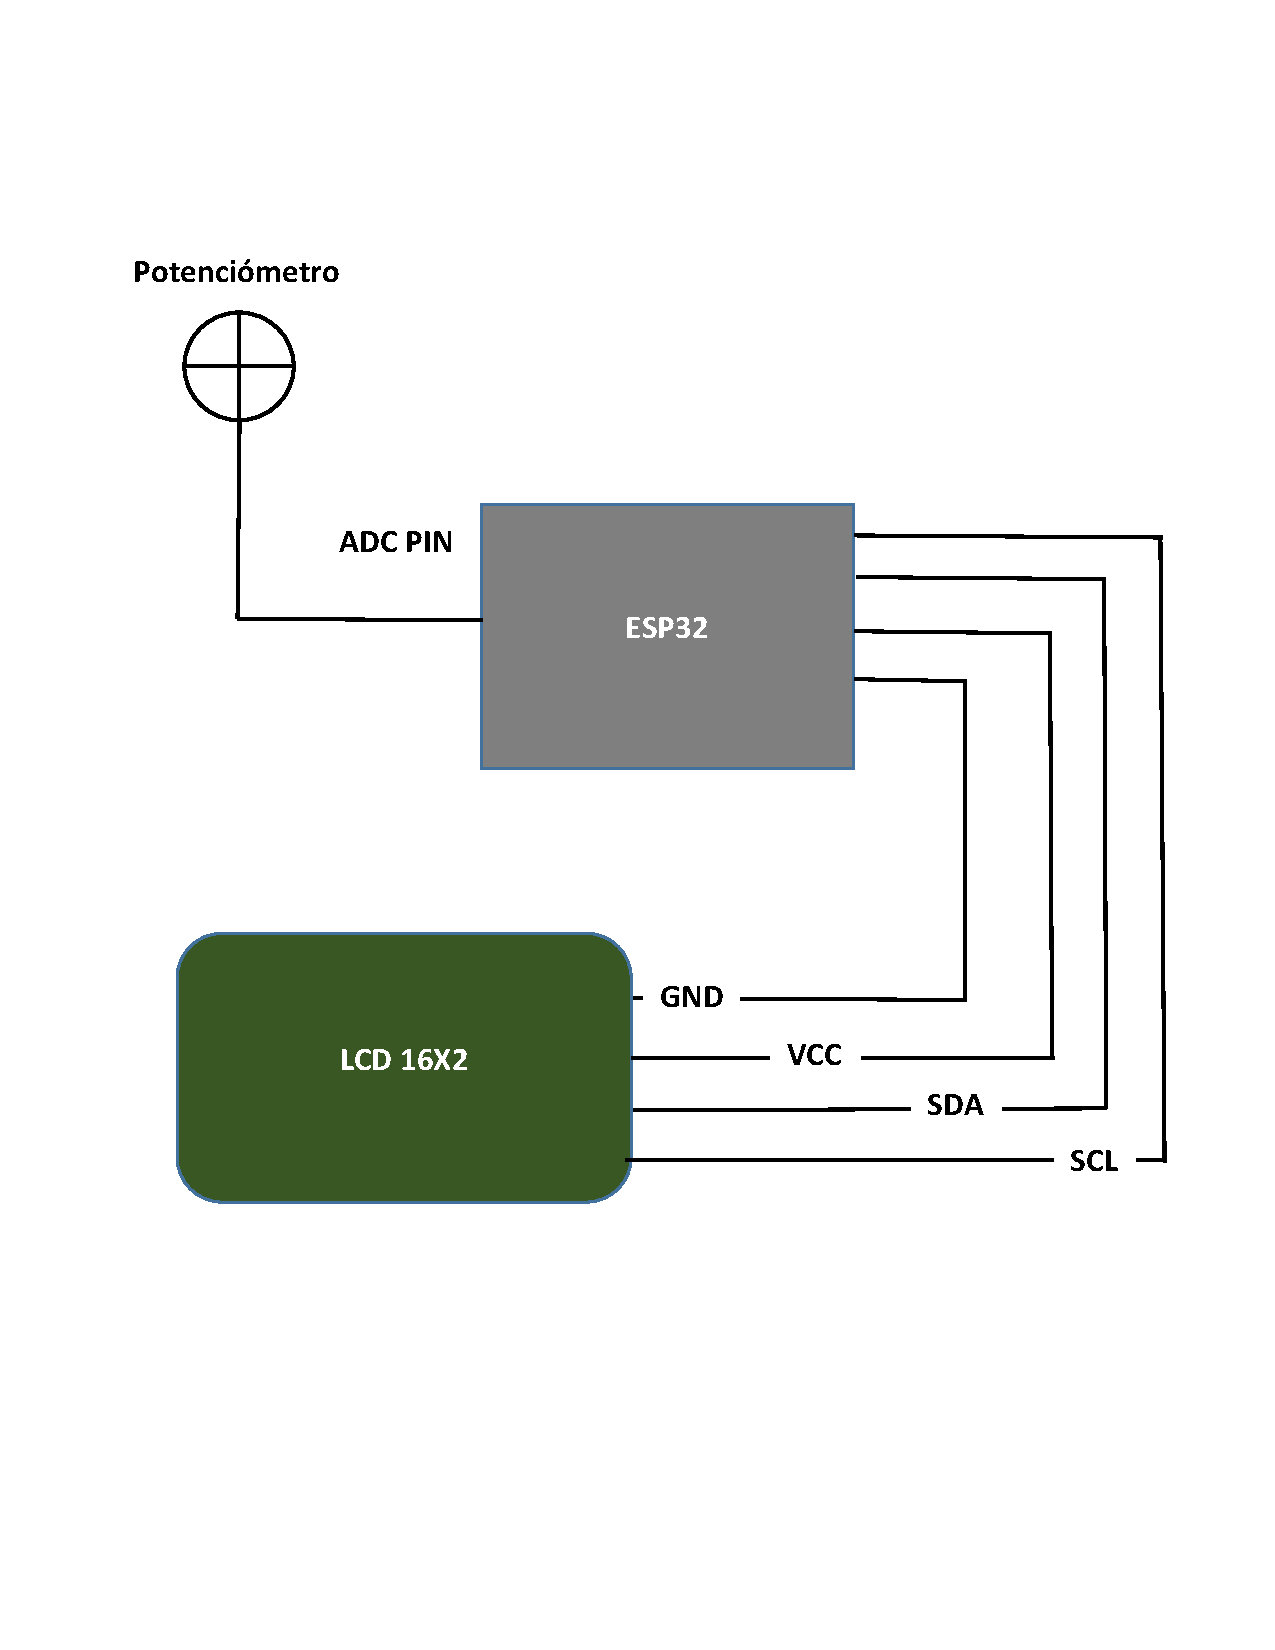
\includegraphics[trim = {15mm 15mm 15mm 15mm},clip,scale=0.35]{3/Img/cadenaDeMedida.pdf}
        \caption{Cadena de medida.}
        \label{fig:cadena de medida}
    \end{figure}
    % 
    % 
    \begin{figure}[H]
        \centering
        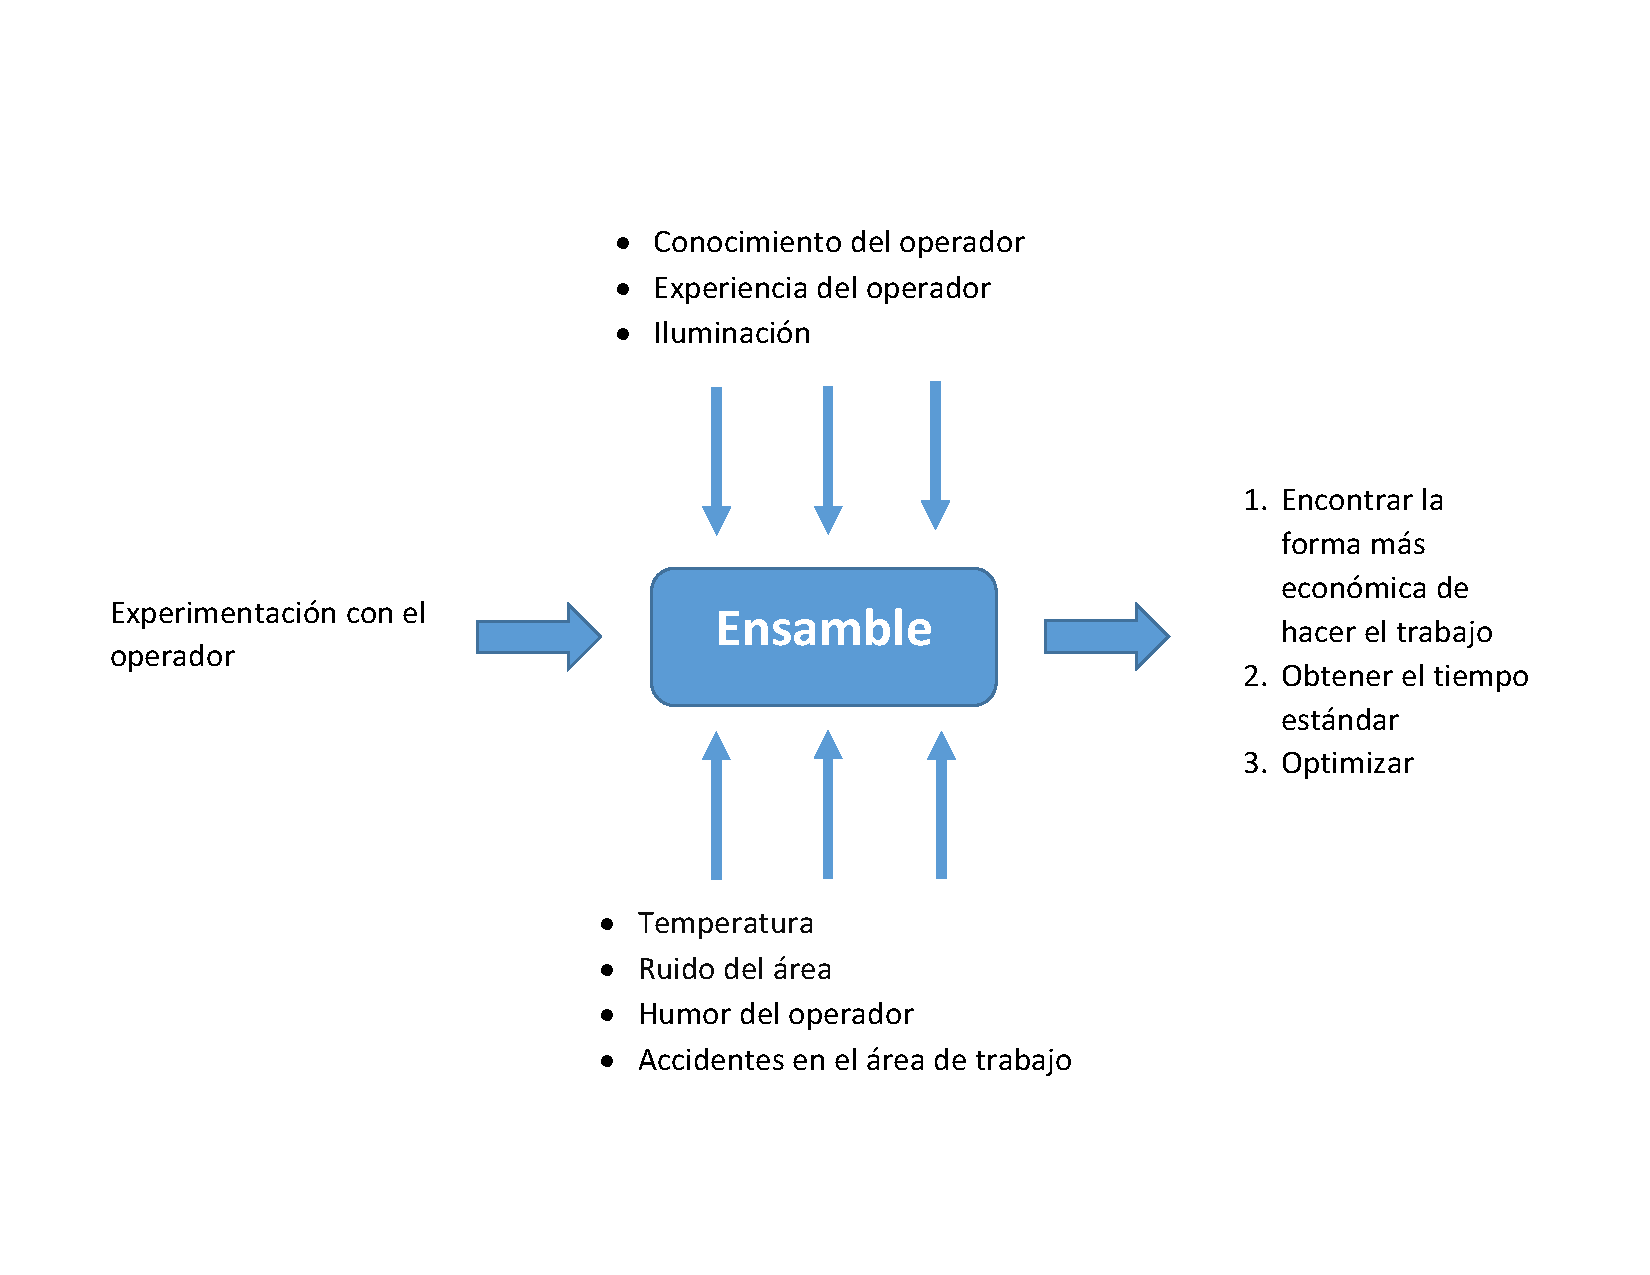
\includegraphics[trim = {15mm 0mm 0mm 0mm},clip,scale=0.35]{3/Img/diagramaDeEntradasySalidas.pdf}
        \caption{Diagrama de entradas y salidas para ilustrar la relación entre los componentes del sistema y cómo interactúan entre sí.}
        \label{fig:diagrama de entradas y salidas}
    \end{figure}
    % 
    % 
    \begin{itemize}
    \item Véase hoja de registro \ref{anexo:hojaDeRegistro}.
        \item Véase ensamble de circuito electrónico \ref{anexo:ensambleDeCircuitoElectrónico1}
    \end{itemize}
    % 
    % 
    \subsection{Desarrollo de la guía de plan de Emergencia}
    
    El Plan de Emergencia es un documento que detalla las directrices a seguir, la estructura organizativa y los procedimientos a implementar para manejar una situación de emergencia o desastre, abarcando tanto aspectos generales como específicos. Además, especifica cómo se deben utilizar de manera efectiva los recursos humanos y materiales disponibles.
    % 
    %
    \subsection{Análisis de los métodos, materiales, herramientas e instalación utilizada en la ejecución del ensamble de un circuito electrónico}
    
    \subsubsection{Planeación}
    % Asegúrate de conocer siempre tu objetivo.
    % Asegúrate de contar con los documentos (formatos, procedimientos, etc).
    Para este proyecto, nuestro objetivo es encontrar la manera más económica de realizar el trabajo. Nos centraremos en detectar áreas que pueden mejorarse, acortar el tiempo del ciclo de trabajo y eliminar movimientos innecesarios. Para ello, recopilaremos datos usando una cámara que grabará video continuamente, lo que nos permitirá medir el tiempo con precisión. Para llevar a cabo este ensamble de circuito electrónico, utilizaremos varios materiales que facilitarán el ensamblaje de manera óptima. El profesor nos ha dado una lista de los materiales necesarios. Véase los materiales en la figura \ref{fig:multicontactoFigura}.\ref{fig:cableUSB-CFigura}.\ref{fig:potenciómetroFigura}.\ref{fig:lcdFigura}.\ref{fig:móduloAdaptadorLcdFigura}.\ref{fig:esp32Figura}.\ref{fig:protoboardFigura}.\ref{fig:resistenciaFigura}.\ref{fig:cableMHFigura}.\ref{fig:cableMMFigura}.\ref{fig:tapeteProfesionalOrganizadorDeTrabajoFigura}
    % 
    % 
    \begin{figure}[H]
        \centering
        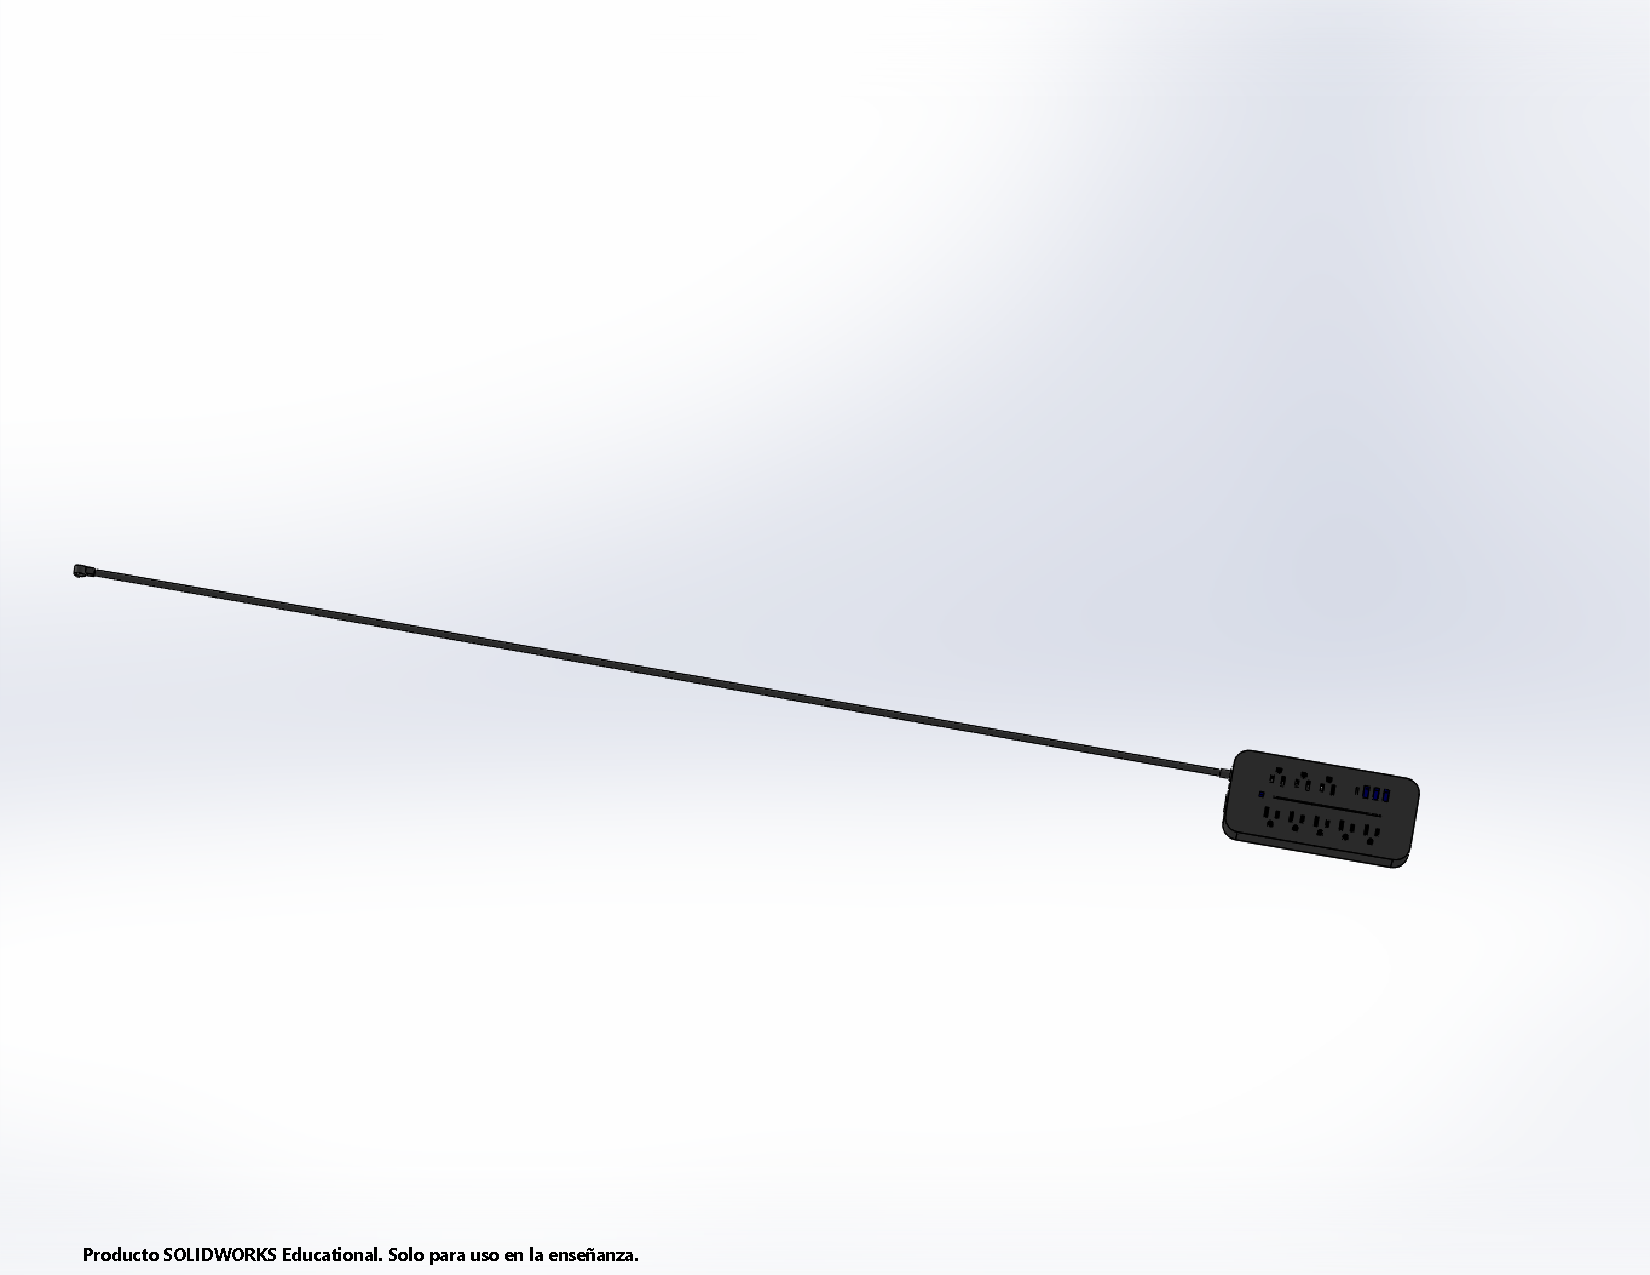
\includegraphics[trim = {5mm 50mm 15mm 60mm},clip,scale=0.2]{3/Img/multicontactoFigura.pdf}
        \caption{PC-01 Multicontacto}
        \label{fig:multicontactoFigura}
    \end{figure}
    % 
    % 
    \begin{figure}[H]
        \centering
        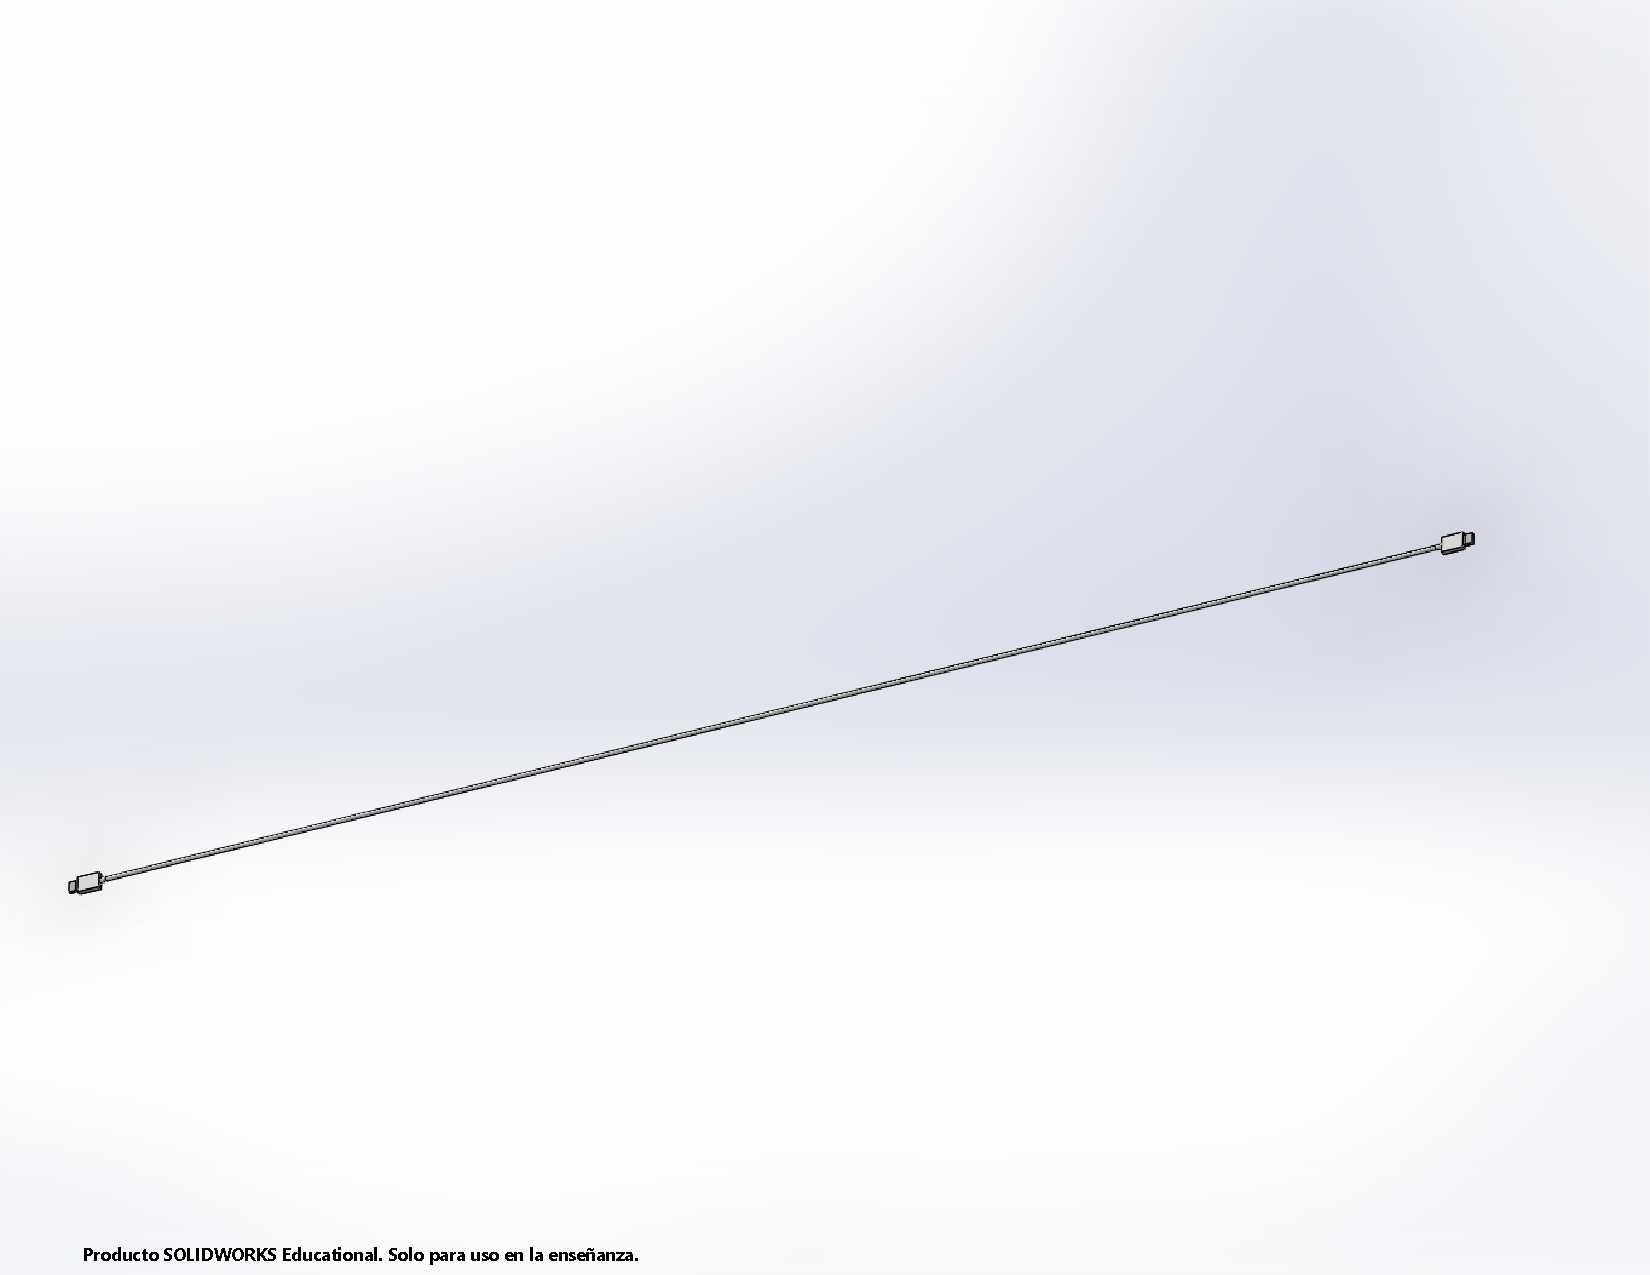
\includegraphics[trim = {1mm 50mm 1mm 60mm},clip,scale=0.2]{3/Img/cableUSB-CFigura.pdf}
        \caption{PC-02 Cable USB-C}
        \label{fig:cableUSB-CFigura}
    \end{figure}
    % 
    % 
    \begin{figure}[H]
        \centering
        \includegraphics[trim = {20mm 10mm 20mm 30mm},clip,scale=0.2]{3/Img/potenciómetroFigura.pdf}
        \caption{PC-03 Potenciómetro 3541H-1-102L 1k}
        \label{fig:potenciómetroFigura}
    \end{figure}
    % 
    % 
    \begin{figure}[H]
        \centering
        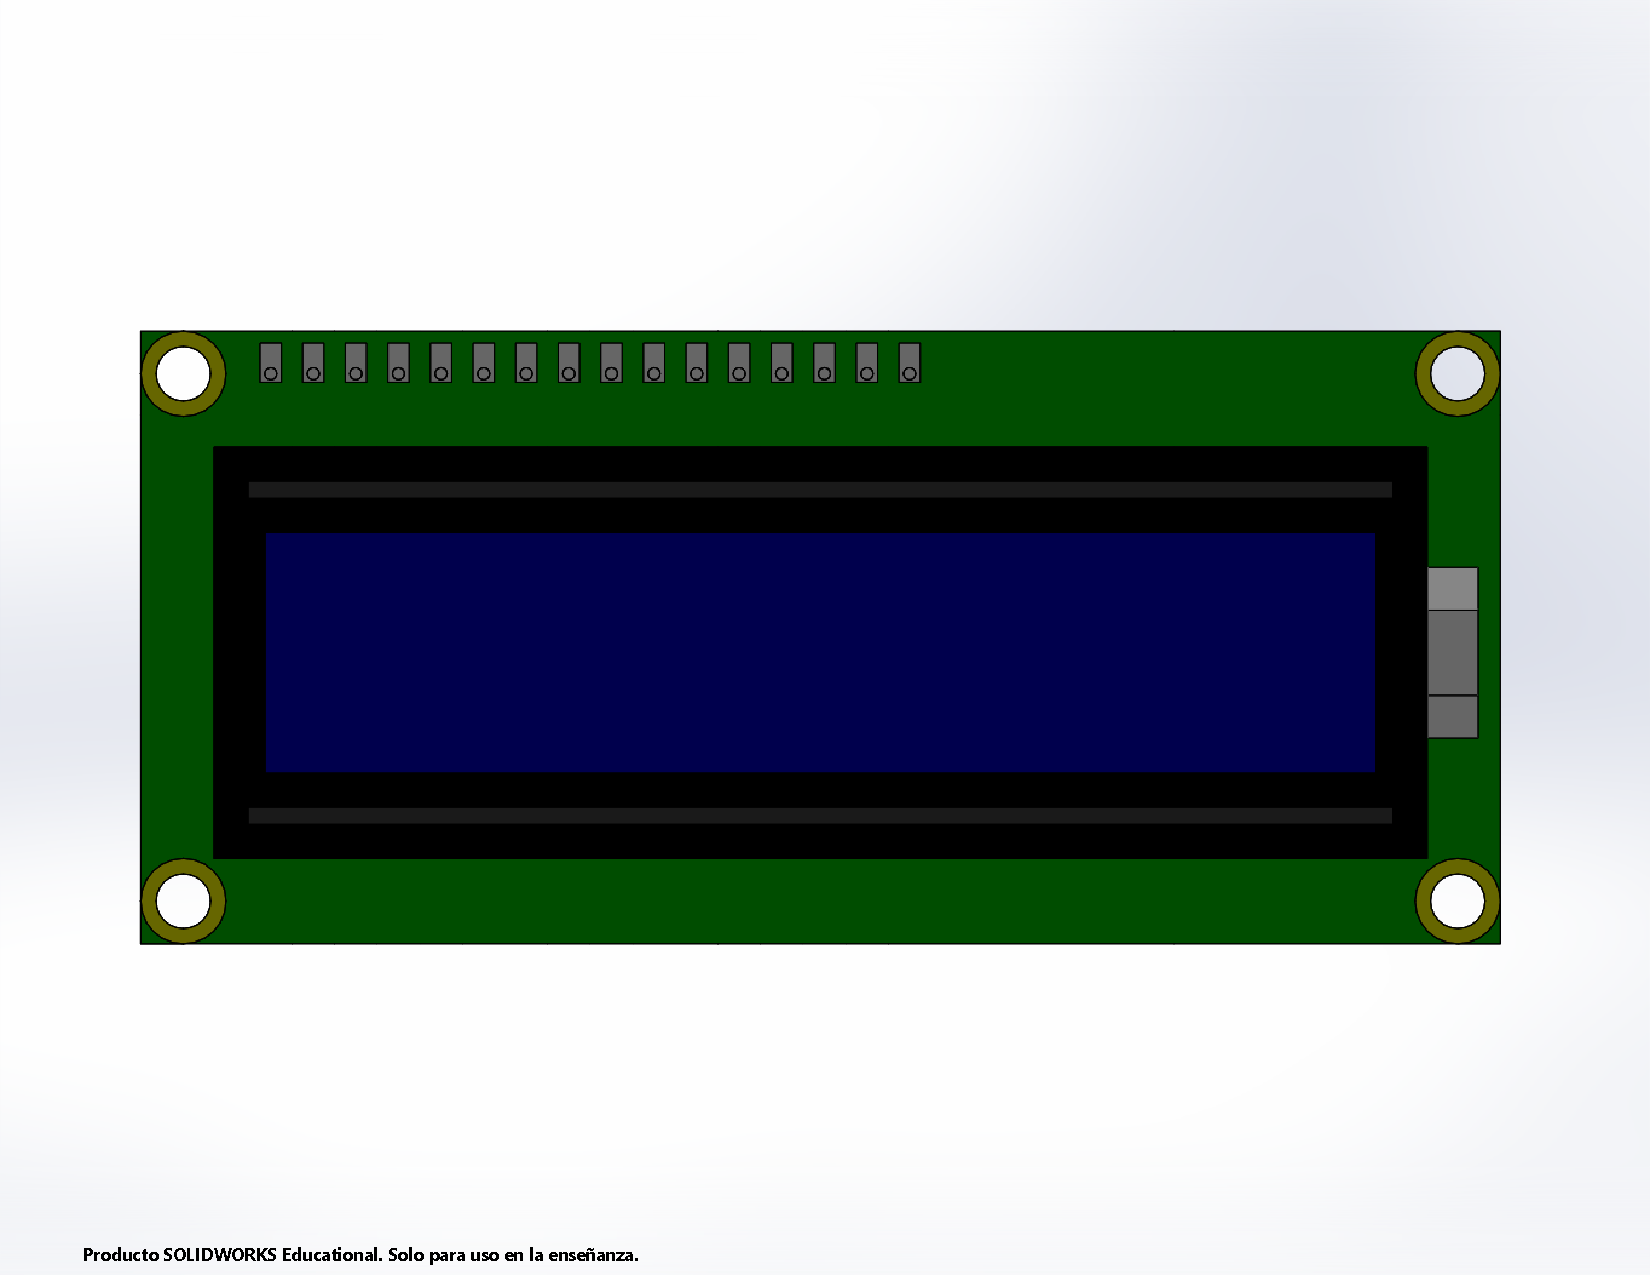
\includegraphics[trim = {1mm 20mm 1mm 20mm},clip,scale=0.2]{3/Img/lcdFigura.pdf}
        \caption{PC-04 LCD 16x2}
        \label{fig:lcdFigura}
    \end{figure}
    % 
    %
    \begin{figure}[H]
        \centering
        \includegraphics[trim = {1mm 10mm 1mm 1mm},clip,scale=0.2]{3/Img/móduloAdaptadorLcdFigura.PDF}
        \caption{PC-05 Módulo adaptador LCD 1602}
        \label{fig:móduloAdaptadorLcdFigura}
    \end{figure}
    % 
    %
    \begin{figure}[H]
        \centering
        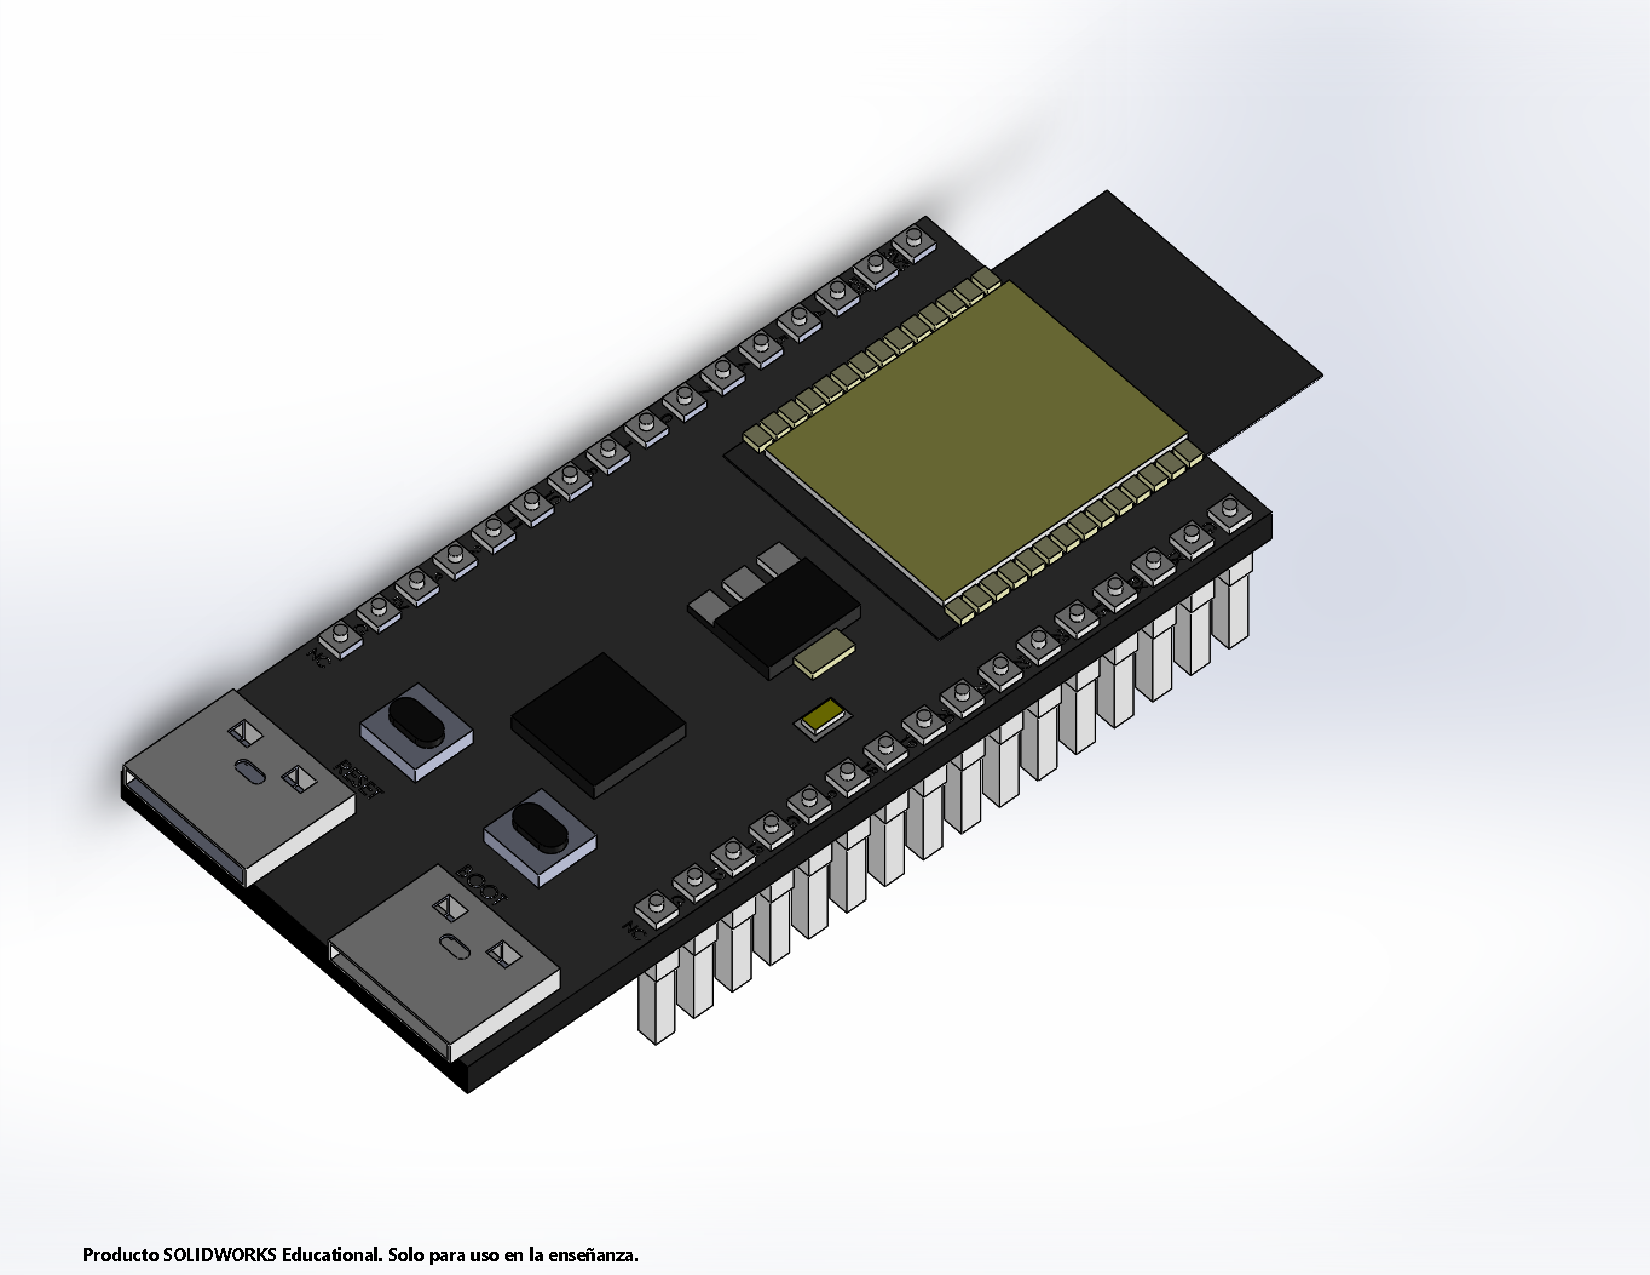
\includegraphics[trim = {1mm 10mm 20mm 1mm},clip,scale=0.2]{3/Img/esp32Figura.PDF}
        \caption{PC-06 ESP32-C6-WROOM-1}
        \label{fig:esp32Figura}
    \end{figure}
    % 
    %
    \begin{figure}[H]
        \centering
        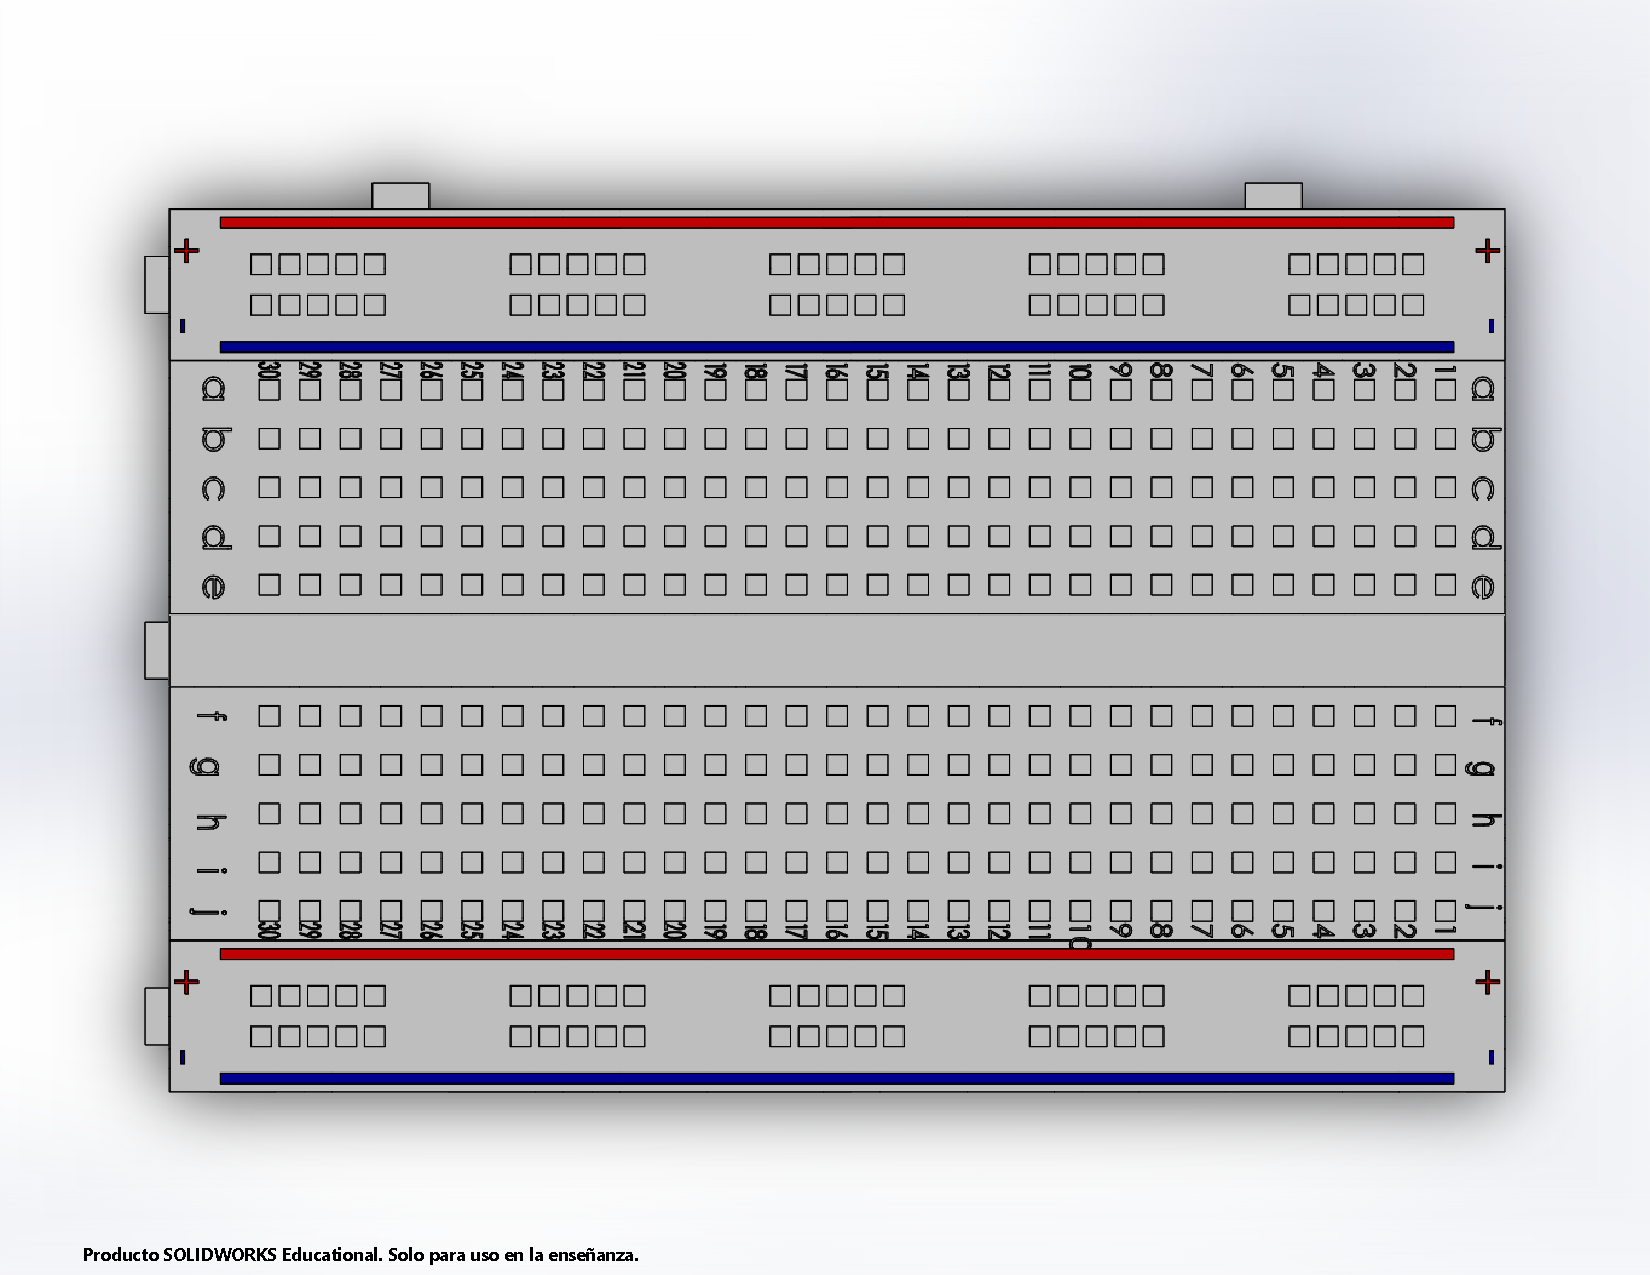
\includegraphics[trim = {1mm 10mm 1mm 1mm},clip,scale=0.2]{3/Img/protoboardFigura.PDF}
        \caption{PC-07 Protoboard}
        \label{fig:protoboardFigura}
    \end{figure}
    % 
    %
    \begin{figure}[H]
        \centering
        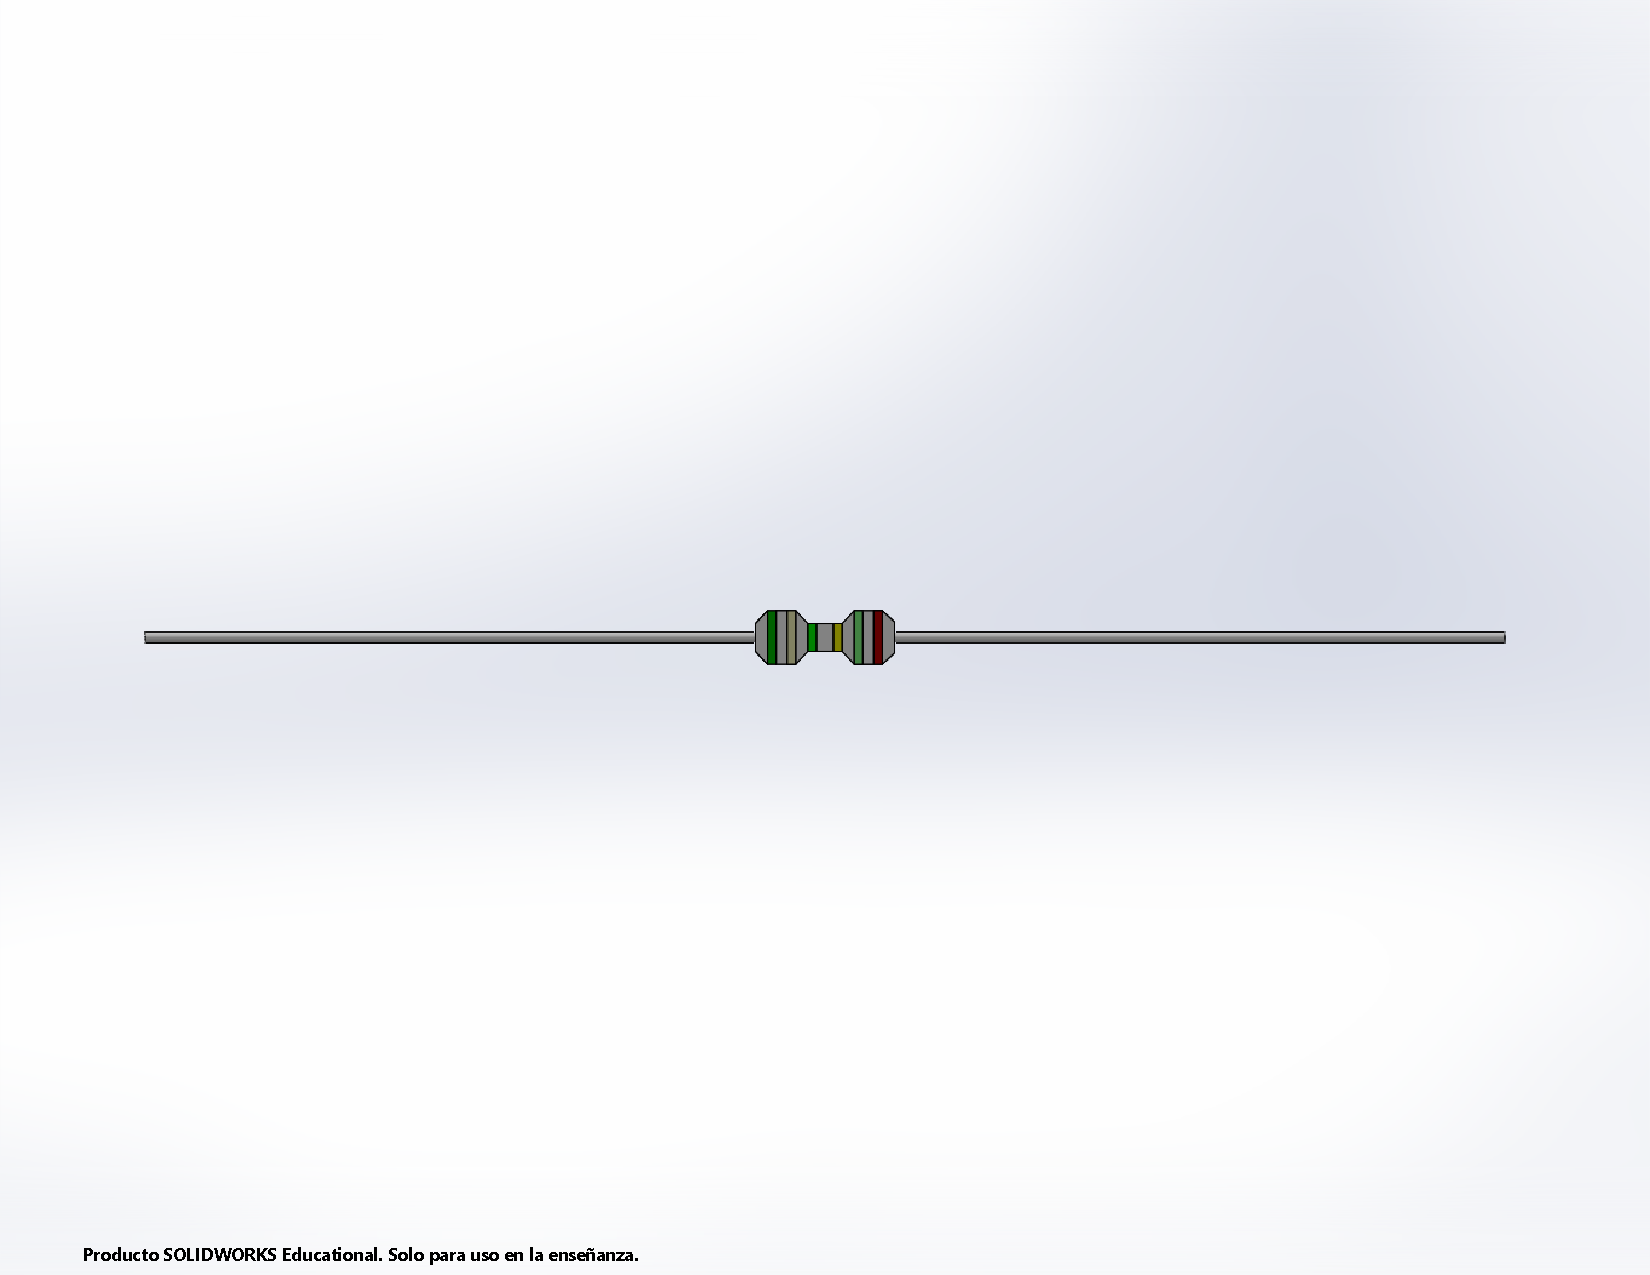
\includegraphics[trim = {1mm 50mm 1mm 50mm},clip,scale=0.2]{3/Img/resistenciaFigura.pdf}
        \caption{PC-08 Resistencia 330 1/4 W}
        \label{fig:resistenciaFigura}
    \end{figure}
    % 
    %
    \begin{figure}[H]
        \centering
        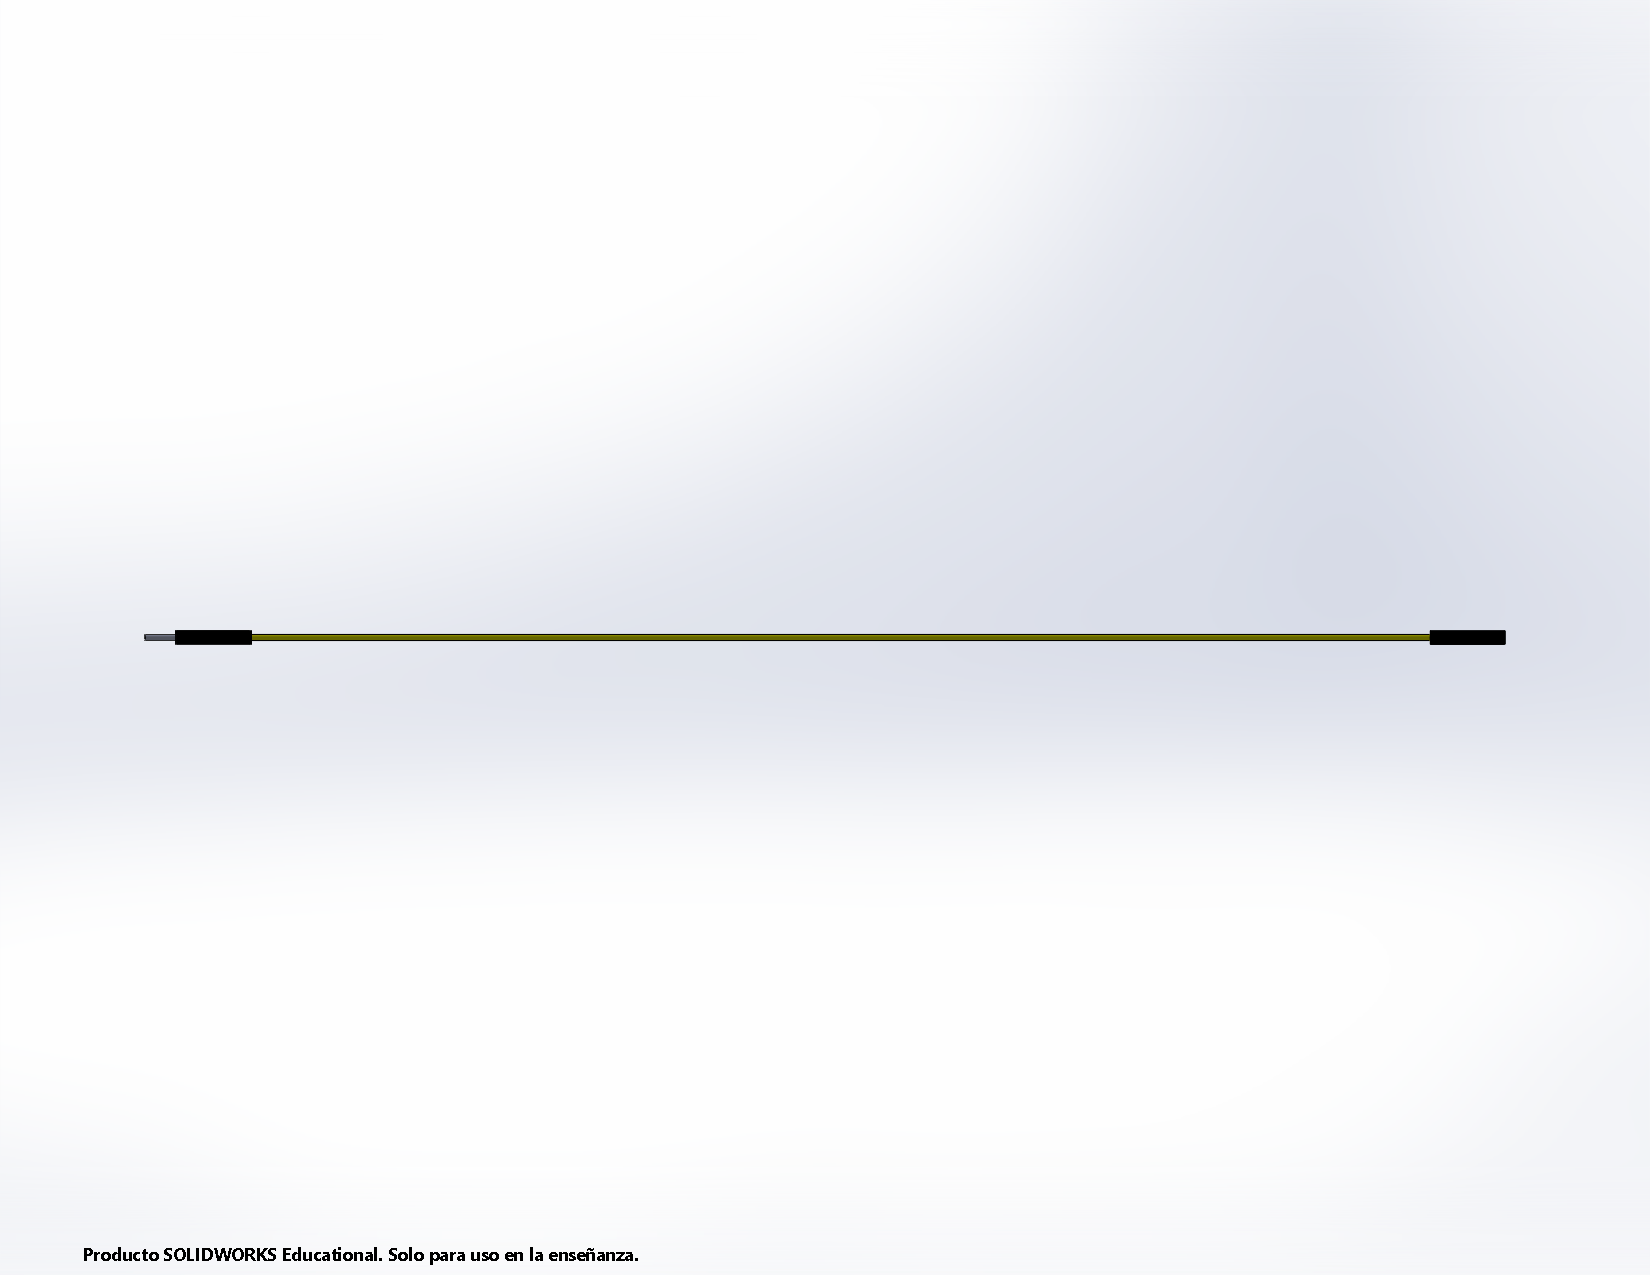
\includegraphics[trim = {1mm 50mm 1mm 50mm},clip,scale=0.2]{3/Img/cableMHFigura.pdf}
        \caption{PC-09 Cable MH 19cm}
        \label{fig:cableMHFigura}
    \end{figure}
    % 
    %
    \begin{figure}[H]
        \centering
        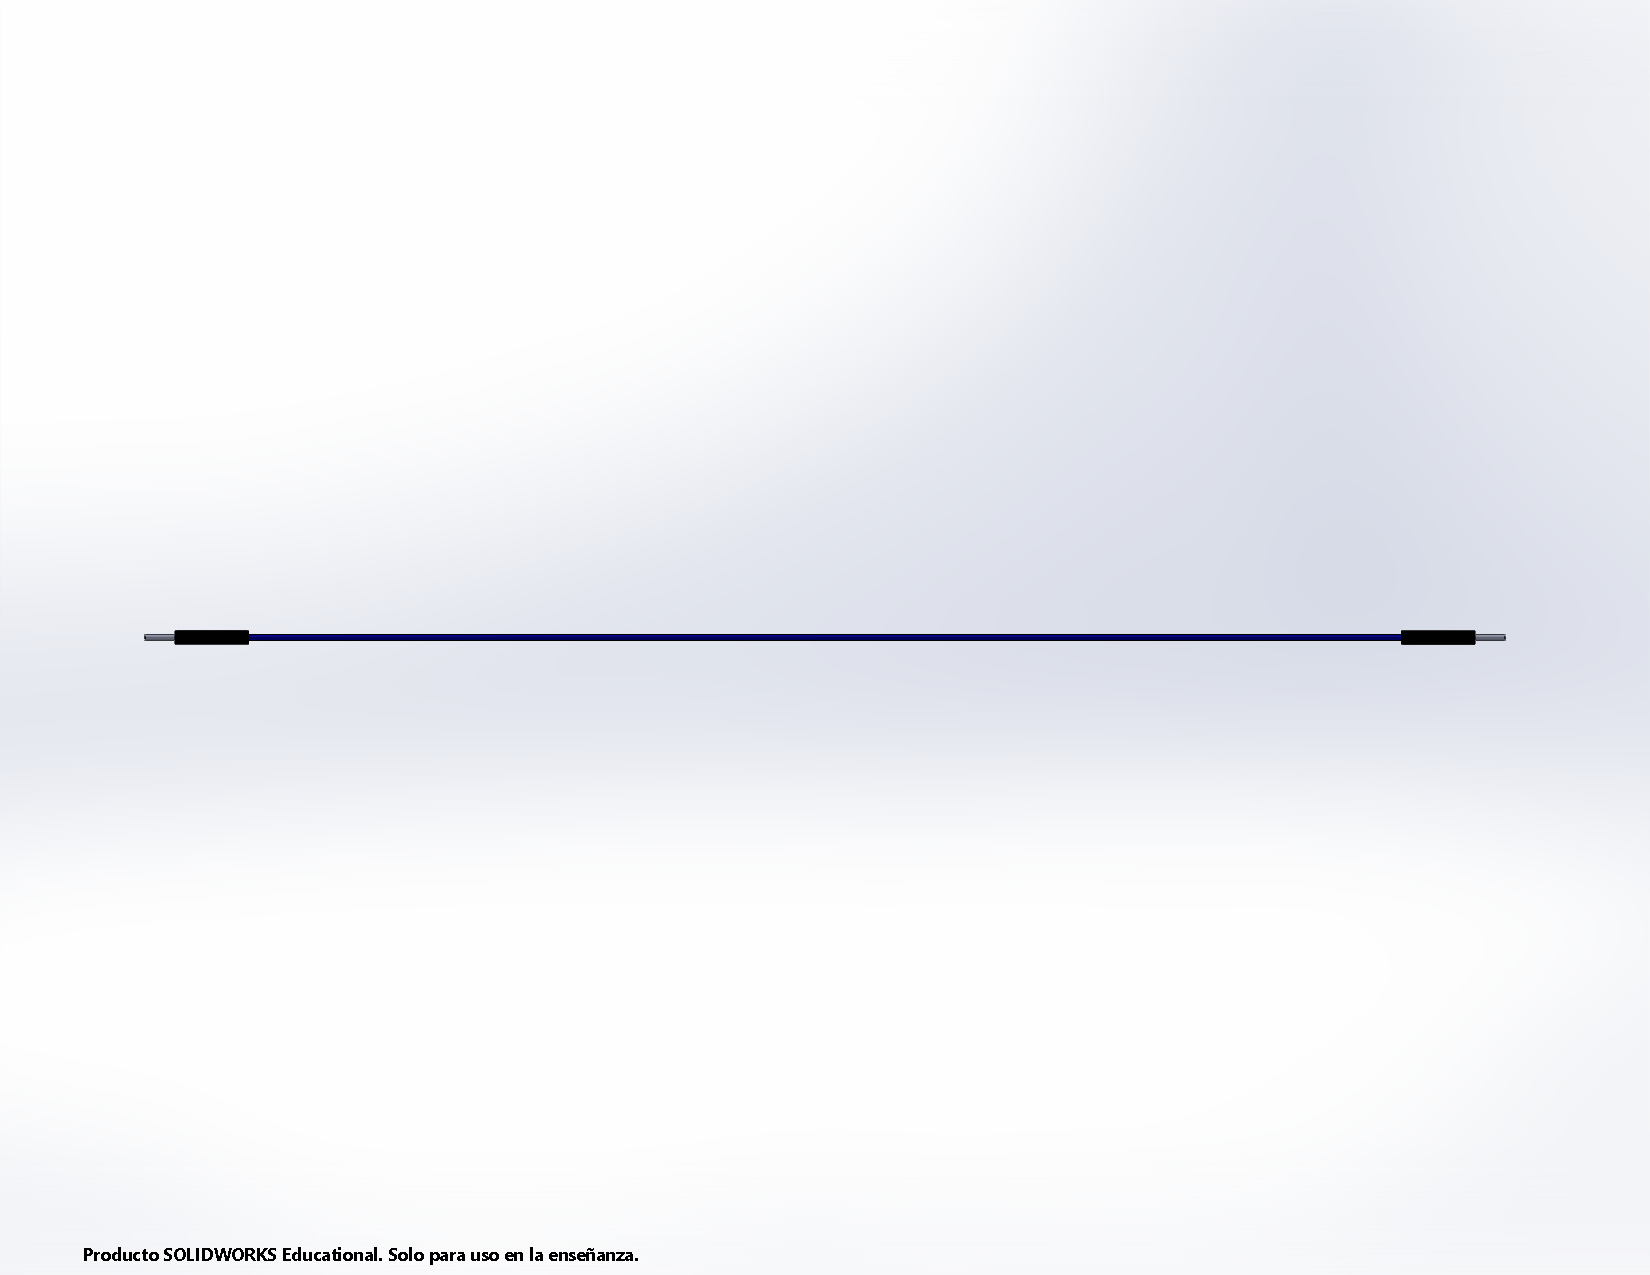
\includegraphics[trim = {1mm 50mm 1mm 50mm},clip,scale=0.2]{3/Img/cableMMFigura.pdf}
        \caption{PC-10 Cable MM 19cm}
        \label{fig:cableMMFigura}
    \end{figure}
    % 
    % 
    \begin{figure}[H]
        \centering
        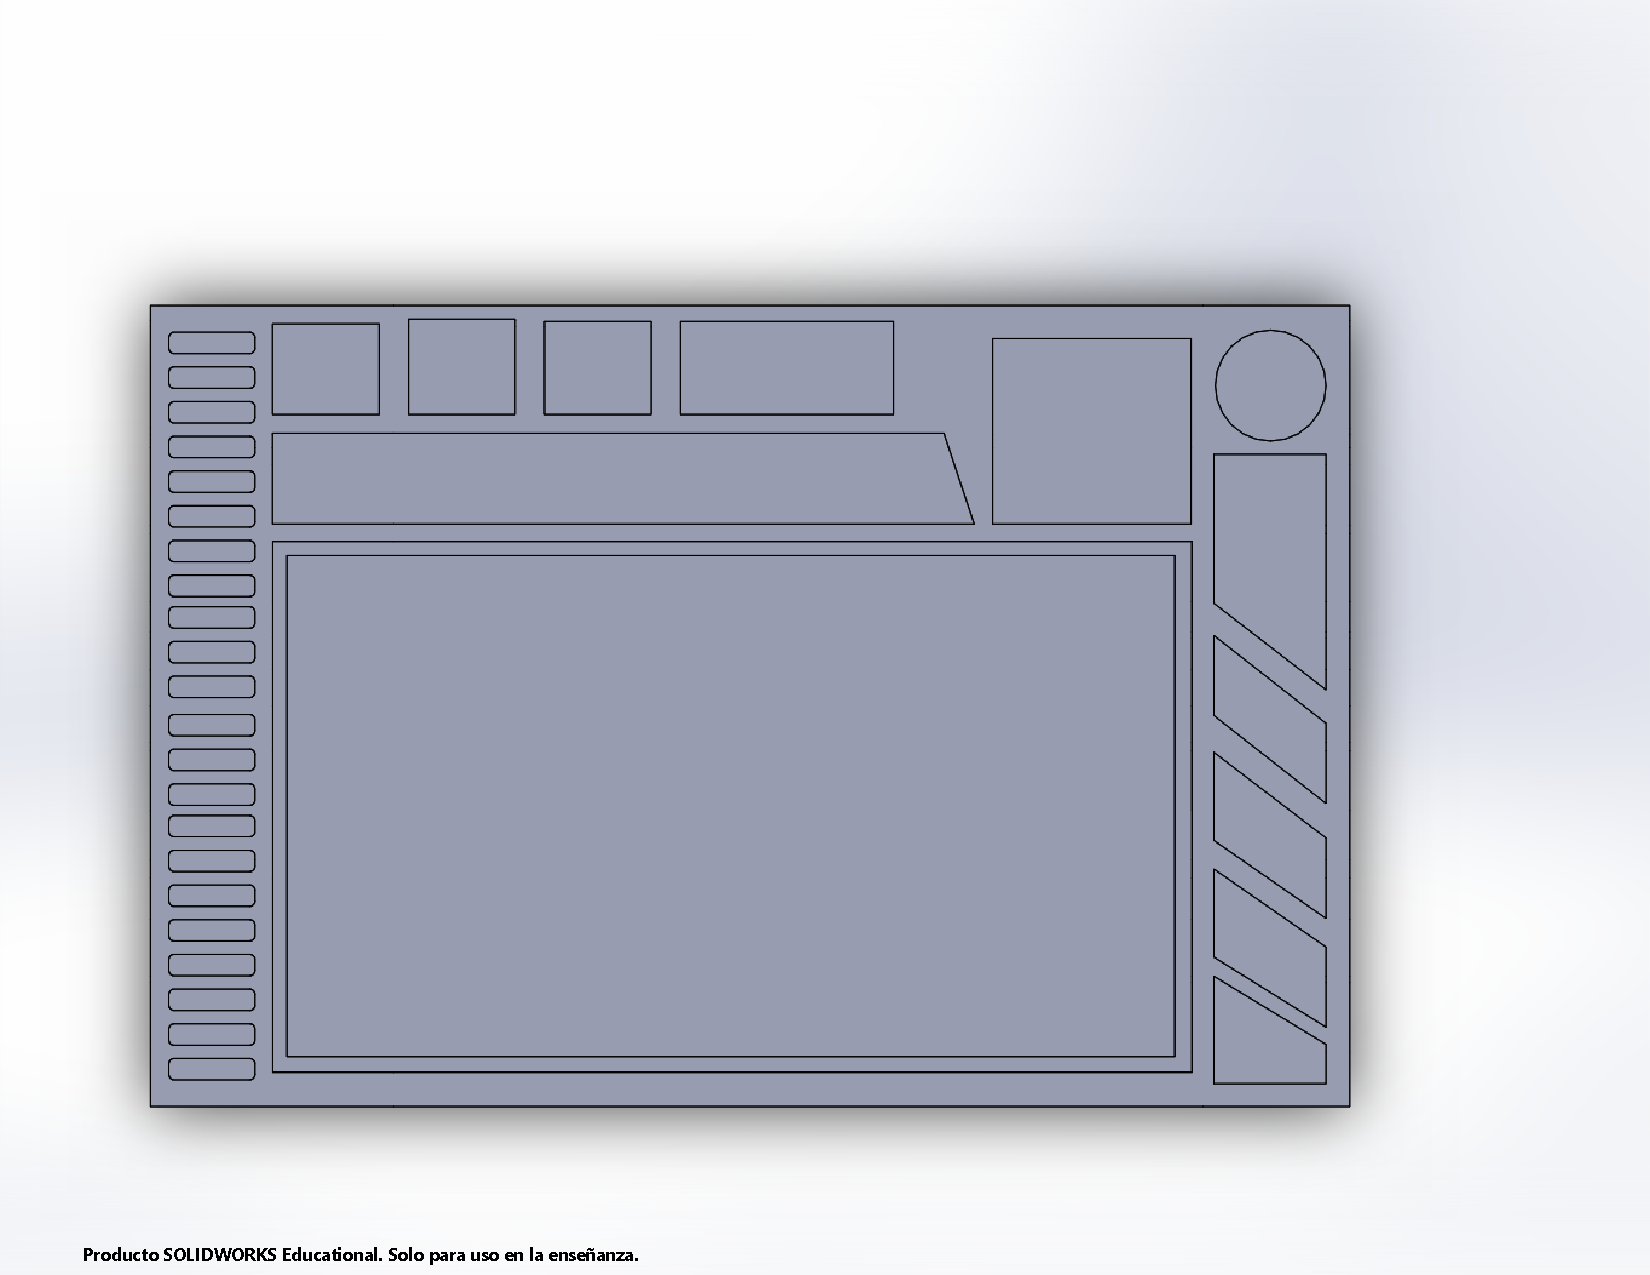
\includegraphics[trim = {1mm 10mm 30mm 30mm},clip,scale=0.2]{3/Img/tapeteProfesionalOrganizadorDeTrabajoFigura.pdf}
        \caption{PC-11 Tapete profesional organizador de trabajo}
        \label{fig:tapeteProfesionalOrganizadorDeTrabajoFigura}
    \end{figure}
    % 
    % 
    \subsubsection{5's}
    % ¿Qué son las 5’S?
    Consiste en tener un lugar de trabajo
    más ordenado, limpio y organizado que
    permite elevar la productividad y
    eficiencia en una empresa, haciéndolo de
    manera permanente.
    % ¿Para qué?
    Para generar eficiencia por medio de la
    reducción de desperdicios (ej. Esperas), tener un espacio limpio y ordenado, reflejar calidad en nuestro trabajo y evaluar los fundamentos de la cultura
    corporativa, en donde si no se pueden
    sustentar las 5´s, definitivamente no
    podremos aplicar ninguna herramienta de
    mejora.
    Las etapas son las siguientes: Seleccionar, Ordenar, Limpiar, Estandarizar, y Sostener.
    %
    % 
    Criterios para seleccionar
    \begin{itemize}
    \item Se deben de seleccionar las cosas
    que se necesitan y eliminar las
    innecesarias.
    \item Comúnmente se utilizan tarjetas
    donde indiquen la cantidad exacta.
    “Sólo lo que se necesita cuando se
    necesita”. 
    \end{itemize}
    % 
    % 
    Ordenar. Recomendaciones:
    \begin{itemize}
    \item Para objetos que sean de alto uso se
    recomienda que se tenga al alcance
    de la mano.
    \item Uso medio se debe colocar el objeto
    a escasos 7 pasos.
    \item Uso bajo puedes ubicar los objetos a
    más de 7 pasos.
    \end{itemize}
    % 
    % 
    Limpiar
    \begin{itemize}
    \item Se deben mantener las áreas de trabajo,
    herramientas y equipos lo más limpio
    posible
    "No es más eficiente quien más limpia
    sino quien menos ensucia”.
    \end{itemize}
    % 
    % 
    Estandarizar
    \begin{itemize}
    \item Se deben tener bien definidas las guías o
    procedimientos para mantener ordenado y
    limpio el área de trabajo.
    \end{itemize}
    % 
    % 
    Sostener 
    \begin{itemize}
    \item Incentivar a tener cultura para que esta
    implementación no quede únicamente en
    una acción , si no sea un hábito.
    \end{itemize} \cite{YellowBelt}
    % 
    % 
    \subsubsection{Desarrollo del sistema de tiempos predeterminado}
    
    Los sistemas de tiempo predeterminado (STP) son un conjunto de reglas o métodos para determinar con anticipación la secuencia de sucesos.
    Los STP están basados en los Therbligs
    \begin{itemize}
    \item Dividieron el trabajo en elementos.
    \item Asignaron valores de tiempo a cada elemento.
    \item Sumaron los tiempos de los elementos. 
    \end{itemize}
    Los STP tuvieron su origen en los Therbligs. A partir de los Therbligs se crearon sistemas que pueden ser o no más precisos, más fáciles de aplicar, más consistentes, más pertinentes para una industria específica. En teoría, los STP, cuando son aplicados por un analista "capacitado", pueden predecir "con precisión" el tiempo necesario para hacer un trabajo. Véase la tabla \ref{fig:tablaTherbligs}
    % 
    % 
    \begin{figure}[H]
        \centering
        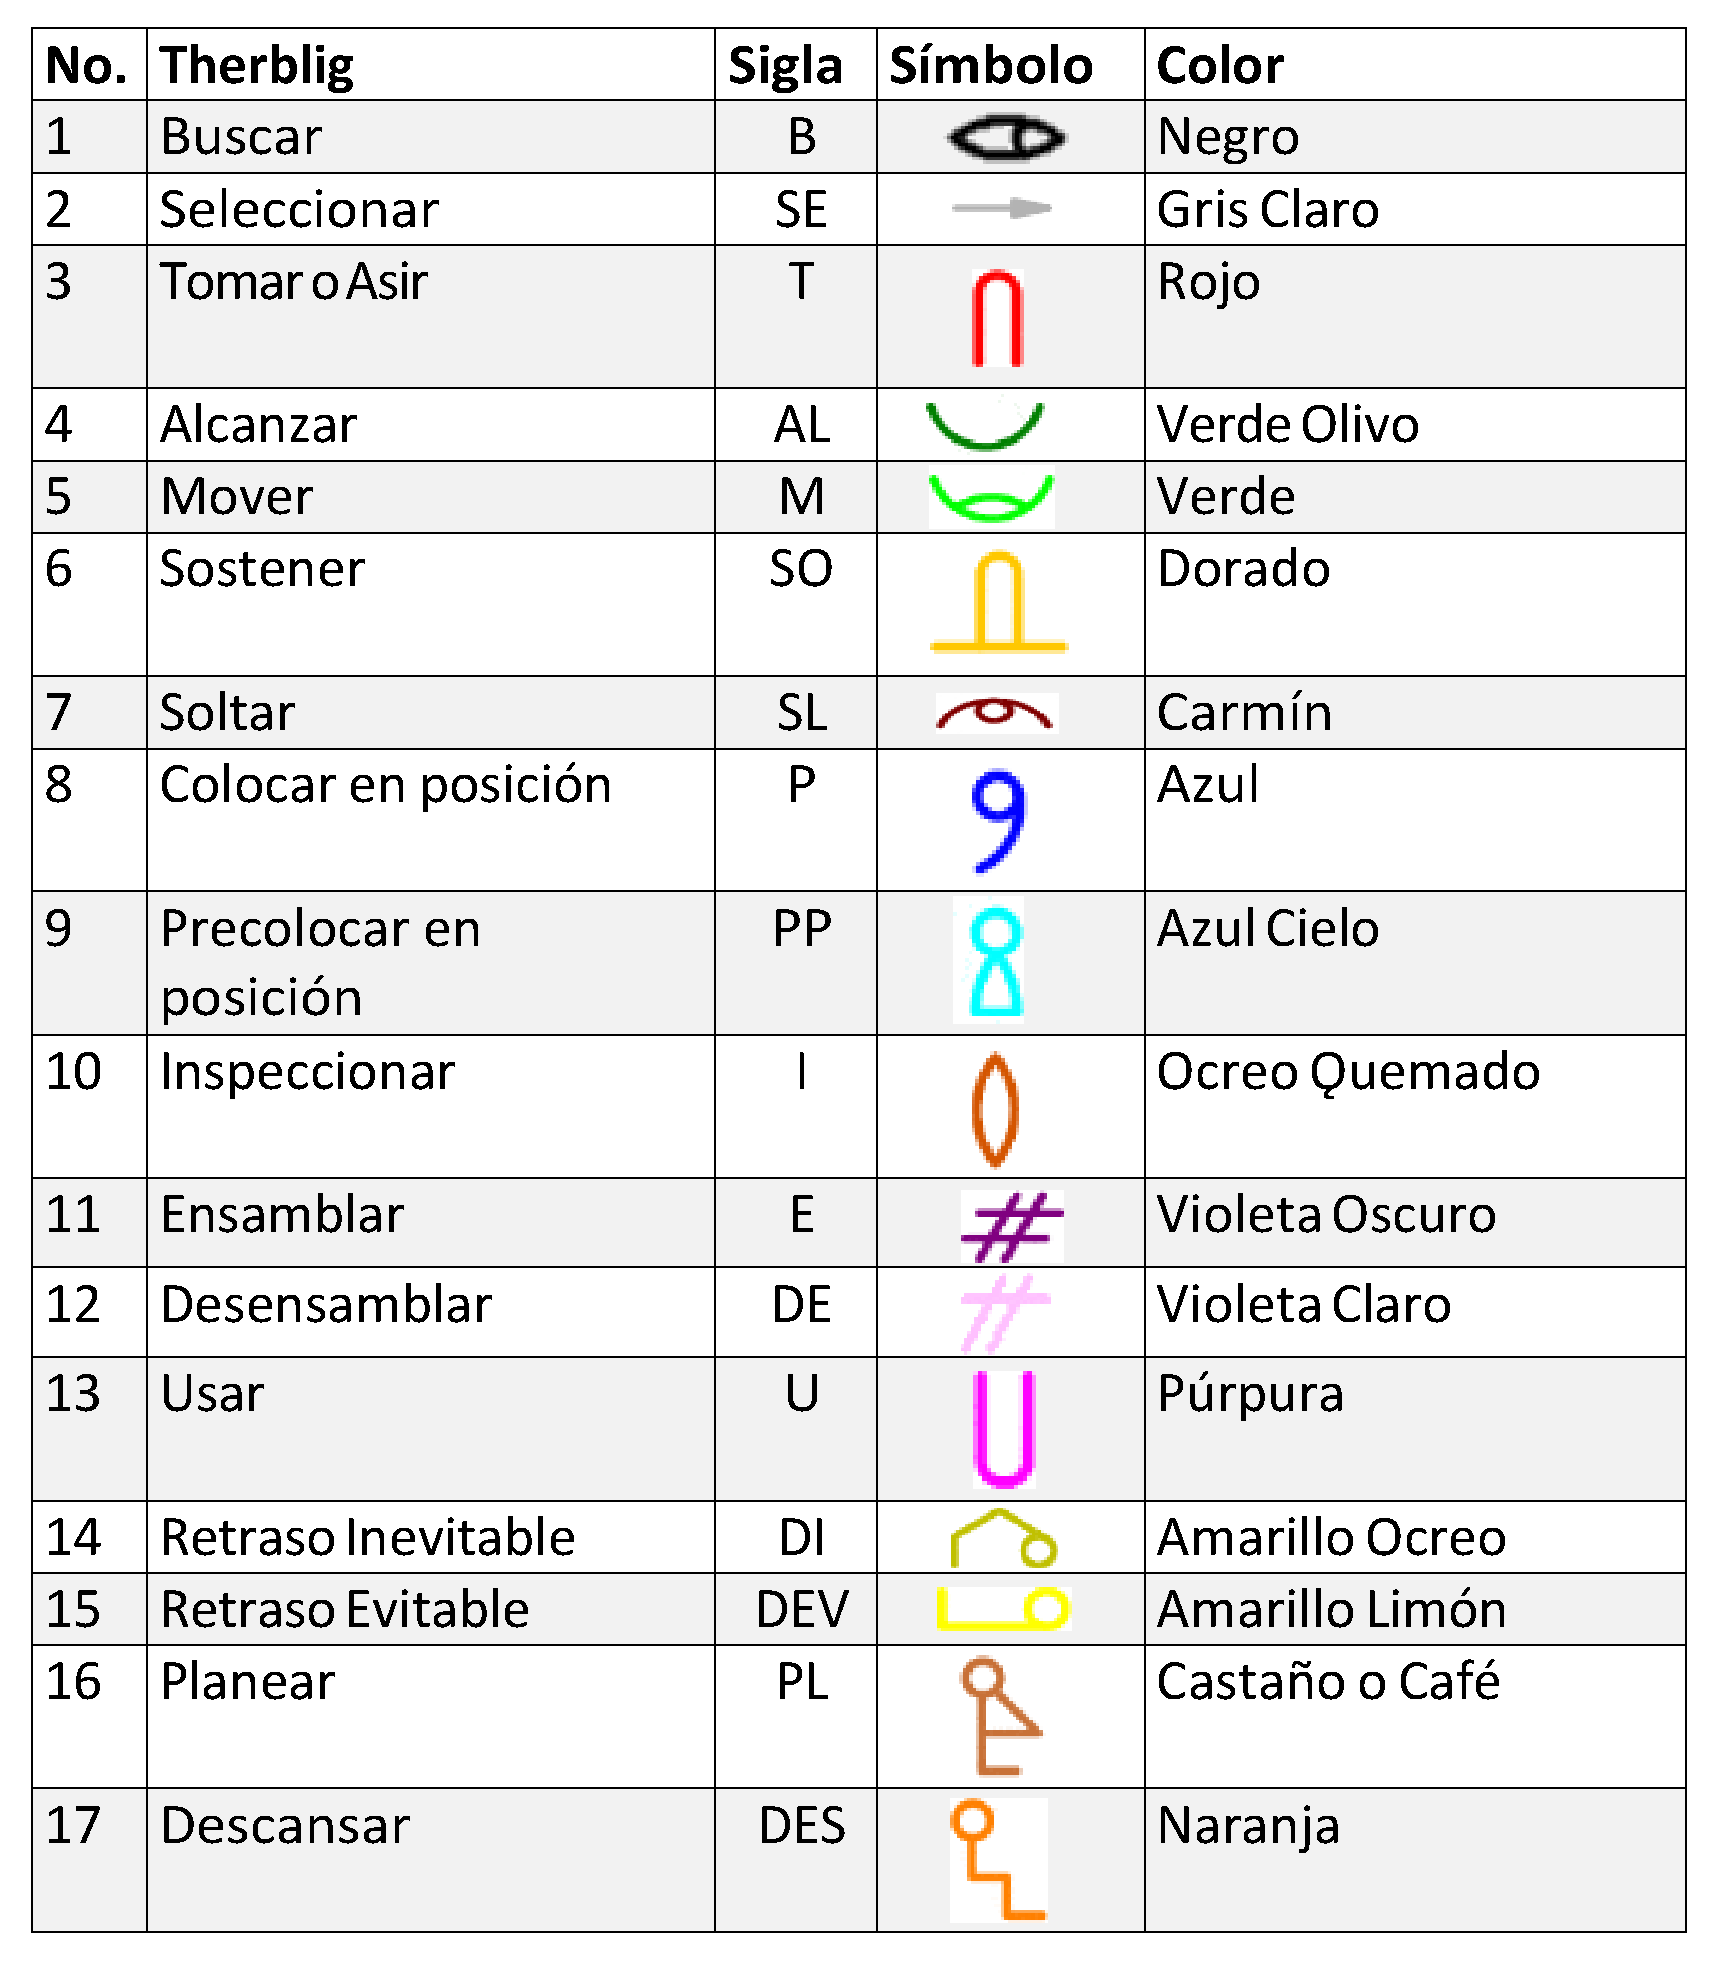
\includegraphics[scale=0.25]{3/Img/tablaTherblig.pdf}
        \caption{Tabla Therbligs.}
        \label{fig:tablaTherbligs}
    \end{figure}
    % 
    % 
    La finalidad de un estudio de STP es:
    \begin{itemize}
    \item Hacer un análisis de métodos para determinar un método eficiente de trabajo.
    \item Determinar el tiempo necesario para hacer el trabajo. 
    \end{itemize}
    La Medición de Tiempos de Métodos (MTM) es probablemente el STP que más se usa en el mundo. Existen diferentes MTM como el sistema básico (MTM-1) y dos sistemas simplificados (MTM-2 y MTM-3).
    El MTM-1 es un sistema que examina una operación y la divide en movimientos básicos necesarios para llevarla a cabo. Utiliza símbolos y abreviaturas predefinidos para identificarlos y asigna a cada movimiento básico un tiempo estándar predeterminado, basado en su naturaleza y en las condiciones en las que se realiza (TMU). Véase la tabla \ref{fig:tablaTMU}
    % 
    % 
    \begin{figure}[H]
        \centering
        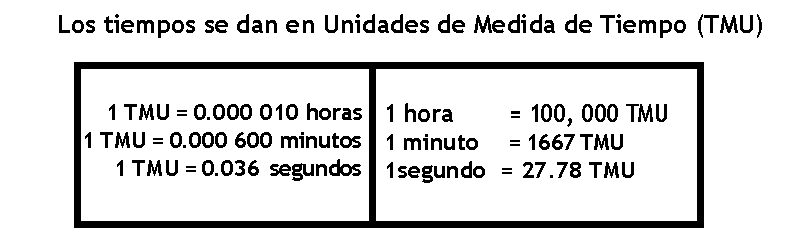
\includegraphics[scale=0.6]{3/Img/tablaTMU.pdf}
        \caption{Unidades de Medida De Tiempo (TMU).}
        \label{fig:tablaTMU}
    \end{figure}
    % 
    % 
    Estas son las tablas que utilizaré para para establecer métodos que aporten un alto nivel de productividad y tiempos muy precisos.
    
    Movimientos MTM-1:
    \begin{enumerate}
        \item Alcanzar: Se entiende como el movimiento realizado con la mano vacía, véase en la Figura \ref{fig:tabla1Alcanzar-R }
        \item Mover: Llevar un objeto a un lugar, véase en la Figura \ref{fig:tabla2Mover-M}
        \item Girar y Aplicar presión: Girar la mano respecto al eje largo del antebrazo, ensamblar, véase el caso A en la Figura \ref{fig:tabla3GirarYAplicarPresion-A} y caso B en la Figura \ref{fig:tabla3GirarYAplicarPresión-B}
        \item Asir: Control de uno o más objetos con los dedos o manos, véase en la Figura \ref{fig:tabla4Asir-G}
        \item Colocar en posición: Alinear, orientar o engranar un objeto con otro, véase en la Figura \ref{fig:tabla5ColocarEnPosición-P}
        \item Soltar: Entregar el control de un objeto, véase en la Figura \ref{fig:tabla6Soltar-RL}
        \item Desenganchar: Romper el contacto con el objeto, separar, desensamblar, véase en la Figura \ref{fig:tabla7Desenganche-D}
        \item Tiempo de desplazamiento de ojo y enfoque ocular: Los ojos dirigen movimientos de las manos o el cuerpo, véase en la Figura \ref{fig:tabla8TiempoDeDesplazamientoDeOjo}
        \item Movimientos de cuerpo, pierna y pie: Los movimientos se realizan con todo el cuerpo, véase en la Figura \ref{fig:tabla9MovimientosDeCuerpoPiernaYPie} 
        \item Movimientos Simultáneos: Dificultad con la que se realizan los movimientos antes mencionados, véase en la Figura \ref{fig:tabla10MovimientosSimultaneos}
    \end{enumerate}
    % 
    % 
    \begin{figure}[H]
        \centering
        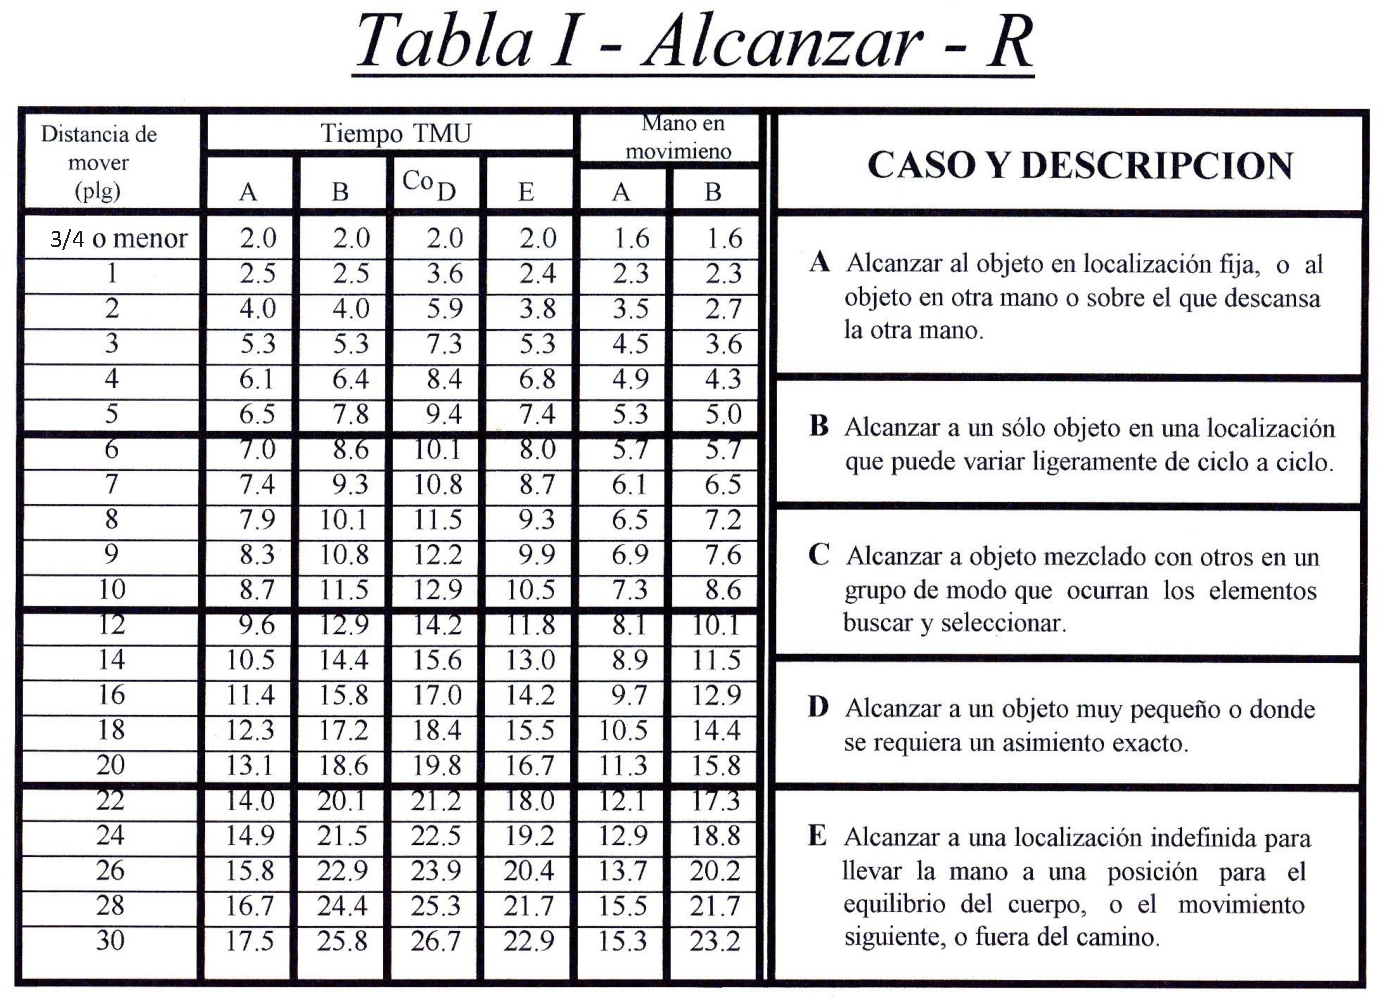
\includegraphics[scale=0.32]{3/Img/tabla1Alcanzar-R .pdf}
        \caption{Valores estándar del Therblig Alcanzar-R.}
        \label{fig:tabla1Alcanzar-R }
    \end{figure}
    % 
    % 
    \begin{figure}[H]
        \centering
        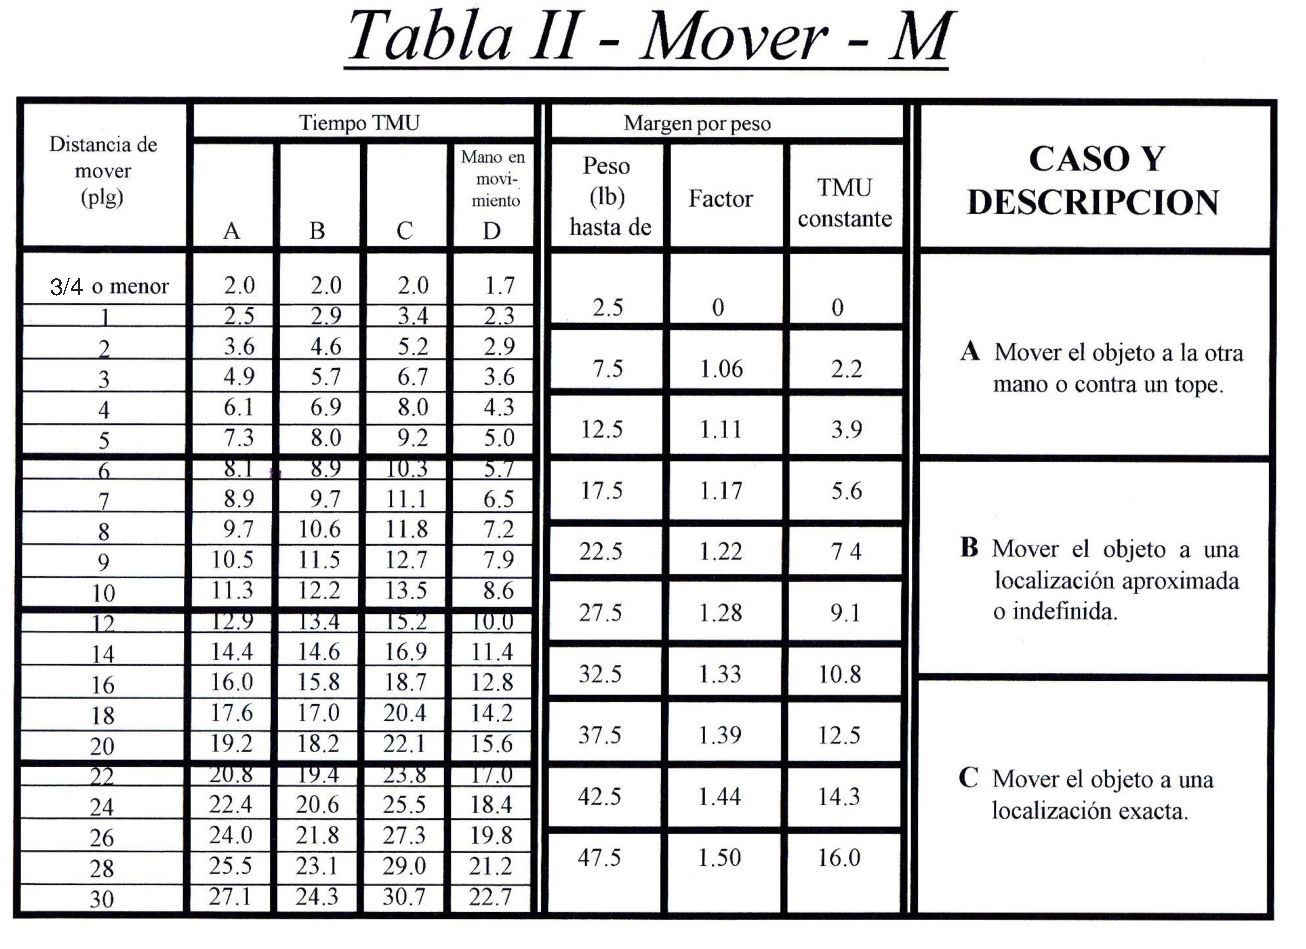
\includegraphics[scale=0.35]{3/Img/tabla2Mover-M.pdf}
        \caption{Valores estándar del Therblig Mover-M.}
        \label{fig:tabla2Mover-M}
    \end{figure}
    % 
    % 
    \begin{figure}[H]
        \centering
        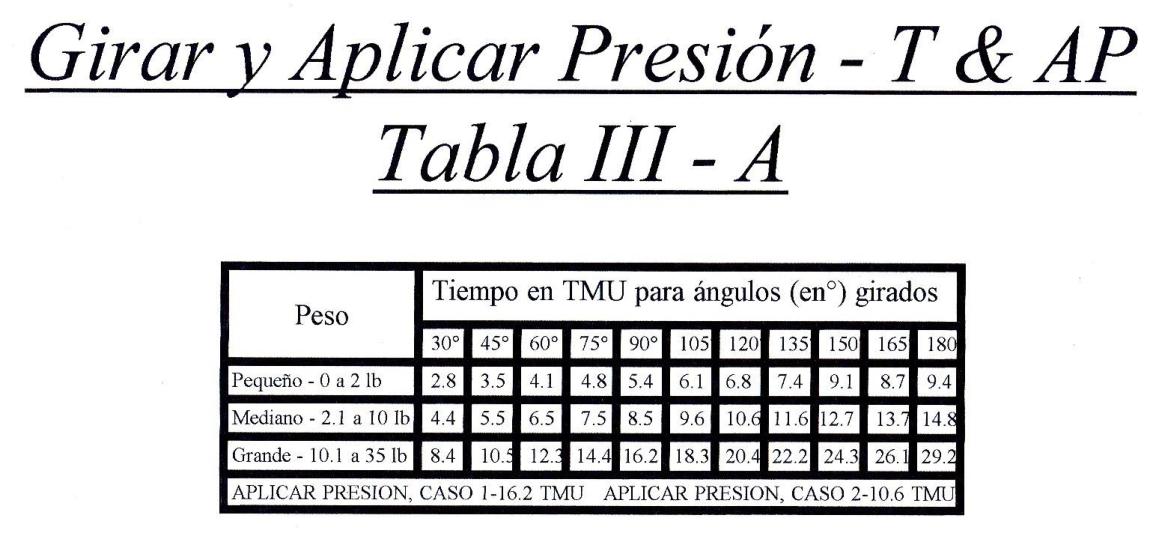
\includegraphics[scale=0.4]{3/Img/tabla3GirarYAplicarPresion-A.pdf}
        \caption{Valores estándar del Therblig Girar y Aplicar Presión-A.}
        \label{fig:tabla3GirarYAplicarPresion-A}
    \end{figure}
    % 
    % 
    \begin{figure}[H]
        \centering
        \includegraphics[scale=0.4]{3/Img/tabla3GirarYAplicarPresión-B.pdf}
        \caption{Valores estándar del Therblig Girar y Aplicar Presión-B.}
        \label{fig:tabla3GirarYAplicarPresión-B}
    \end{figure}
    % 
    % 
    \begin{figure}[H]
        \centering
        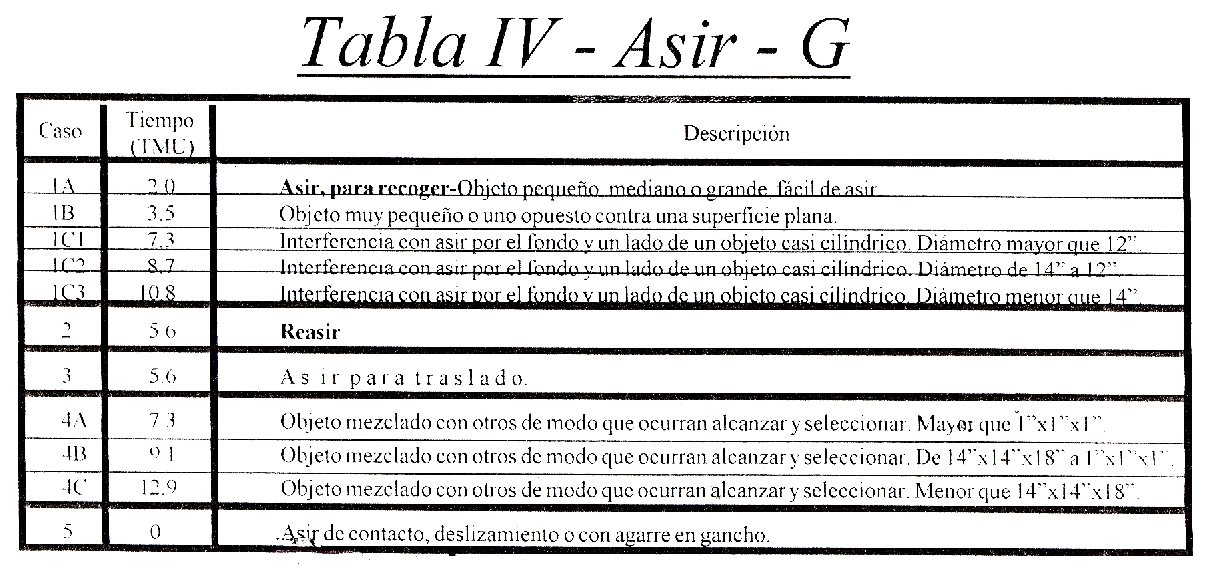
\includegraphics[scale=0.4]{3/Img/tabla4Asir-G.pdf}
        \caption{Valores estándar del Therblig Asir-G.}
        \label{fig:tabla4Asir-G}
    \end{figure}
    % 
    %
    \begin{figure}[H]
        \centering
        \includegraphics[scale=0.45]{3/Img/tabla5ColocarEnPosición-P.pdf}
        \caption{Valores estándar del Therblig Colocar en Posición-P.}
        \label{fig:tabla5ColocarEnPosición-P}
    \end{figure}
    % 
    % 
    \begin{figure}[H]    
        \centering
        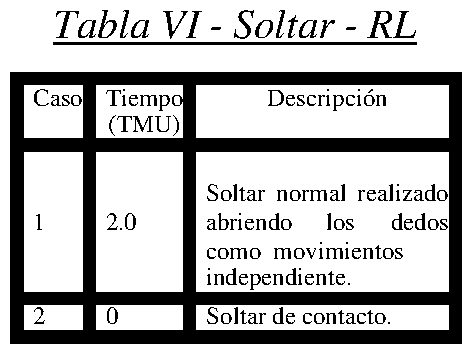
\includegraphics[scale=0.6]{3/Img/tabla6Soltar-RL.pdf}
        \caption{Valores estándar del Therblig Soltar-RL.}
        \label{fig:tabla6Soltar-RL}
    \end{figure}
    % 
    % 
    \begin{figure}[H]
        \centering
        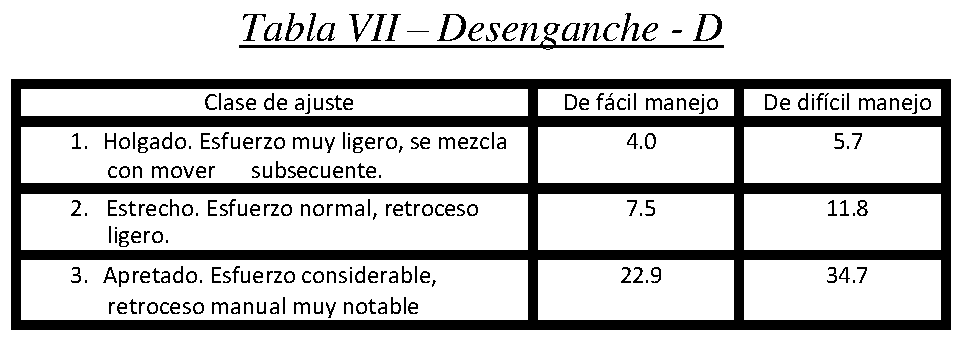
\includegraphics[scale=0.5]{3/Img/tabla7Desenganche-D.pdf}
        \caption{Valores estándar del Therblig Desenganche-D.}
        \label{fig:tabla7Desenganche-D}
    \end{figure}
    % 
    %
    \begin{figure}[H]
        \centering
        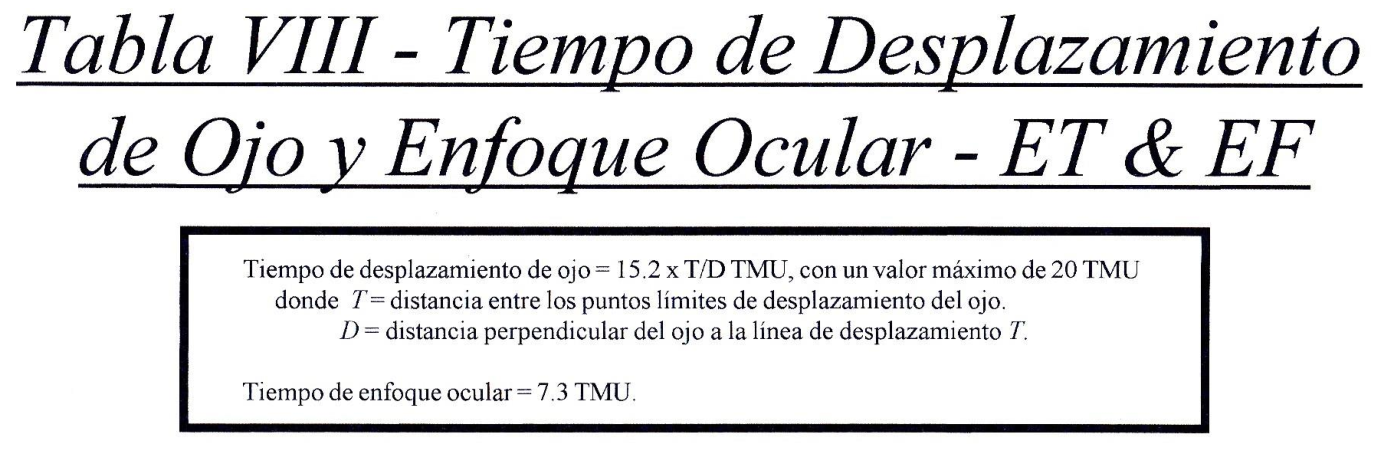
\includegraphics[scale=0.35]{3/Img/tabla8TiempoDeDesplazamientoDeOjo.pdf}
        \caption{Valores estándar del Therblig Tiempo de Desplazamiento de Ojo y Enfoque Ocular-ET y EF.}
        \label{fig:tabla8TiempoDeDesplazamientoDeOjo}
    \end{figure}
    % 
    % 
    \begin{figure}[H]
        \centering
        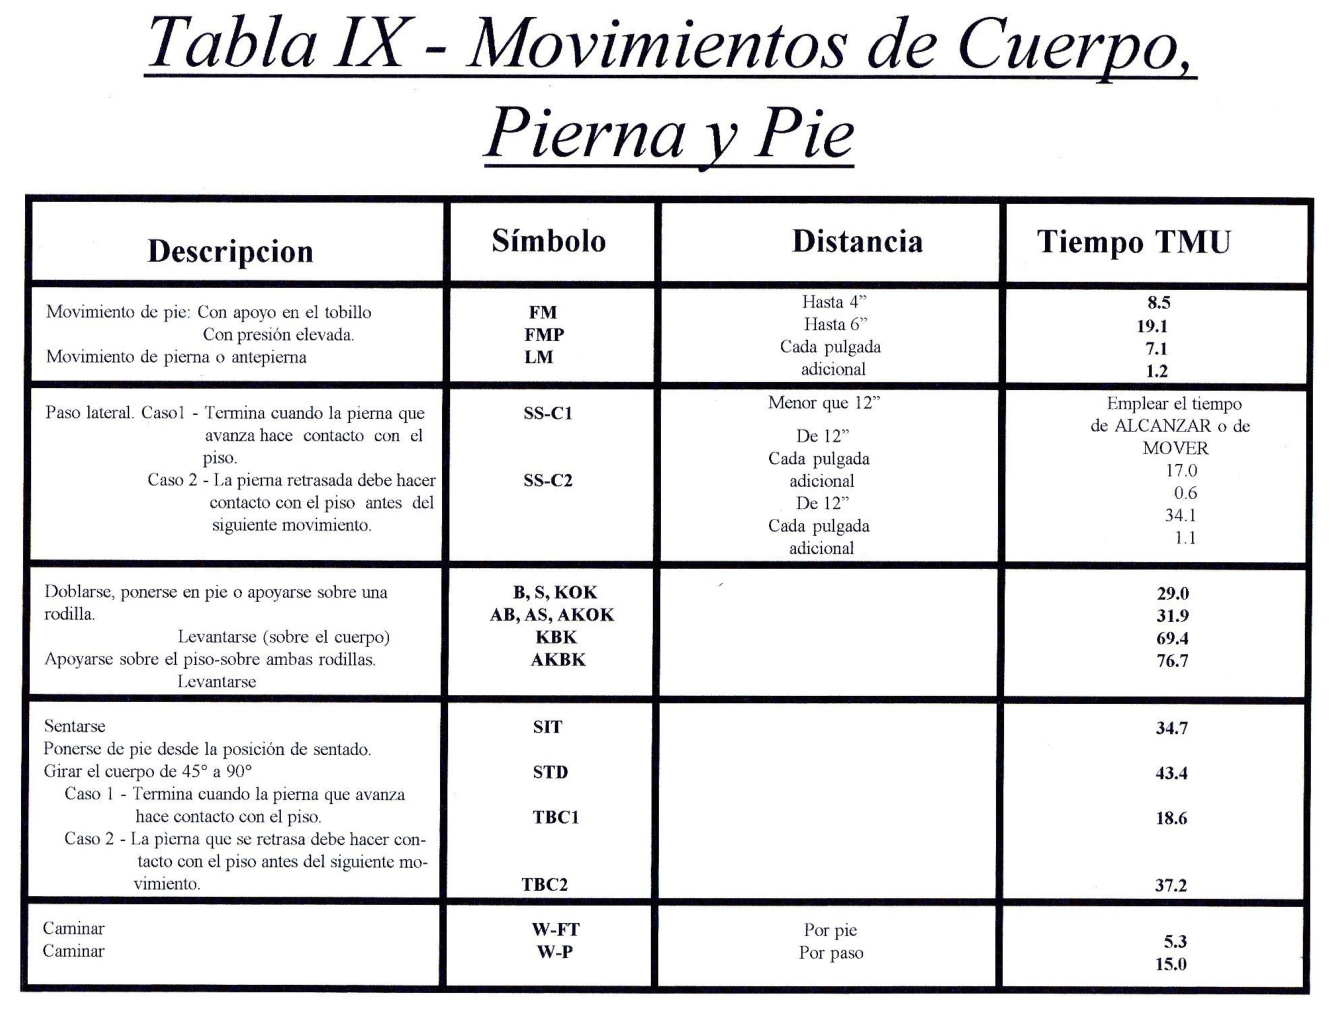
\includegraphics[scale=0.35]{3/Img/tabla9MovimientosDeCuerpoPiernaYPie.pdf}
        \caption{Valores estándar del Therblig Movimientos de Cuerpo, Pierna y Pie.}
        \label{fig:tabla9MovimientosDeCuerpoPiernaYPie}
    \end{figure}
    % 
    % 
    \begin{figure}[H]
        \centering
        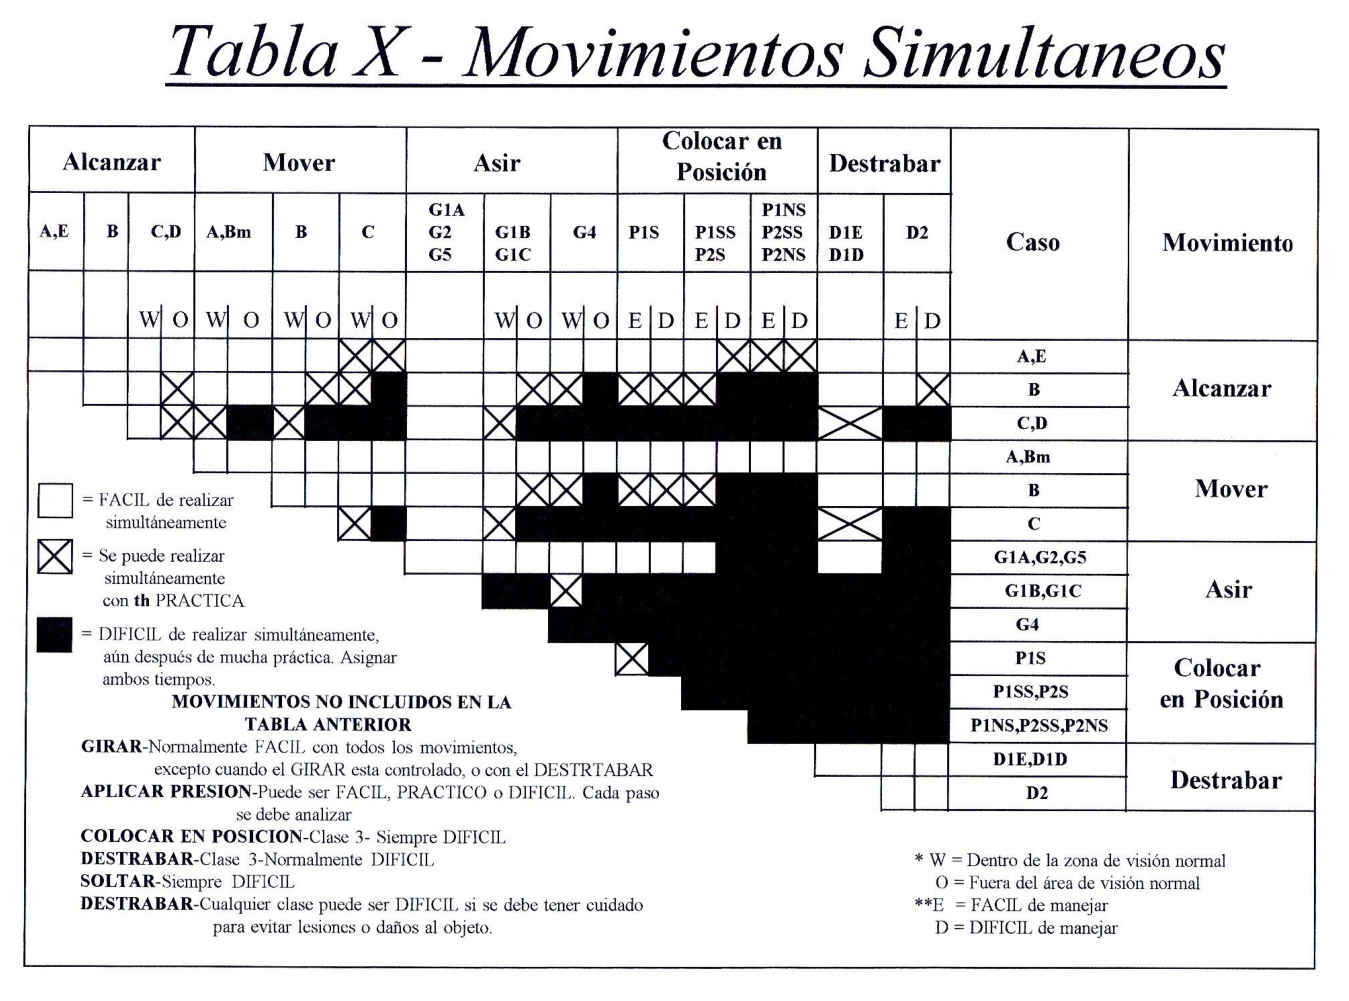
\includegraphics[scale=0.35]{3/Img/tabla10MovimientosSimultaneos.pdf}
        \caption{Movimientos Simultáneos.}
        \label{fig:tabla10MovimientosSimultaneos}
    \end{figure}
    % 
    % 
    \cite{STP}
    % 
    % 
    \subsubsection{Desarrollo del muestreo del trabajo}
    
    El muestreo del trabajo lo podemos considerar como una herramienta para disminuir el costo que se presenta en el estudio continuo del tiempo.
    Utilizando el muestreo del trabajo reducimos el costo, pero se presenta el problema de: Obtener una muestra representativa.
    El muestreo de ocurrencias de tiempos se empleó por primera vez a principios de los años treinta por Tippett (1934) en la industria textil británica. Fue introducido en EUA en 1940 con el nombre de proporción de demoras y se le conoce también como muestreo de trabajo.
    El estudio de tiempos convencional (una película) es una muestra continua de n ciclos (suponiendo que la distribución estadística es normal). El estudio de tiempos no convencional hay huecos entre las lecturas de muestreo; es una muestra discreta (suponiendo que la distribución estadística es binomial).
    Una muestra pequeña ofrece un costo bajo de información; pero se corre un gran riesgo de que la muestra no sea representativa de la población.
    Por otro lado, una muestra grande tiene un costo elevado de información; pero disminuye el riesgo de que la muestra no sea representativa de la población.
    La determinación del porcentaje de tiempo productivo es probablemente el paso más importante en todo el procedimiento de medición del trabajo. También es el paso más sujeto a críticas, ya que está basado en por completo en la experiencia, capacitación y juicio del analista que lo realizará. \cite{Muestreodetrabajo}
    % 
    % 
    Distribución uniforme discreta
     La media de la variable aleatoria discreta (X) es:
        \begin{equation}
             \mu_x=\dfrac{b+a}{2}
        \end{equation}
        
        La desviación estándar de X es:
        \begin{equation}
        \sigma_x=\sqrt{\dfrac{(b-a+1)^2-1}{12}}
        \end{equation}
    % 
    % 
    \subsubsection{Corrección por balanceo de procesos}
    
    El balanceo de líneas son metodologías que buscan mediante métodos y acciones equilibrar el efecto de factores que desestabilizan la sucesión de un trabajo.
    Se presenta el problema de determinar el número ideal de operadores a una línea de producción. El balanceo de líneas más elemental sería distribuir las tareas de trabajo de manera uniforme entre las estaciones de producción. Algunos datos que se necesitan para un balanceo de líneas son: los operadores, minutos estándar para llevar a cabo operación, tiempo de espera en base al operador más lento y tiempo estándar.
    La corrección por balanceo de procesos en un ensamble es una técnica utilizada en la gestión de operaciones y producción para optimizar la distribución del trabajo entre las distintas estaciones de una línea de ensamblaje. El objetivo es minimizar el tiempo ciclo y maximizar la eficiencia y productividad del sistema de producción.
    Para la corrección por balanceo de procesos es fundamental iniciar con el análisis de tareas; determinar el tiempo requerido para completar cada tarea (tiempo de ciclo), así como el ritmo de producción necesario para satisfacer la demanda del cliente. Después la asignación de tareas a estaciones de trabajo ajustándolas para equilibrar la carga de trabajo entre todas las estaciones. Probar el nuevo esquema de balanceo en la línea de producción y observar los resultados. Finalmente Recoger datos de rendimiento y realizar ajustes continuos para mejorar el balanceo de la línea.\cite{Balanceodelíneas} 
    % 
    %  
    \subsubsection{Datos estándar continuos y discretos}
    
    Los datos discretos sólo pueden tomar valores determinados. Se trata de datos que se pueden contar y que tienen un número limitado de valores. Suelen presentarse en forma de números enteros. Los datos continuos son datos que adoptan un número ilimitado de valores diferentes porque sus valores no son fijos y que pueden medirse. 
    Para desarrollar datos de tiempo estándar, los analistas debemos distinguir los elementos constantes de las variables. Un elemento constante es aquel cuyo tiempo permanece casi igual ciclo tras ciclo. Por su parte, el tiempo de un elemento variable varía dentro de un intervalo específico de trabajo.
    En los elementos constantes de las variables en el proyecto integrador tenemos que como elemento constante sería iniciar la máquina y como elemento variable mover el potenciómetro, la velocidad de colocar los pines.
    En las empresas los datos estándares nos permiten establecer tiempos estándar precisos antes de que se realice un trabajo. Se puede estimular los costos, obtener presupuestos, tener una producción equilibrada y realizar ajustes dentro de una operación de trabajo y dentro de una empresa.
    Los datos continuos son aquellos que pueden tomar cualquier valor dentro de un rango específico. Una característica es que pueden asumir infinitos valores posibles dentro de un intervalo.
    Los datos discretos son aquellos que sólo pueden tomar valores específicos y distintos. Una característica es que los valores se encuentran en una escala discreta (no hay valores intermedios entre dos puntos específicos).
    Los datos continuos se obtienen a través de mediciones mientras que por su parte los discretos se obtienen mediante conteos.\cite{Datosestándarcontinuosydiscretos}
    % 
    % 
    \subsection{Diseño de la forma más económica de realizar el trabajo}
    
    1. Selección de componentes
    \begin{itemize}
    \item Estandarización: Opta por componentes estándar y de uso común, que suelen ser más económicos y fáciles de adquirir en grandes cantidades.
    \item Proveedores: Negocia precios con varios proveedores para obtener los mejores descuentos por volumen.
    \item Calidad-Costo: Balancea la calidad y el costo, asegurándote de que los componentes más baratos no comprometan la fiabilidad del circuito.
    \end{itemize}
    % 
    % 
    2. Diseño para la Manufacturabilidad
    \begin{itemize}
    \item Simplificación del Diseño: Diseña el circuito de manera que sea fácil y económico de ensamblar, reduciendo el número de componentes y conexiones innecesarias.
    \end{itemize}
    % 
    % 
    3. Automatización del Proceso de Ensamblaje 
    \begin{itemize}
    \item Soldadura Automatizada: Emplea métodos automatizados de soldadura.
    \end{itemize}
    % 
    % 
    4. Optimización del Proceso de Ensamblaje 
    \begin{itemize}
    \item Documentación y Entrenamiento: Proporciona documentación clara y detallada para cada etapa del ensamblaje y entrena al personal adecuadamente para minimizar errores.
    \end{itemize}
    % 
    % 
    5. Control de Calidad y Pruebas 
    \begin{itemize}
    \item Pruebas de Funcionamiento: Realiza pruebas funcionales del circuito electrónico.
    \end{itemize}
    % 
    % 
    \subsection{Normalización de los métodos, materiales, herramientas e instalaciones}
    
    La normalización de los métodos, materiales, herramientas e instalaciones es un proceso esencial en cualquier industria o campo de trabajo que busca estandarizar y optimizar procesos, asegurar la calidad, mejorar la eficiencia y garantizar la seguridad.
    
    1. Métodos. Para normalizar métodos: 
    \begin{itemize}
    \item Documentar los procedimientos actuales.
    \item Identificar las mejores prácticas y áreas de mejora.
    \item Desarrollar procedimientos estándar detallados.
    \item Implementar y capacitar al personal en los nuevos procedimientos.
    \item Revisar y actualizar regularmente los métodos estándar.
    \end{itemize} 
    % 
    % 
    2. Materiales. Para normalizar materiales: 
    \begin{itemize}
    \item Definir las especificaciones técnicas y de calidad para cada material.
    \item Seleccionar proveedores que cumplan con estos estándares.
    \item Establecer un sistema de control de calidad para verificar la conformidad de los materiales.
    \item Revisar y actualizar regularmente las especificaciones y estándares de los materiales.
    \end{itemize} 
    % 
    % 
    3. Herramientas. Para normalizar herramientas: 
    \begin{itemize}
    \item Identificar las herramientas necesarias para cada tarea.
    \item Seleccionar y estandarizar las herramientas más adecuadas.
    \item Implementar programas de capacitación en el uso correcto de las herramientas.
    \item Establecer procedimientos de mantenimiento y reemplazo de herramientas.
    \item Revisar y actualizar regularmente las herramientas estándar utilizadas.
    \end{itemize} 
    % 
    % 
    4. Instalaciones. Para normalizar instalaciones: 
    \begin{itemize}
    \item Evaluar las instalaciones actuales y identificar áreas de mejora.
    \item Diseñar un plan de disposición y uso de las instalaciones basado en principios de eficiencia y seguridad.
    \item Implementar cambios en la disposición y uso de las instalaciones.
    \item Capacitar al personal en el uso adecuado de las instalaciones.
    \item Revisar y actualizar regularmente el diseño y uso de las instalaciones.
    \end{itemize} 
    % 
    % 
    \subsection{Determinación del tiempo estándar para que una persona competente realice el trabajo con marcha normal}
    
    \begin{itemize}
    \item Selección de la Tarea y del Operario: Seleccionar la tarea específica que se va a estudiar y el operario que realizará la tarea.
    \item Descomposición de la Tarea: Dividir la tarea en elementos básicos que sean fácilmente observables y medibles. Esto facilita el análisis y la medición precisa del tiempo.
    \item Observación y Cronometraje: Realizar múltiples observaciones del operario ejecutando cada uno de los elementos de la tarea. Se utilizan cronómetros para medir el tiempo tomado en cada observación.
    \item Determinación del Tiempo Observado: Registrar los tiempos observados para cada elemento de la tarea.
    \item Calificación de la Marcha: Evaluar la velocidad a la que el operario realiza la tarea en comparación con la marcha normal.
    \item Cálculo del Tiempo Normal: Ajustar el tiempo observado por el factor de calificación de la marcha.
    \item Determinación del Tiempo de Tolerancia: Estimar el tiempo adicional necesario para cubrir necesidades personales, fatiga y retrasos inevitables.
    \item Cálculo del Tiempo Estándar: Incorporar el tiempo de tolerancia al tiempo normal para obtener el tiempo estándar. 
    \end{itemize} 
    % 
    % 
    \section{Resultados y discusión}
    
    \subsection{Desarrollo de la guía de plan de Emergencia}
    
    El objetivo de esta guía es eliminar completamente las emergencias relacionadas con incendios y reducir al mínimo el riesgo de accidentes en el Instituto Tecnológico de Querétaro. Para lograrlo, se capacitará al personal anualmente, asegurando que, en caso de una emergencia, tomen las decisiones más adecuadas para proteger tanto a las personas dentro y fuera de la institución como las instalaciones del instituto. Los datos generales del establecimiento se pueden resumir en la Figura \ref{fig:localizaciónITQ}
    % 
    % 
    \begin{figure}[H]
        \centering
        \includegraphics[scale=0.45]{3/Img/localizaciónITQ.png}
        \caption{Instituto Tecnológico de Querétaro, Av. Tecnológico s/n esq. Gral. Mariano Escobedo. Colonia Centro Histórico C.P. 76000, Querétaro, Querétaro, México. Tel. 442 227 4400, Correo: contacto@itq.edu.mx, Pagina Web: https://querétaro.tecnm.mx/. 
        Cuenta con una	superficie total de 78,271.42 m2 o 842,506.55 Pies2 aproximadamente, así como un total de 5,696 estudiantes aproximadamente tanto de pregrado como posgrado y una planta académica para programas de Licenciaturas de 236 docentes y para Estudios de posgrado 6 docentes, dando un total de 242 docentes, Dicho instituto tiene como director al Ing. Ramón Soto Arriola.}
        \label{fig:localizaciónITQ}
    \end{figure}
    % 
    % 
    Véase también la figura \ref{fig:croquis interno} donde se muestra las medidas del edificio C y del salón C07 del Tecnológico Nacional de México Campus Querétaro donde se llevó a cabo el trabajo de investigación.
    % 
    % 
    \begin{figure}[H]
        \centering
        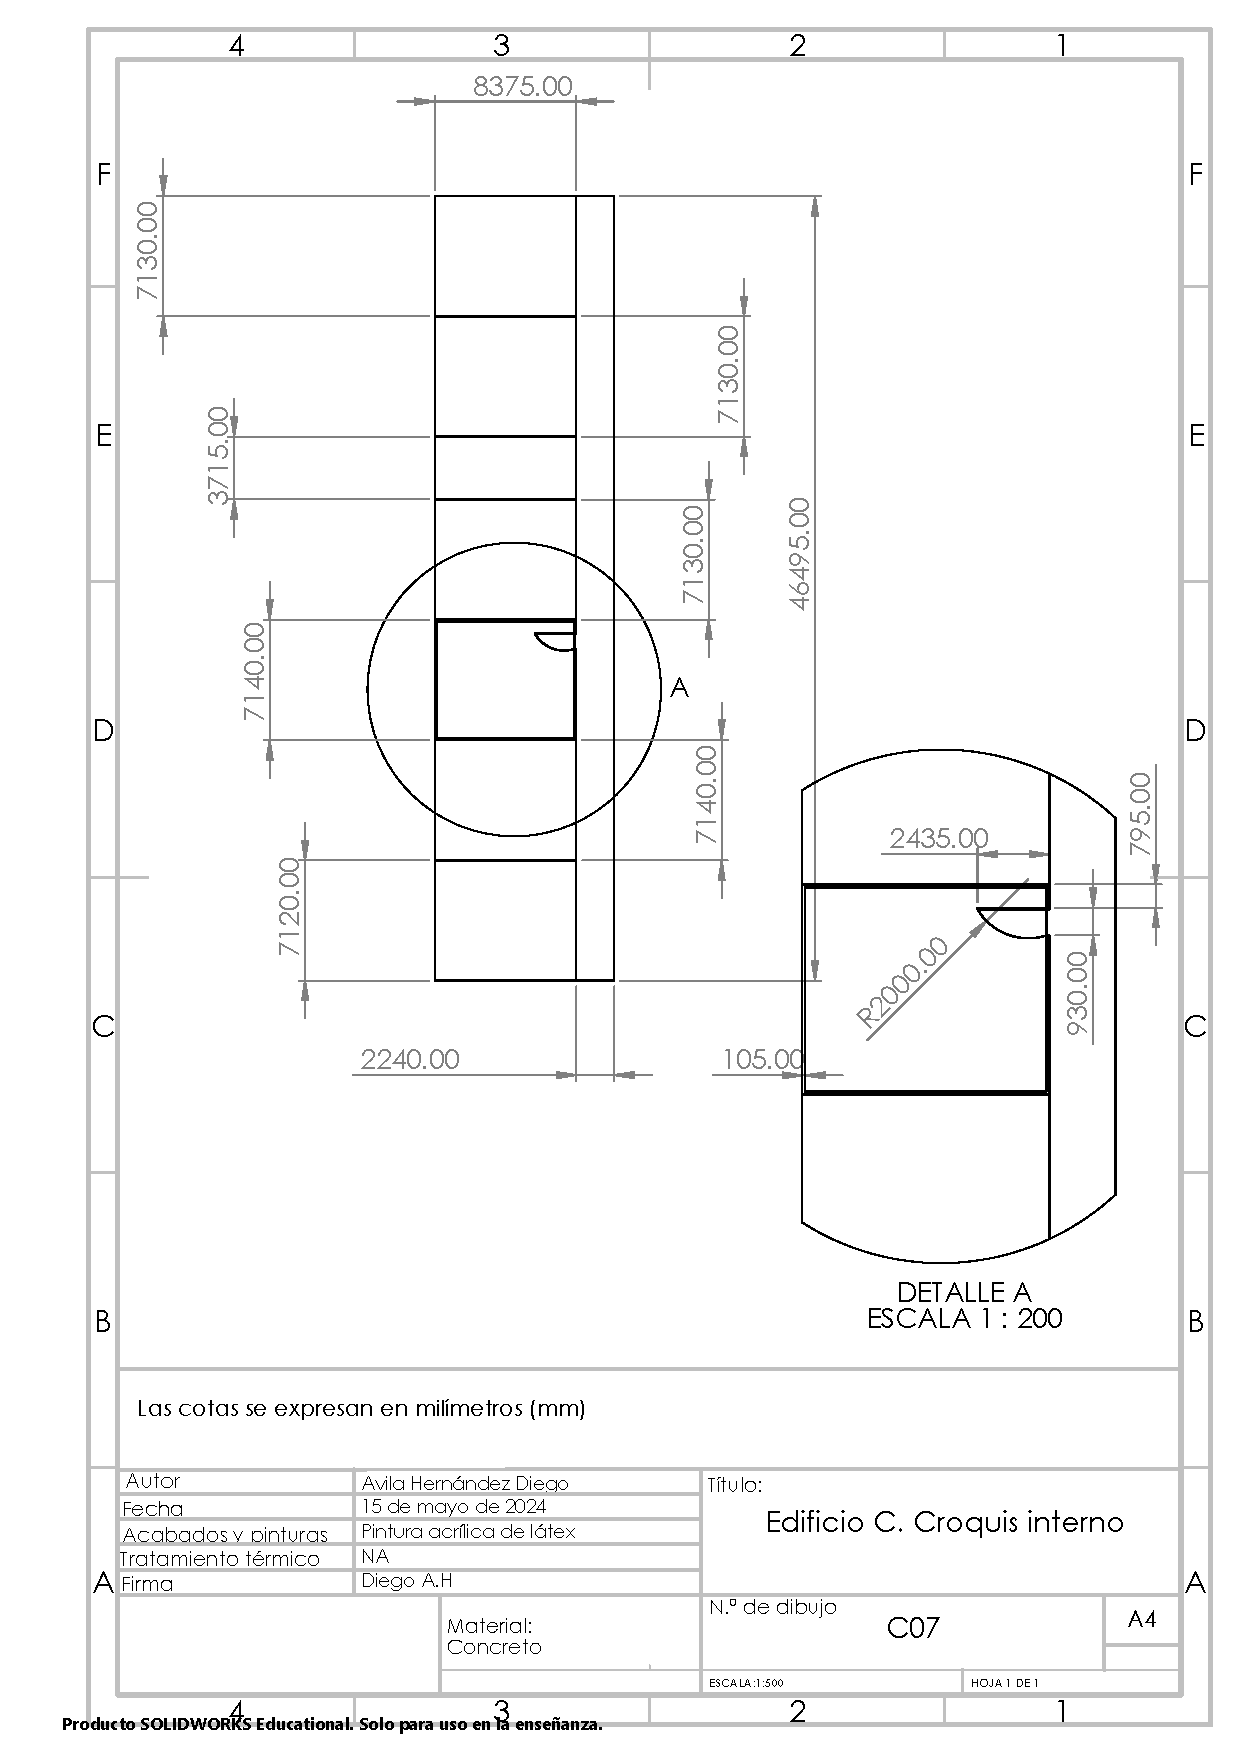
\includegraphics[scale=0.4]{3/Img/croquisInterno2.pdf}
        \caption{Edificio C salón C07: croquis interno del área de trabajo.} 
        \label{fig:croquis interno}
    \end{figure}
    % 
    % 
    \subsubsection{Identificación del riesgo}
    
    La identificación de riesgos es un componente crucial en la gestión de proyectos, empresas, y procesos organizativos. Se refiere al proceso de detectar y documentar los posibles eventos, condiciones o acciones que podrían afectar negativamente el logro de los objetivos establecidos.Estamos dedicados a implementar diariamente un programa interno de prevención de riesgos. También valoramos la retroalimentación de nuestros clientes internos y externos sobre los riesgos que surgen en las actividades cotidianas. Analizamos cada riesgo interno y los clasificamos en un rango para determinar la prioridad de las acciones a tomar. Véase el diagrama \ref{fig:diagrama}
    % 
    % 
    \begin{figure}[H]
        \centering
        \includegraphics[trim = {38mm 160mm 38mm 10mm},clip,scale=0.6]{3/Img/diagramaParaLaIdentificaciónDeRiesgos.pdf}
        \caption{Diagrama para la identificación de riesgos y acciones}
        \label{fig:diagrama}
    \end{figure}
    % 
    % 
    \subsubsection{Riesgos internos}
    
    El riesgo es la posibilidad de que ocurra un evento o acción que tenga consecuencias negativas o desfavorables. El riesgo interno se refiere a los riesgos que se originan dentro de una organización y que pueden afectar negativamente su desempeño, operaciones y objetivos. Estos riesgos son controlables hasta cierto punto por la propia organización, ya que provienen de sus procesos internos, estructuras, personal y sistemas.
    Véase la tabla \ref{fig:tabla de riesgos} 
    % 
    %
    \begin{figure}[H]
        \centering
        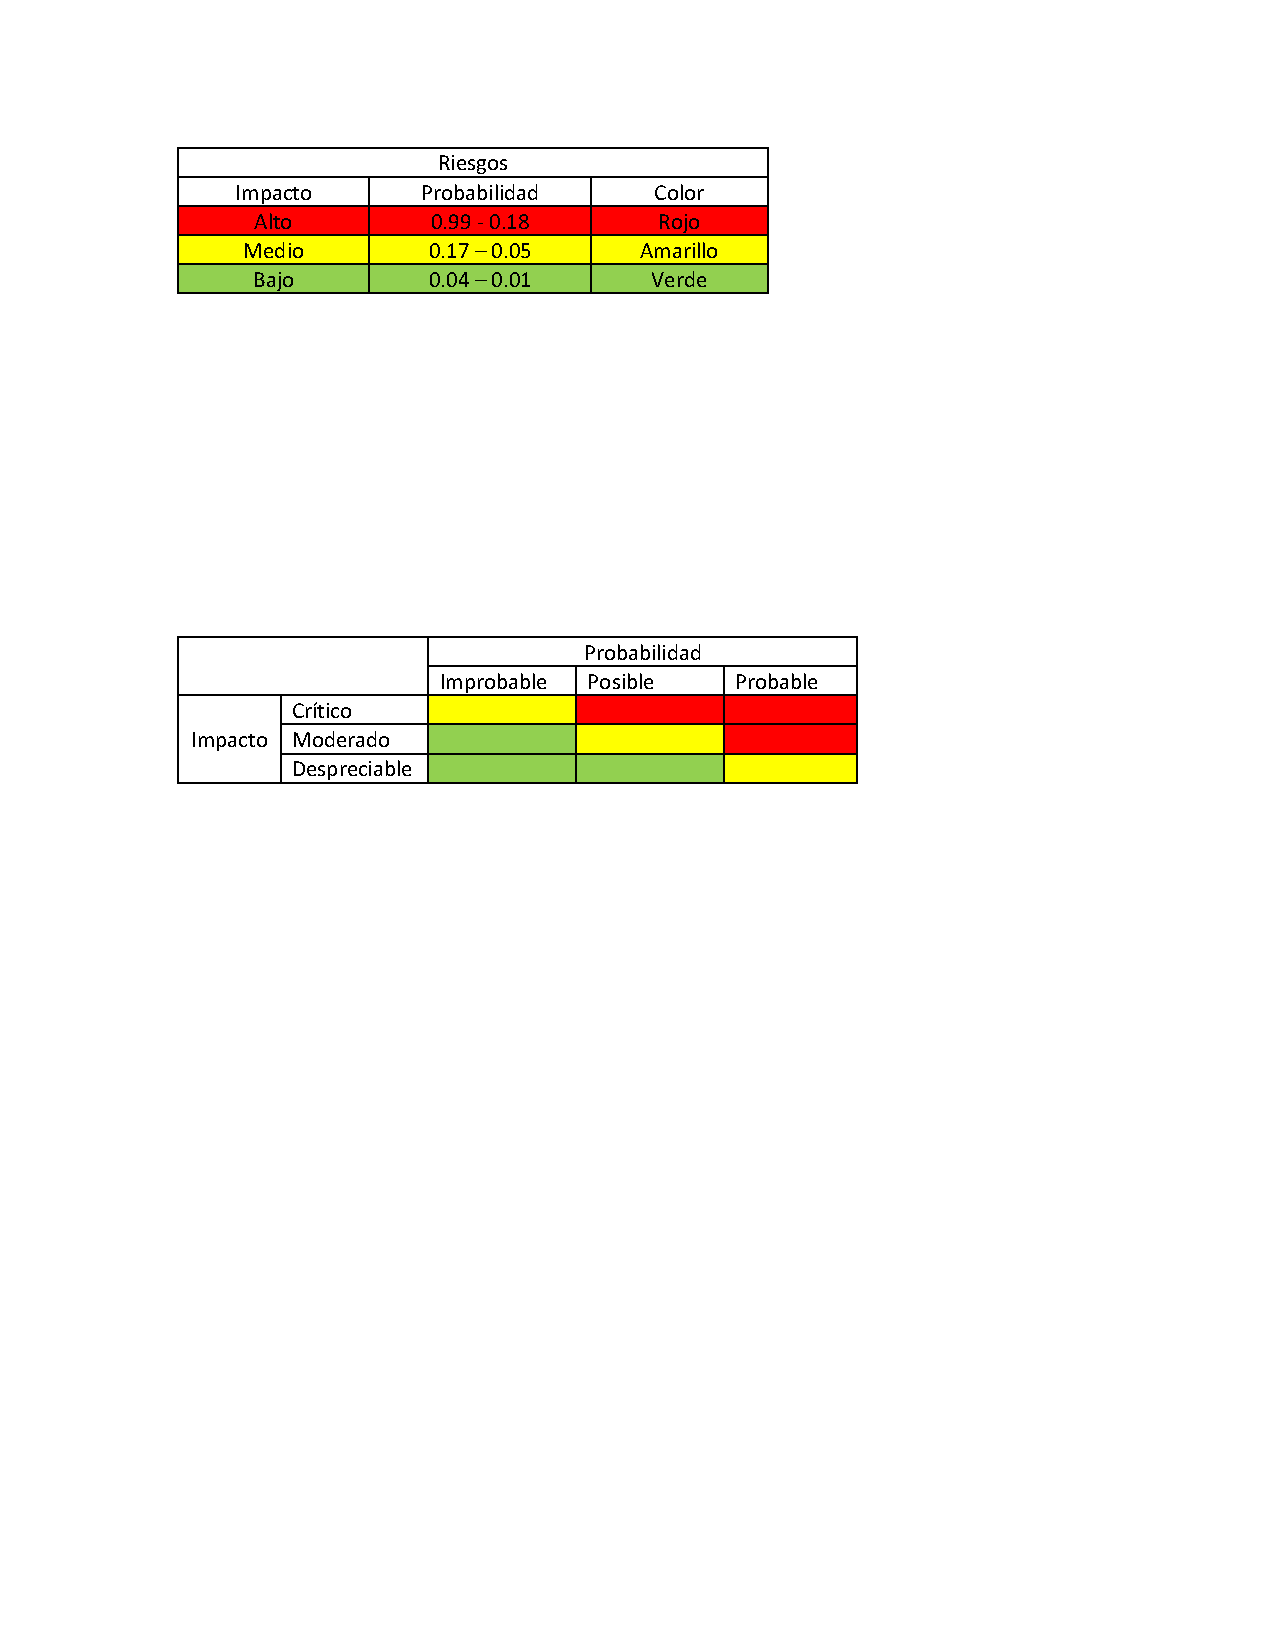
\includegraphics[trim = {10mm 220mm 10mm 10mm},clip,scale=0.6]{3/Img/tablaDeRiesgosConDiferentesNiveles.pdf}
        \caption{Tabla de riesgos con diferentes niveles y colores para distinguir la gravedad y acciones}
        \label{fig:tabla de riesgos}
    \end{figure}
    % 
    %
    Véase la tabla de riesgos \ref{fig:tabla de riesgos internos}
    % 
    %
    \begin{figure}[H]
        \centering
        \includegraphics[trim = {0mm 70mm 0mm 0mm},clip,scale=0.4]{3/Img/descripciónDeRiesgosInternos.pdf}
        \caption{Tabla de riesgos que se pueden presentar por parte del área de trabajo y también por las actividades que realiza el operador} 
        \label{fig:tabla de riesgos internos}
    \end{figure}
    % 
    %
    \subsubsection{Riesgos externos}
    
    Los riesgos externos son factores o eventos que pueden afectar negativamente a una organización pero que están fuera de su control directo. A diferencia de los riesgos internos, que provienen de dentro de la organización y pueden ser gestionados directamente, los riesgos externos son originados por fuerzas y eventos externos al entorno empresarial. Estos riesgos pueden tener un impacto significativo en las operaciones, la reputación y la viabilidad a largo plazo de una organización.Véase la tabla \ref{fig:tabla de riesgos externos}
    % 
    %
    \begin{figure}[H]
        \centering
        \includegraphics[trim = {0mm 70mm 0mm 0mm},clip,scale=0.4]{3/Img/descripciónDeRiesgosExternos.pdf}
        \caption{Tabla de riesgos que se pueden presentar dentro y fuera del campus} 
        \label{fig:tabla de riesgos externos}
    \end{figure}
    % 
    %
    \subsubsection{Programa de actividades de prevención y auxilio}
    
    Este programa tiene como objetivo principal identificar riesgos potenciales internos u externos, establecer medidas preventivas y diseñar protocolos eficientes de respuesta ante emergencias.
    % 
    % 
    \subsubsection{Plan de acción}
    
    Un plan de acción de riesgos en el ITQ es una estrategia integral diseñada para identificar, evaluar y mitigar los riesgos potenciales internos u externos que podrían afectar negativamente sus operaciones, activos, reputación y la seguridad de su comunidad. Véase las  tablas \ref{fig:descripciónAccionesDeUnRiesgoInterno} \ref{fig:descripciónAccionesDeUnRiesgoExterno}
    % 
    %
    \begin{figure}[H]
        \centering
        \includegraphics[trim = {0mm 50mm 0mm 0mm},clip,scale=0.4]{3/Img/descripciónAccionesDeUnRiesgoInterno.pdf}
        \caption{Descripción de las acciones anticipadas y correctivas ante un riesgo interno.} 
        \label{fig:descripciónAccionesDeUnRiesgoInterno}
    \end{figure}
    % 
    %
    \begin{figure}[H]
        \centering
        \includegraphics[trim = {0mm 50mm 0mm 0mm},clip,scale=0.4]{3/Img/descripciónAccionesDeUnRiesgoExterno.pdf}
        \caption{Descripción de las acciones anticipadas y correctivas ante un riesgo externo.} 
        \label{fig:descripciónAccionesDeUnRiesgoExterno}
    \end{figure}
    % 
    % 
    \subsubsection{Identificación de capacidades}
    % 
    %
    \begin{figure}[H]
        \centering
        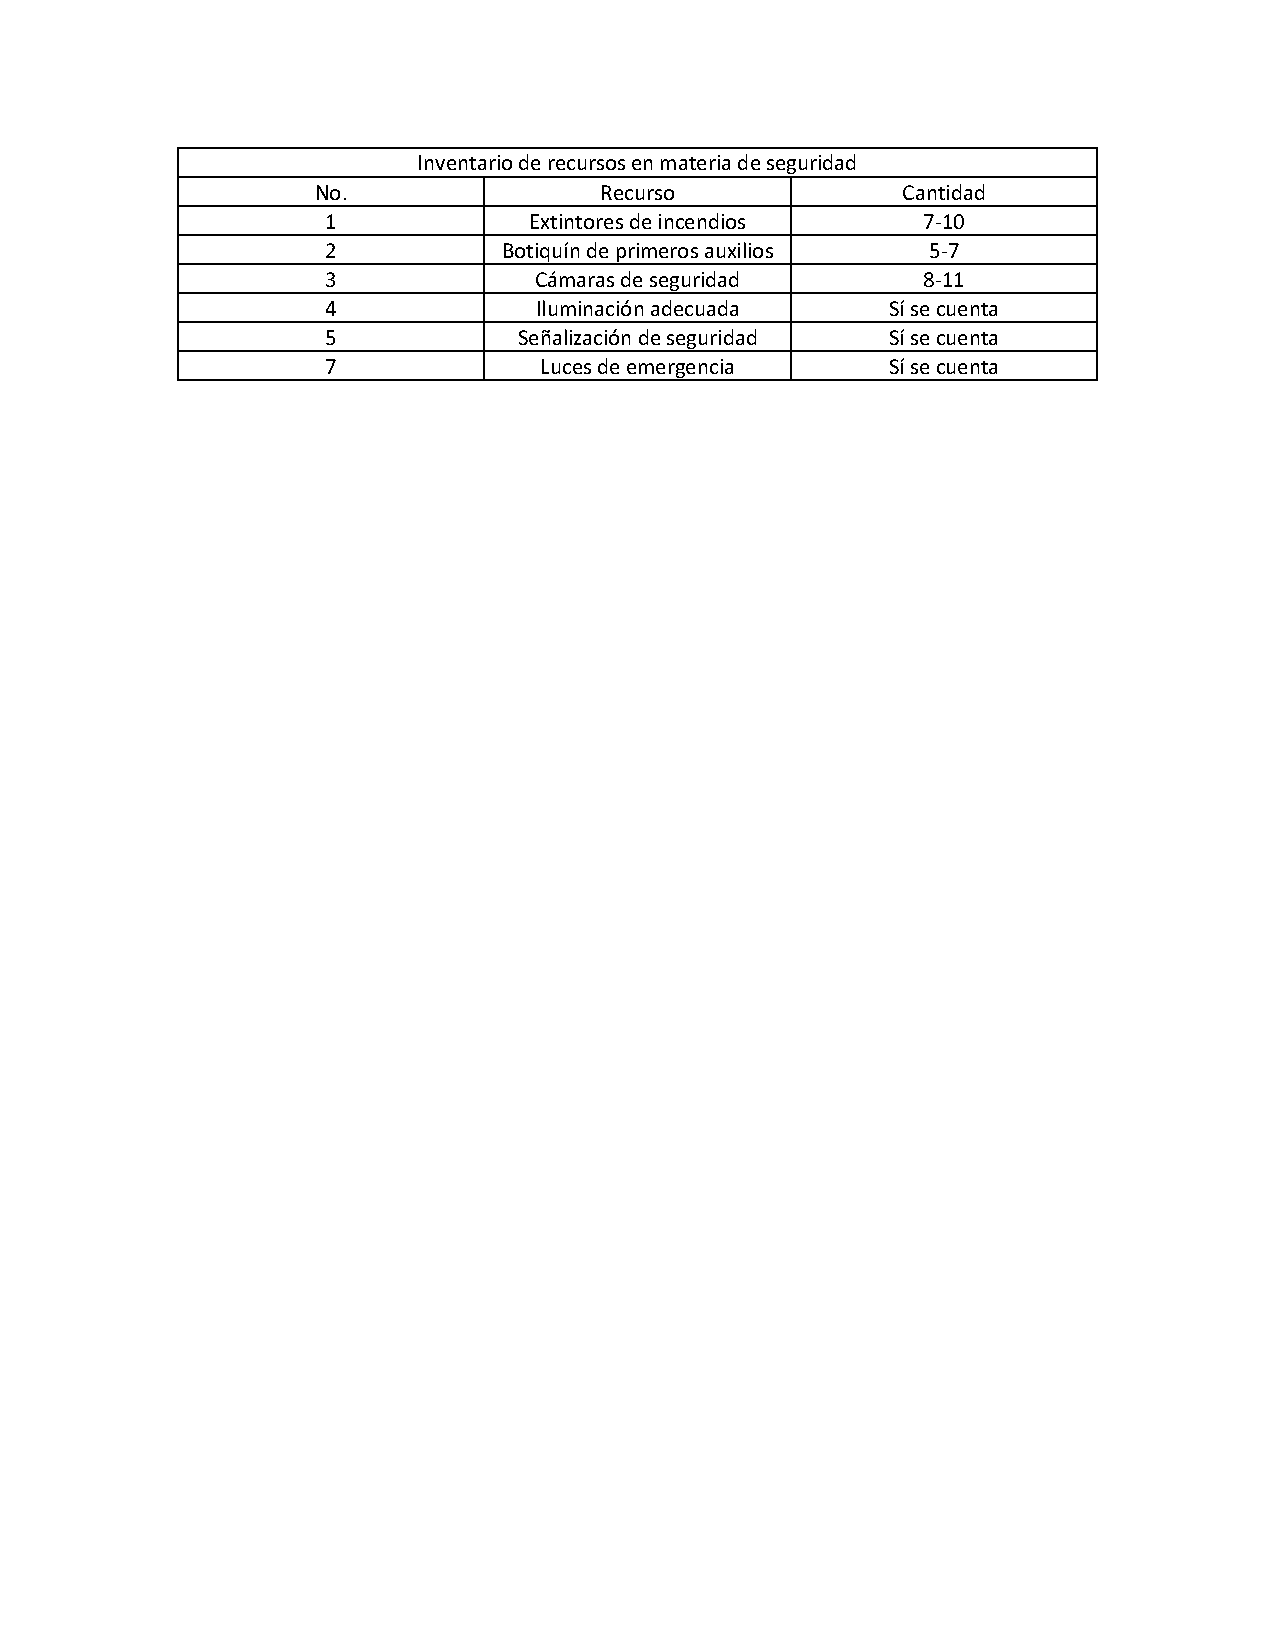
\includegraphics[trim = {0mm 90mm 0mm 20mm},clip,scale=0.4]{3/Img/inventarioDeRecursos.pdf}
        \caption{Recursos en materia de seguridad} 
        \label{fig:Recursos en materia de seguridad}
    \end{figure}
    % 
    % 
    \subsubsection{Plano de localización de recursos}
    % 
    %
    \begin{figure}[H]
        \centering
        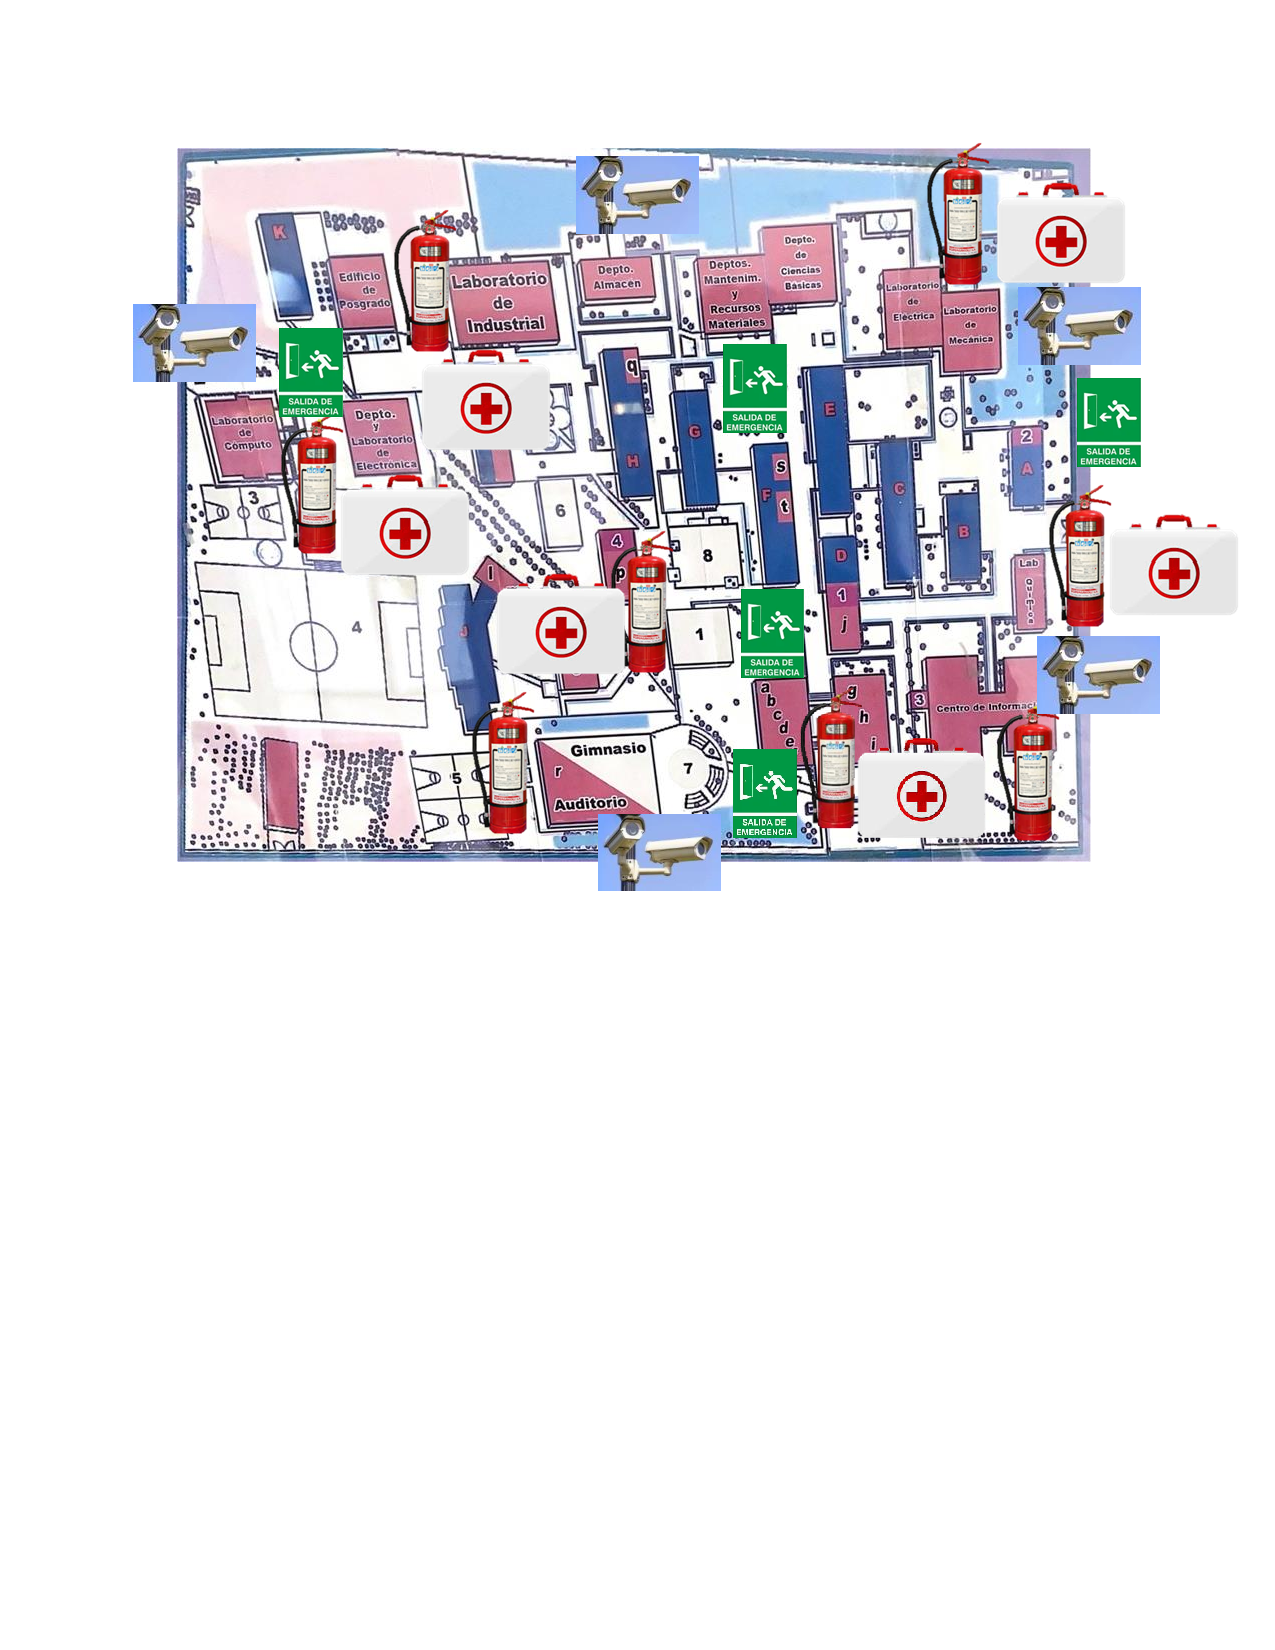
\includegraphics[trim = {30mm 130mm 5mm 21mm},clip,scale=0.5]{3/Img/planoDeEstablecimiento.pdf}
        \caption{Plano del establecimiento de los recursos en materia de seguridad.} 
        \label{fig:Plano de establecimiento}
    \end{figure}
    % 
    % 
    \subsubsection{ Identificación de apoyos externos}
    
    % 
    \begin{figure}[H]
        \centering
        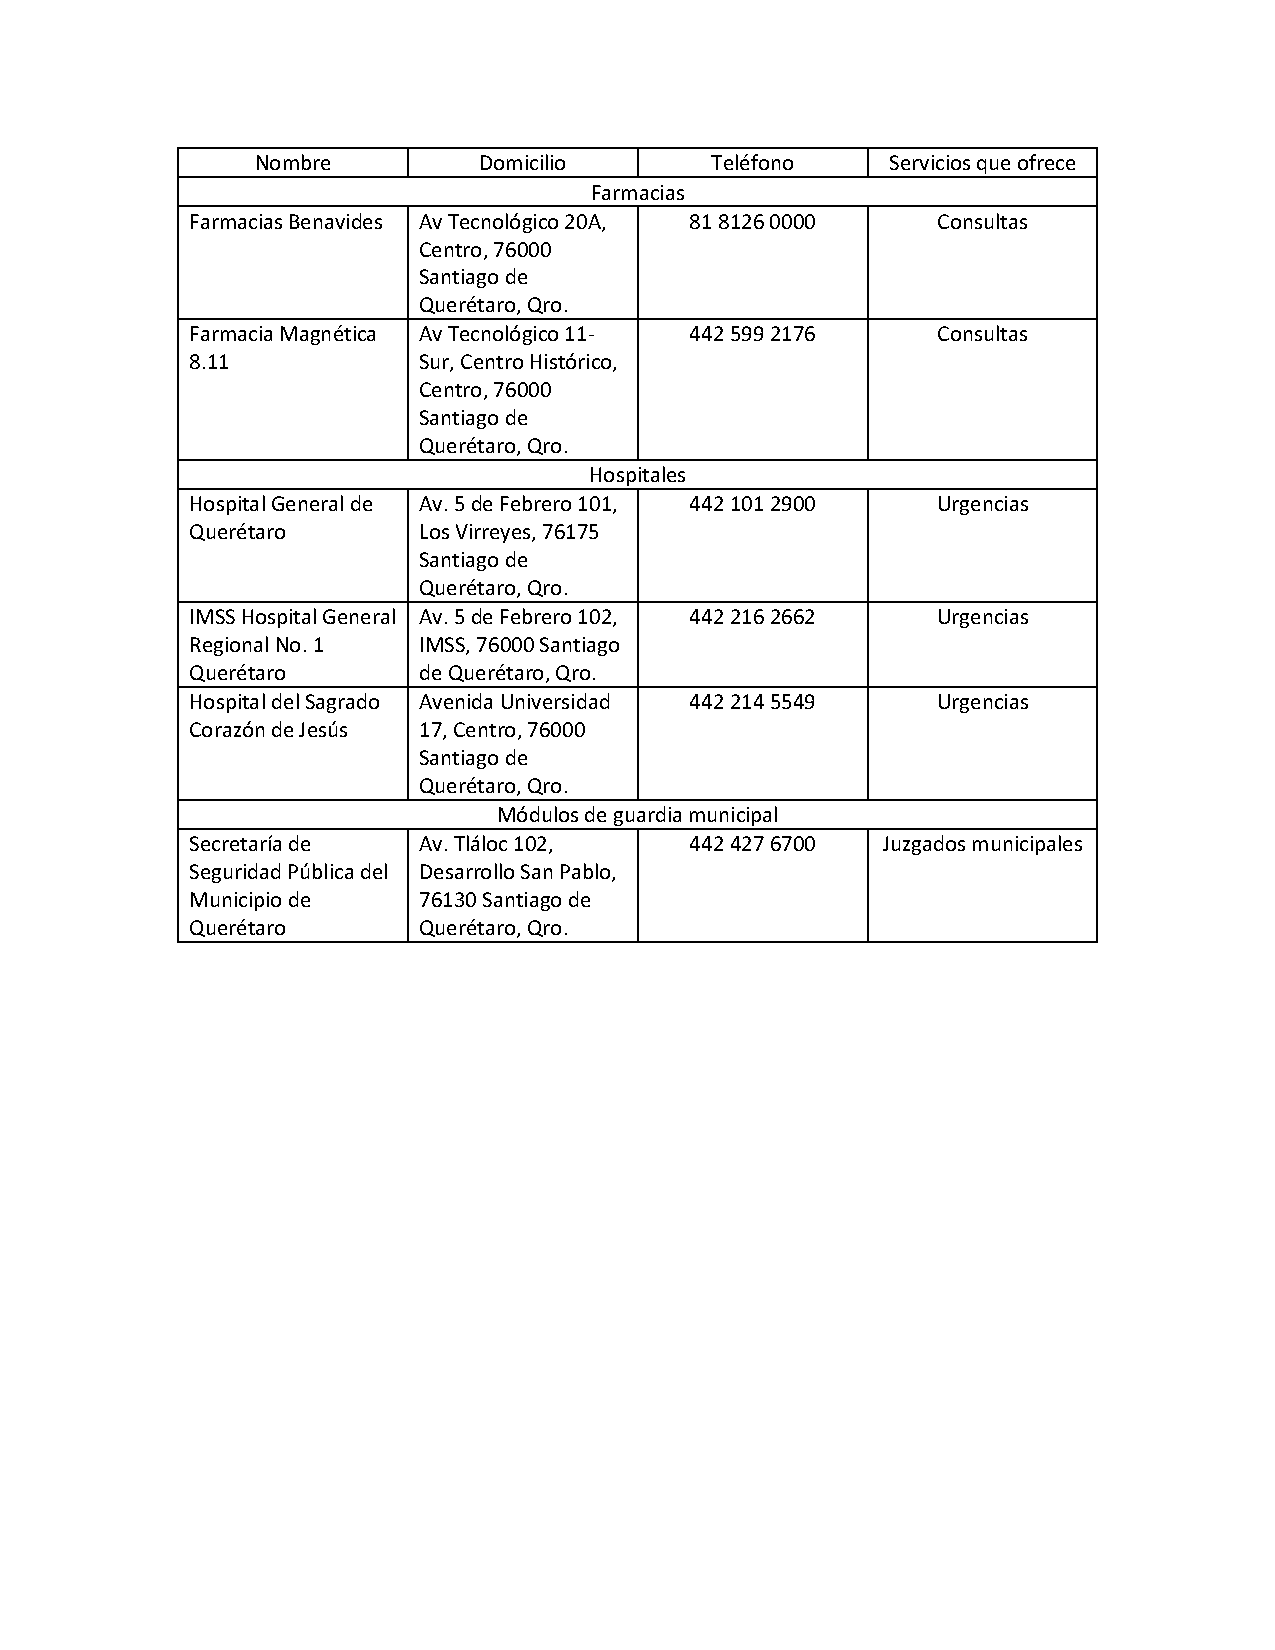
\includegraphics[trim = {20mm 95mm 20mm 20mm},clip,scale=0.5]{3/Img/apoyosExternos.pdf}
        \caption{ Lugares que servirán de apoyo en un situación de emergencia.}
        \label{fig:apoyosExternos}
    \end{figure}
    % 
    % 
    \subsubsection{Identificación de puntos de reunión}
    
    \begin{figure}[H]
        \centering
        \includegraphics[trim = {30mm 130mm 5mm 21mm},clip,scale=0.5]{3/Img/puntosDeReunión.pdf}
        \caption{Zona segura en caso de una evacuación de emergencia.}
        \label{fig:puntosDeReunión}
    \end{figure}
    % 
    % 
    \subsubsection{Brigada de evacuación}
    
    \begin{figure}[H]
        \centering
        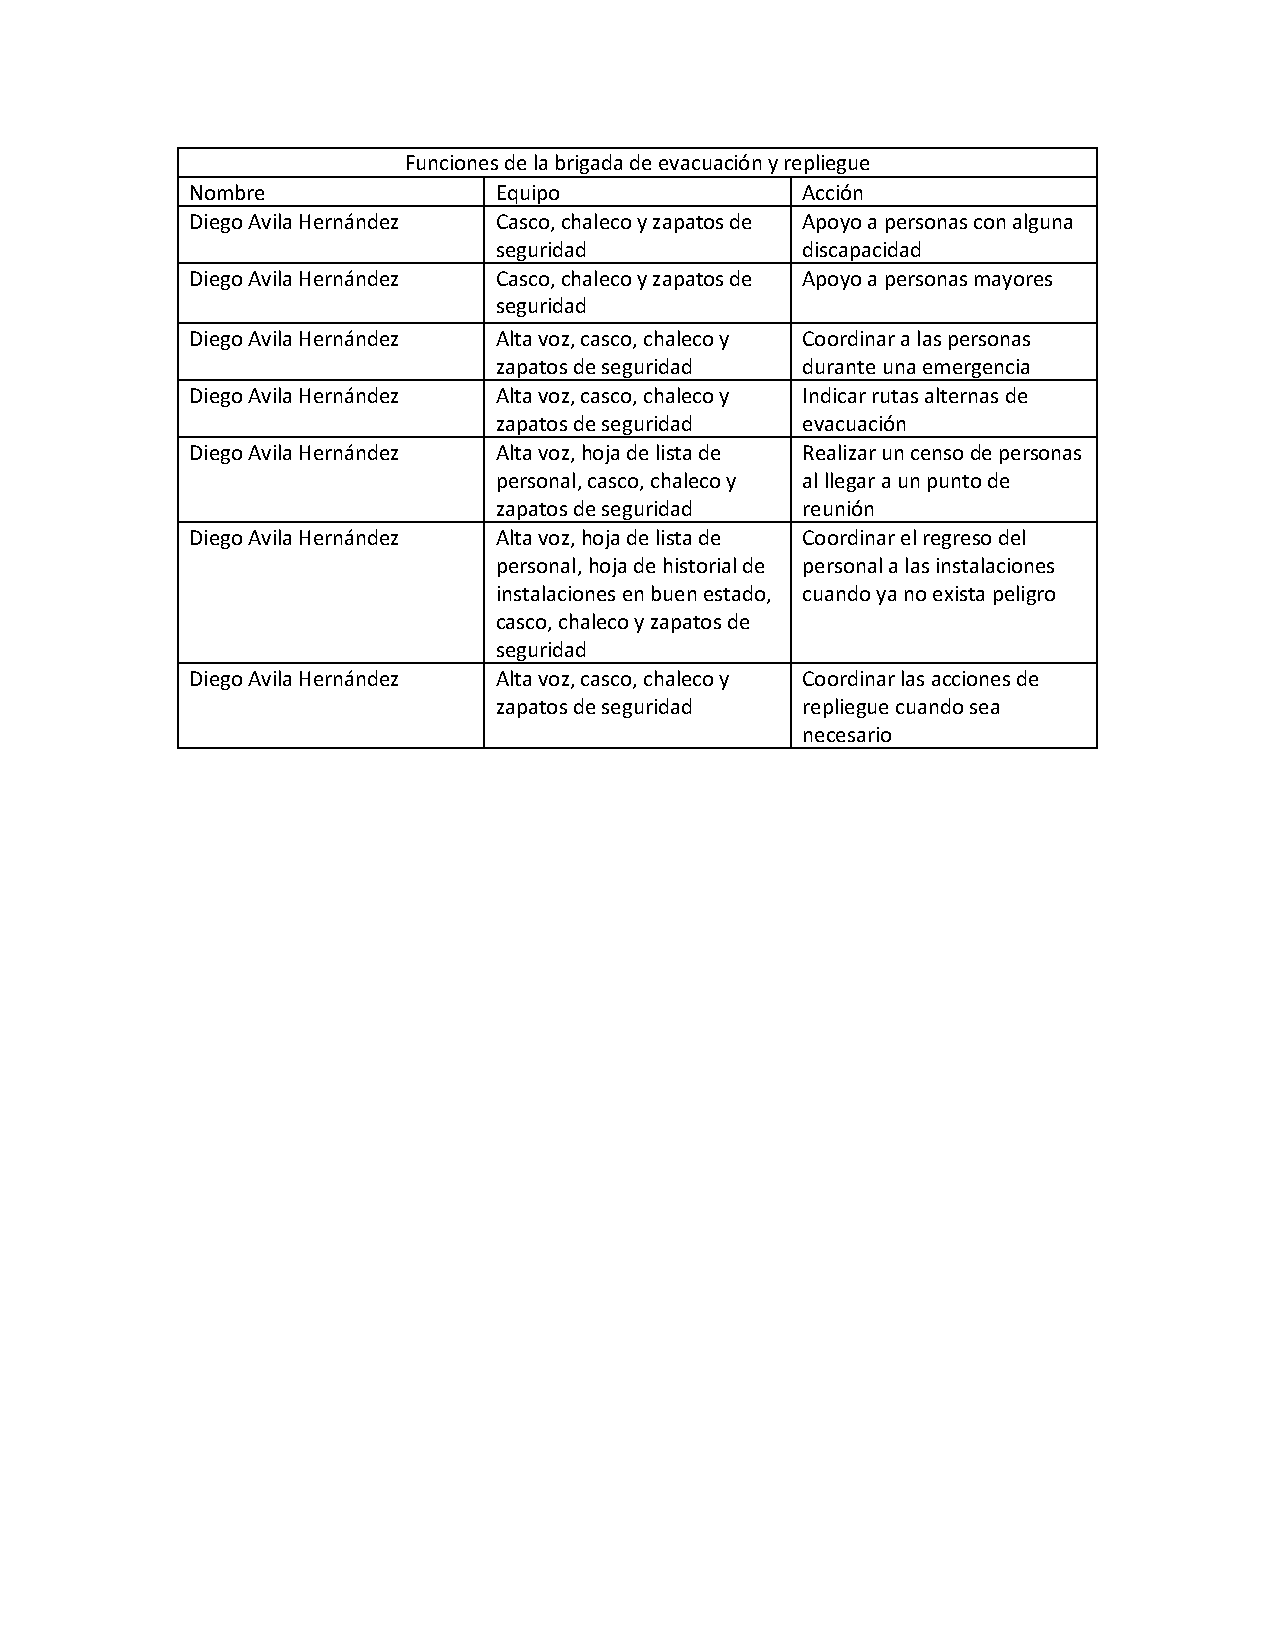
\includegraphics[trim = {20mm 120mm 20mm 25mm},clip,scale=0.5]{3/Img/brigada.pdf}
        \caption{Acciones asignadas a cada integrante del equipo de trabajo en caso de una evacuación de emergencia o repliegue.}
        \label{fig:brigada}
    \end{figure}
    % 
    % 
    \subsubsection{Directorio de telefónicos de emergencia}
    
    Directorio telefónico de instituciones de respuesta a emergencias y otras organizaciones responsables del monitoreo y control de estas situaciones.
    
    \begin{figure}[H]
        \centering
        
\includegraphics[scale=0.65]{3/Img/emergencias911.png}
        \caption{Número único de llamadas de emergencia.}
    \end{figure}
    % 
    % 
    \begin{figure}[H]
        \centering
        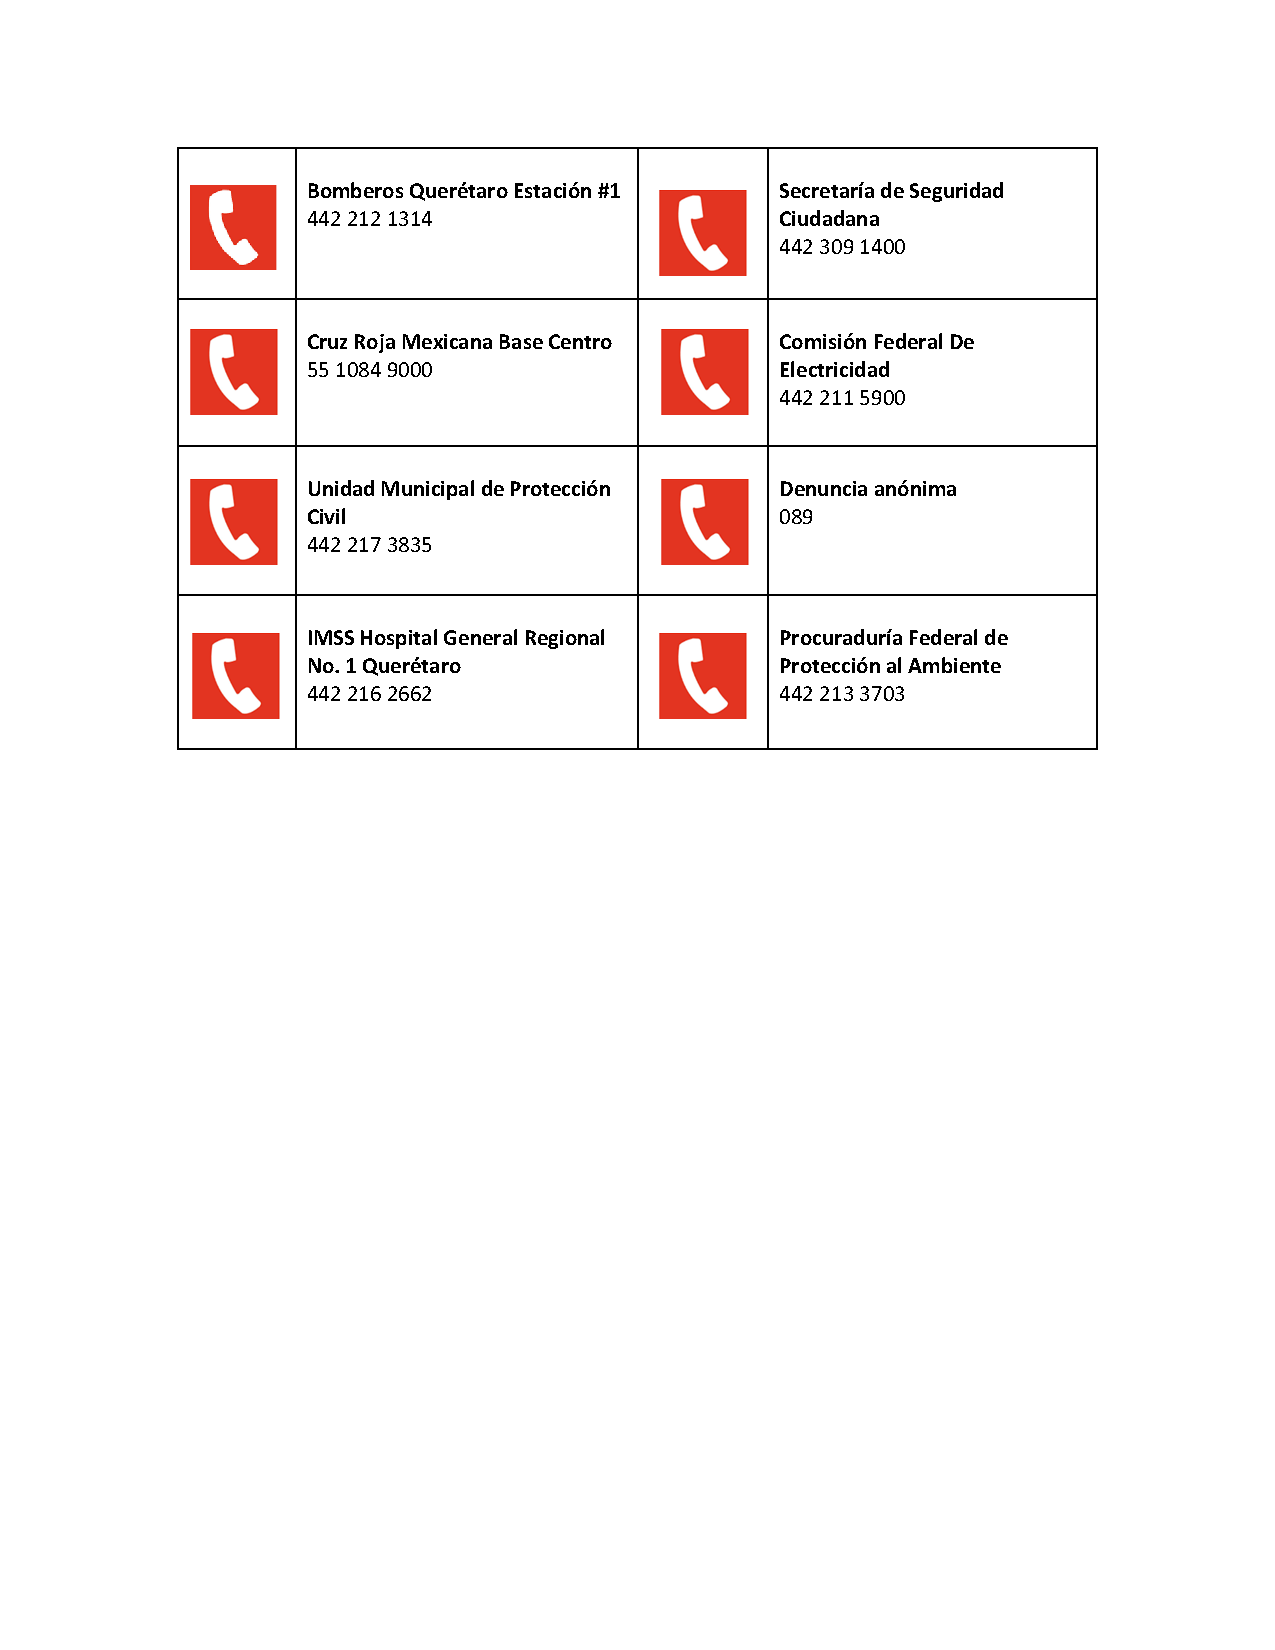
\includegraphics[trim = {20mm 120mm 20mm 25mm},clip,scale=0.5]{3/Img/directorio.pdf}
        \caption{Números de emergencia más próximos a la ubicación del posible riesgo.}
        \label{fig:directorio}
    \end{figure}
    % 
    % 
    \subsection{Análisis de los métodos, materiales, herramientas e instalación utilizada en la ejecución del ensamble de un circuito electrónico}
    
    Véase los materiales que se presentan a continuación:Figura \ref{fig:multicontactoDibujo}.\ref{fig:cableUSB-CDibujo}.\ref{fig:potenciómetroDibujo}.\ref{fig:lcdDibujo}.\ref{fig:móduloAdaptadorLcdDibujo}.\ref{fig:esp32Dibujo}.\ref{fig:protoboardDibujo}.\ref{fig:resistenciaDibujo}.\ref{fig:cableMHDibujo}.\ref{fig:cableMMDibujo}.\ref{fig:tapeteProfesionalOrganizadorDeTrabajoDibujo}. 
    % 
    % 
    \begin{figure}[H]
        \centering
        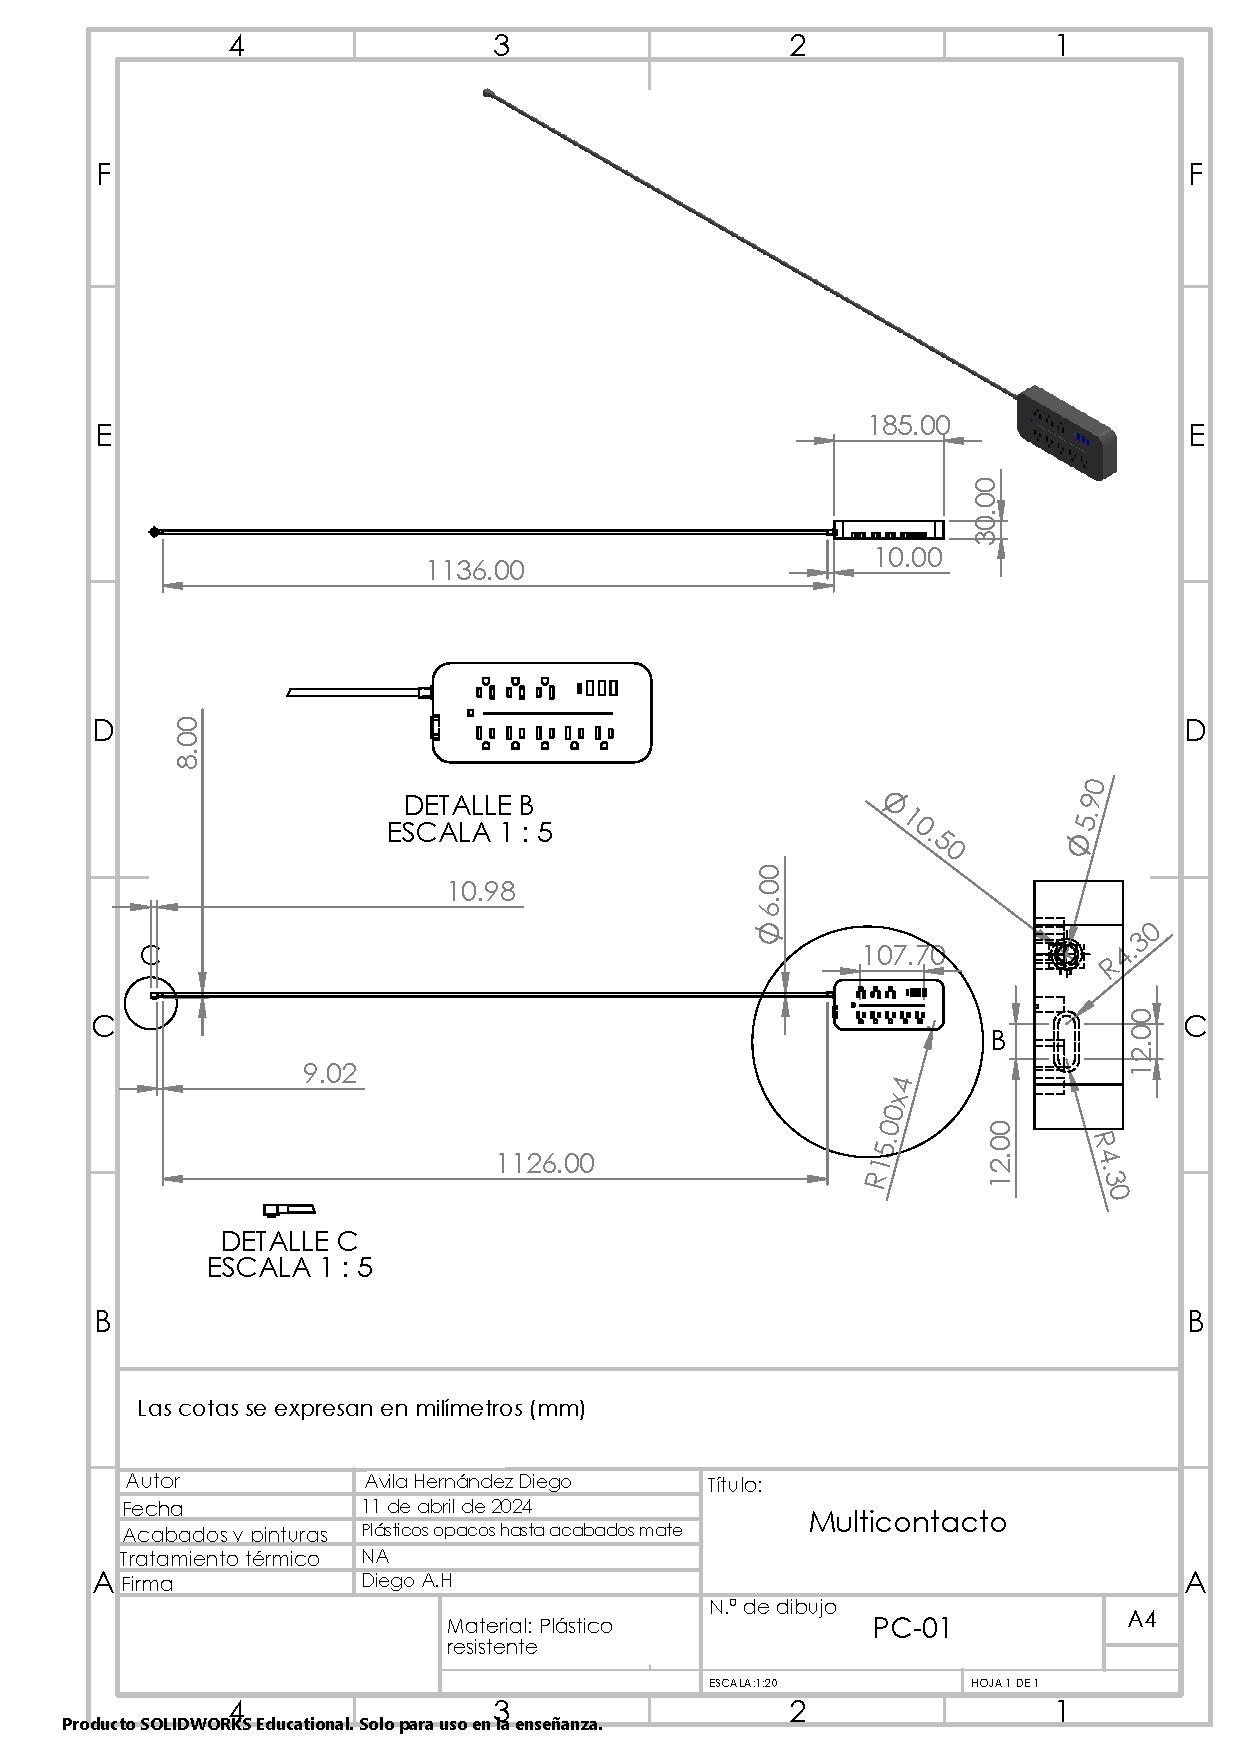
\includegraphics[scale=0.4]{3/Img/multicontactoDibujo.pdf}
        \caption{PC-01 Multicontacto} 
        \label{fig:multicontactoDibujo}
    \end{figure}
    % 
    % 
    \begin{figure}[H]
        \centering
        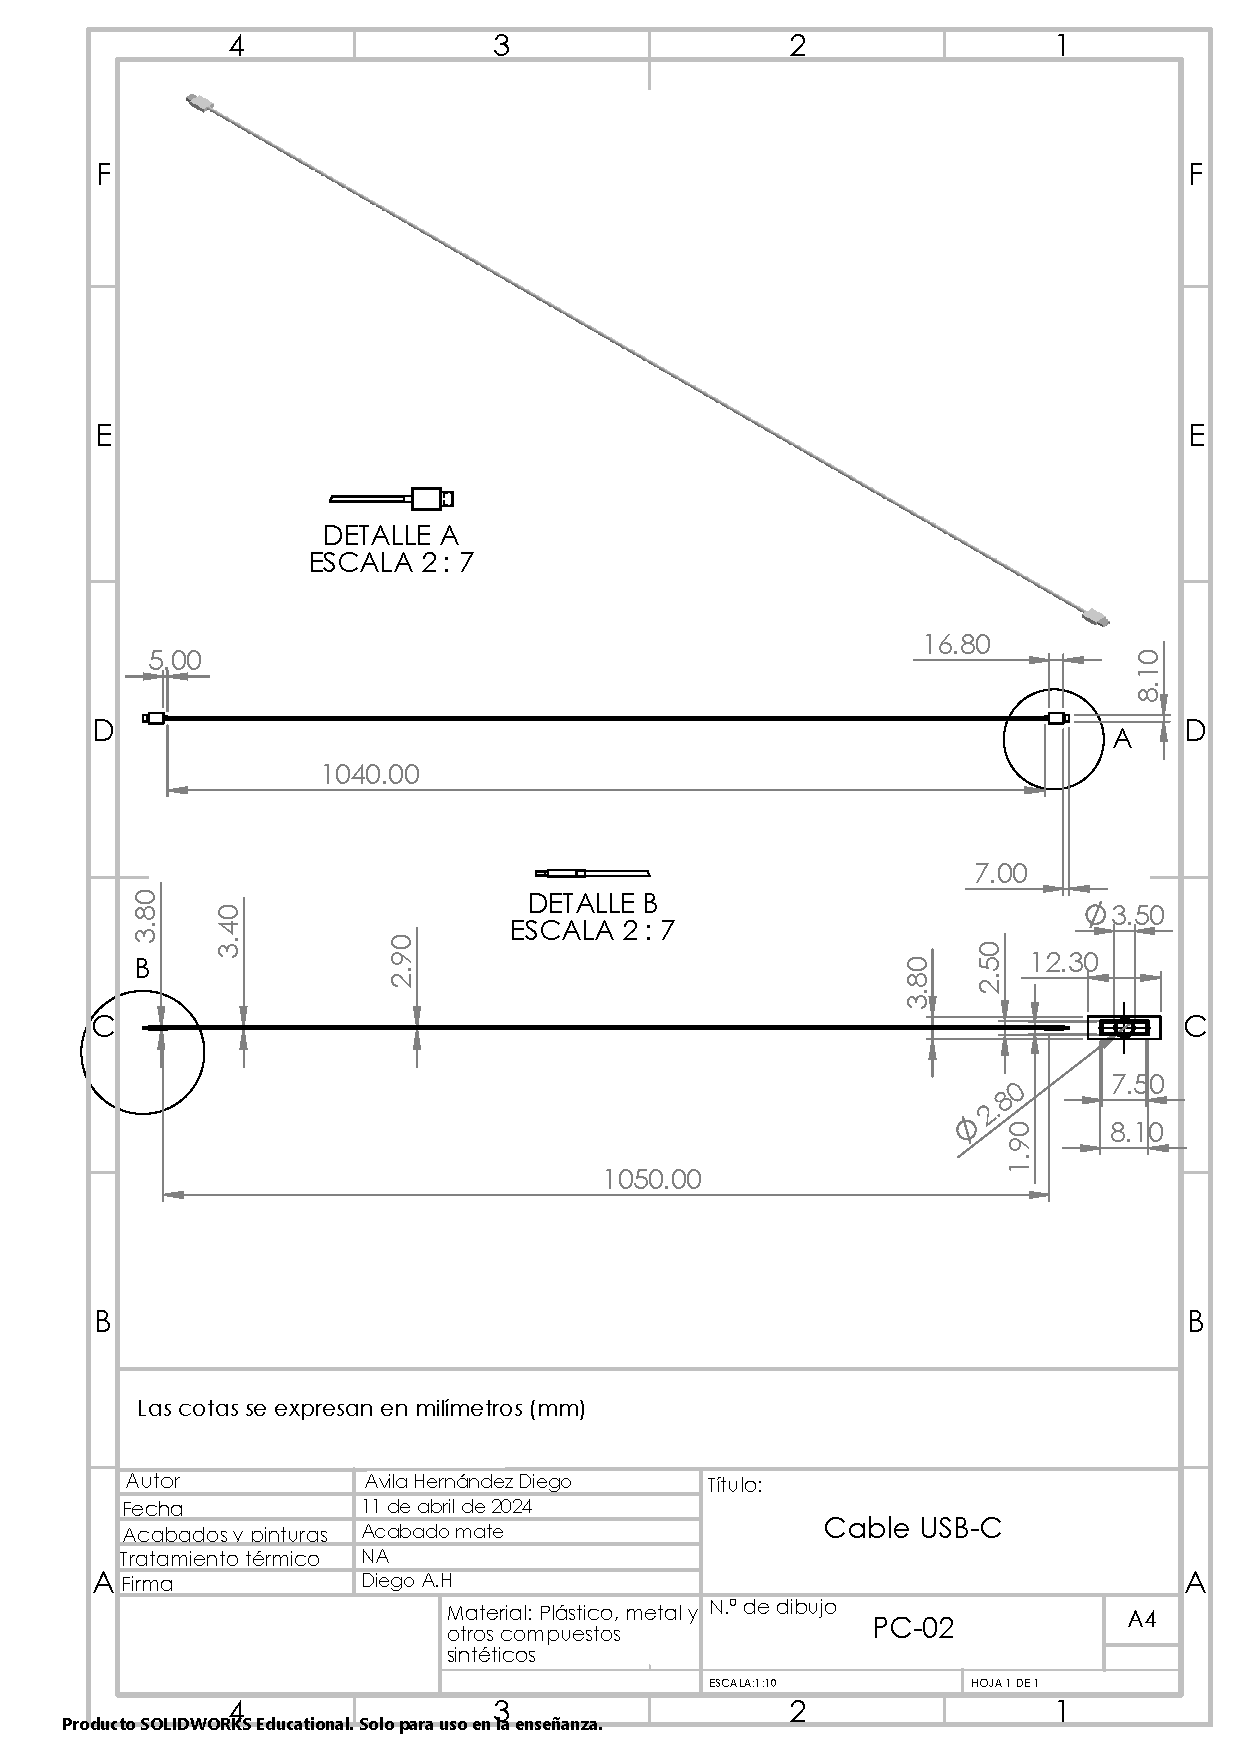
\includegraphics[scale=0.4]{3/Img/cableUSB-CDibujo.pdf}
        \caption{PC-02 Cable USB-C} 
        \label{fig:cableUSB-CDibujo}
    \end{figure}
    % 
    % 
    \begin{figure}[H]
        \centering
        \includegraphics[scale=0.4]{3/Img/potenciómetroDibujo.pdf}
        \caption{PC-03 Potenciómetro 3541H-1-102L 1k} 
        \label{fig:potenciómetroDibujo}
    \end{figure}
    % 
    % 
    \begin{figure}[H]
        \centering
        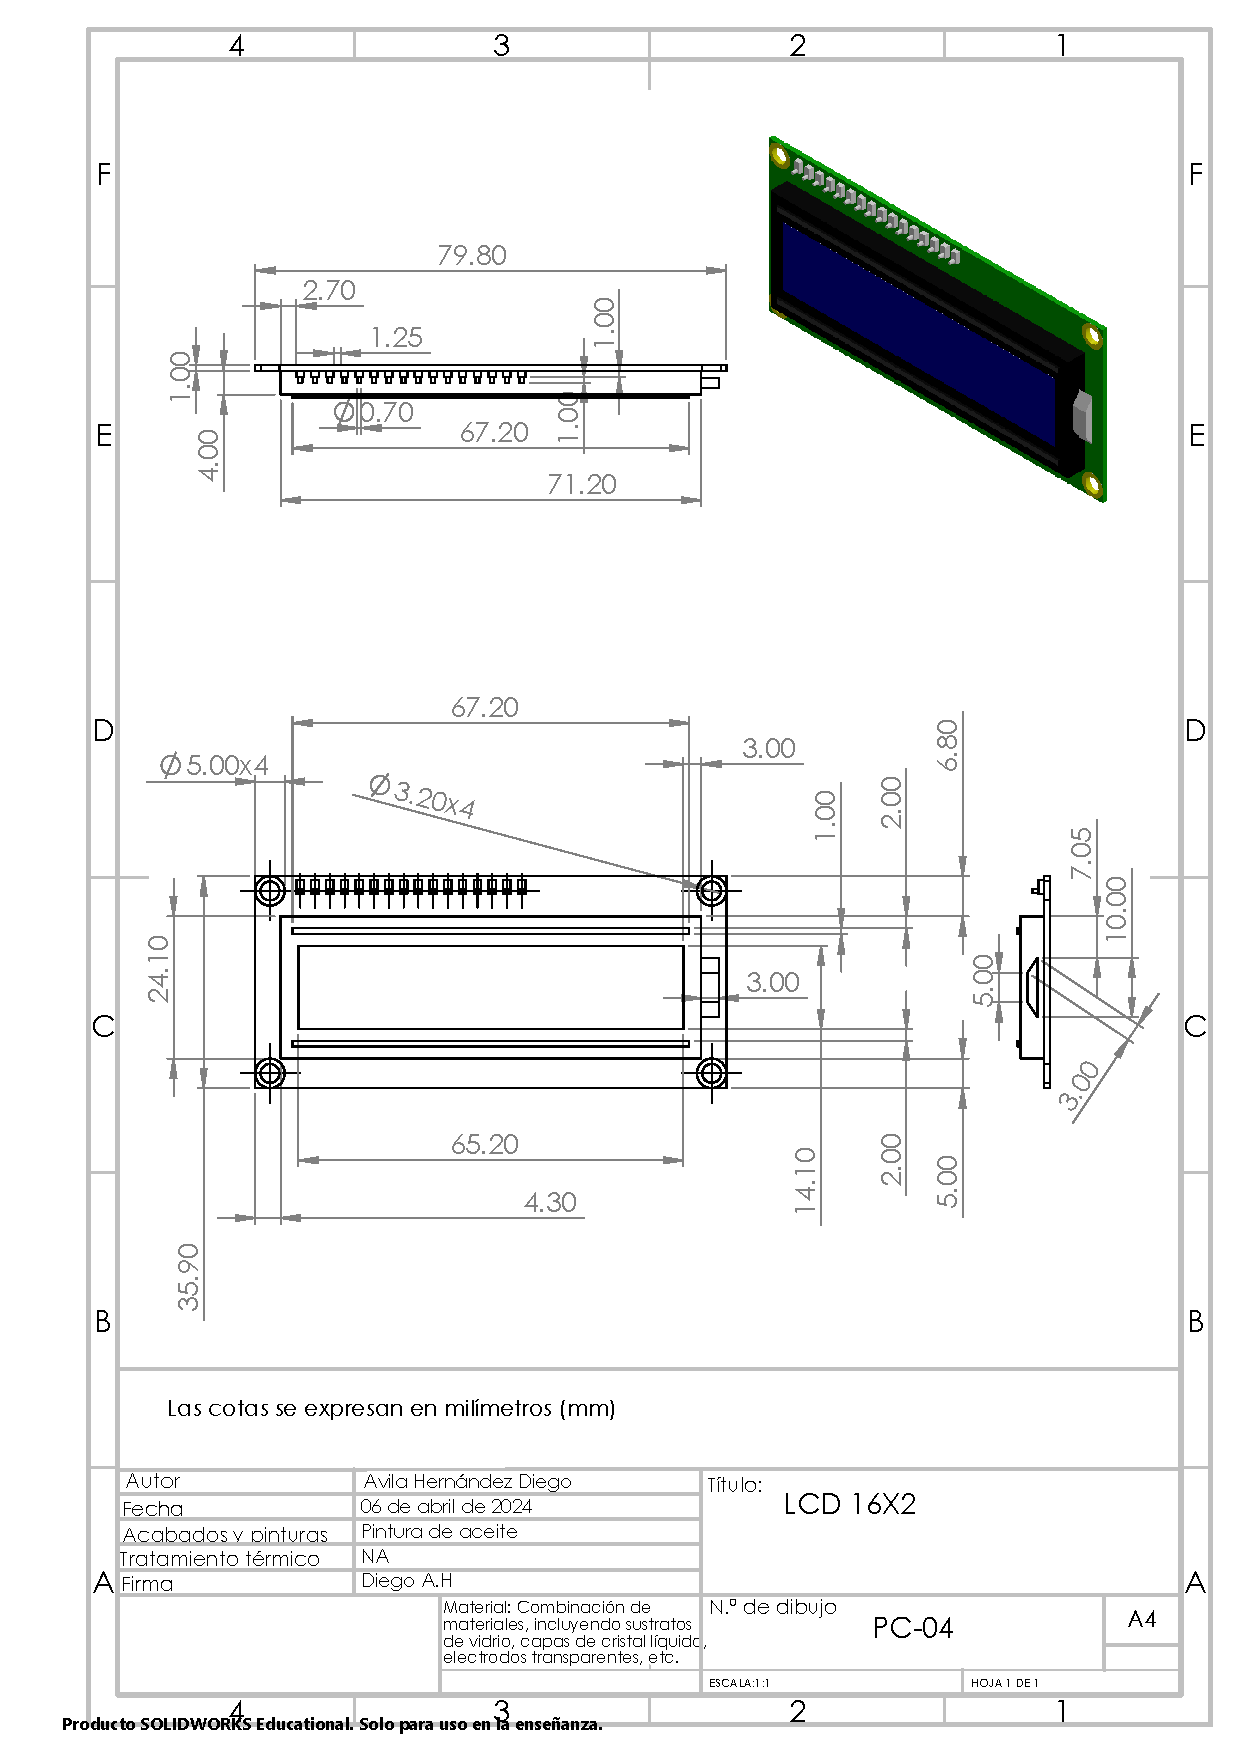
\includegraphics[scale=0.4]{3/Img/lcdDibujo.pdf}
        \caption{PC-04 LCD 16x2} 
        \label{fig:lcdDibujo}
    \end{figure}
    % 
    % 
    \begin{figure}[H]
        \centering
        \includegraphics[scale=0.4]{3/Img/móduloAdaptadorLcdDibujo.pdf}
        \caption{PC-05 Módulo adaptador LCD 1602} 
        \label{fig:móduloAdaptadorLcdDibujo}
    \end{figure}
    % 
    % 
    \begin{figure}[H]
        \centering
        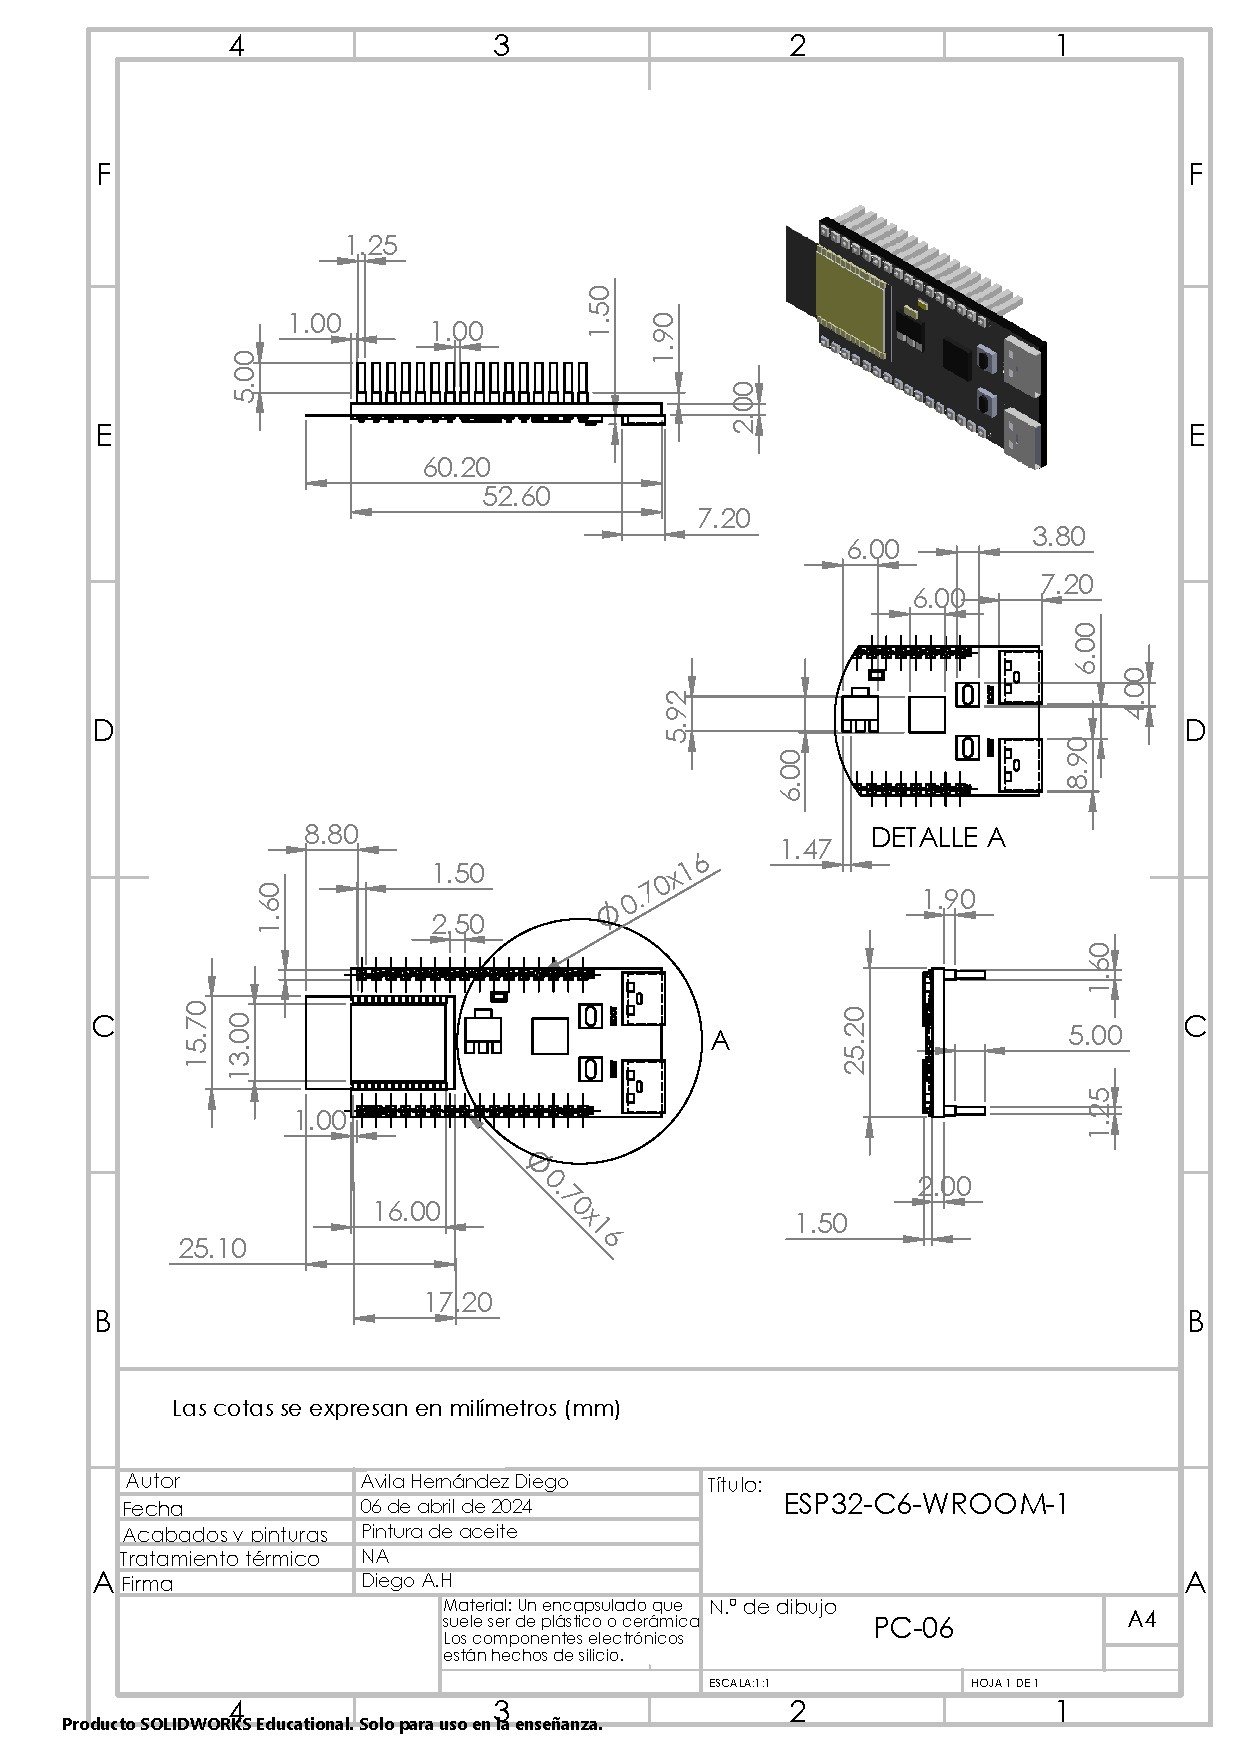
\includegraphics[scale=0.4]{3/Img/esp32Dibujo.pdf}
        \caption{PC-06 ESP32-C6-WROOM-1} 
        \label{fig:esp32Dibujo}
    \end{figure}
    % 
    % 
    \begin{figure}[H]
        \centering
        \includegraphics[scale=0.4]{3/Img/protoboardDibujo.pdf}
        \caption{PC-07 Protoboard} 
        \label{fig:protoboardDibujo}
    \end{figure}
    % 
    % 
    \begin{figure}[H]
        \centering
        \includegraphics[scale=0.4]{3/Img/resistenciaDibujo.pdf}
        \caption{PC-08 Resistencia 330 1/4 W} 
        \label{fig:resistenciaDibujo}
    \end{figure}
    % 
    % 
    \begin{figure}[H]
        \centering
        \includegraphics[scale=0.4]{3/Img/cableMHDibujo.pdf}
        \caption{PC-09 Cable MH 19cm} 
        \label{fig:cableMHDibujo}
    \end{figure}
    % 
    % 
    \begin{figure}[H]
        \centering
        \includegraphics[scale=0.4]{3/Img/cableMMDibujo.pdf}
        \caption{PC-10 Cable MM 19cm} 
        \label{fig:cableMMDibujo}
    \end{figure}
    % 
    % 
    \begin{figure}[H]
        \centering
        \includegraphics[scale=0.4]{3/Img/tapeteProfesionalOrganizadorDeTrabajoDibujo.pdf}
        \caption{PC-11 Tapete profesional organizador de trabajo} 
        \label{fig:tapeteProfesionalOrganizadorDeTrabajoDibujo}
    \end{figure}
    % 
    % 
    \subsubsection{Verificación}
    La planificación no salió como se había previsto, ya que durante el ensamblaje ocurrió un accidente que dañó la ESP-32, lo cual retrasó el trabajo porque solo teníamos una unidad. Para resolver este problema, decidimos comprar una nueva ESP-32. Sin embargo, nos dimos cuenta de que el envío tardaría al menos dos semanas en llegar. Ante esta situación, tomamos una decisión drástica: adquirir una ESP-32 de manera individual. Comparamos costos, calidad y tiempos de entrega. Finalmente, realizamos un pedido grande a través de una plataforma de compras en línea. La inversión final fue de 244 pesos ya que ese era su precio, sin embargo encargué una junto con mi compañera y nos ahorramos dinero. Por otra parte cabe mencionar que junto con mi compañera con quien estuve trabajando en el ensamble del circuito electrónico fuimos el primer equipo en armar el ensamble el día 25 de abril de 2024 , tardamos un poco en esa primer muestra por lo mismo de los nervios o por la incertidumbre de lo que podría pasar, afortunadamente todo salió bien y logramos concluir esa primer muestra. Para la segunda muestra que se realizó el 09 de mayo de 2024 nos fue mucho mejor, ya que nos sentimos más seguros y preparados, por lo cual logramos concluir dicha muestra. 
    \begin{enumerate}
    % 
    % 
    \item Véase las evidencias donde se comprueba que funcionó la primera muestra del armado del circuito electrónico:Figura\ref{fig:evidencia1}.\ref{fig:evidencia2}.\ref{fig:evidencia3}.\ref{fig:evidencia4}
    \begin{figure}[H]
        \centering
        \includegraphics[trim = {1mm 1mm 1mm 1mm},clip,scale=0.4]{3/Img/evidencia1.png}
        \caption{En esta imagen se observa cómo el operador conecta los cables al módulo adaptador LCD 1602} 
        \label{fig:evidencia1}
    \end{figure}
    % 
    % 
    \begin{figure}[H]
        \centering
        \includegraphics[trim = {1mm 1mm 1mm 1mm},clip,scale=0.4]{3/Img/evidencia2.png}
        \caption{En esta imagen se observa cómo el operador termina de conectar los cables en el módulo adaptador LCD 1602} 
        \label{fig:evidencia2}
    \end{figure}
    % 
    % 
    \begin{figure}[H]
        \centering
        \includegraphics[trim = {1mm 1mm 1mm 1mm},clip,scale=0.4]{3/Img/evidencia3.png}
        \caption{En esta imagen se observa cómo enciende el LCD 16x2 correctamente. Se alcanza a apreciar "Potenciómetro 1824"} 
        \label{fig:evidencia3}
    \end{figure}
    % 
    % 
    \begin{figure}[H]
        \centering
        \includegraphics[trim = {1mm 1mm 1mm 1mm},clip,scale=0.4]{3/Img/evidencia4.png}
        \caption{En esta imagen se observa cómo el operador mueve el potenciómetro para que se refleje el cambio en el LCD 16x2. Se alcanza a apreciar "Potenciómetro 1952"} 
        \label{fig:evidencia4}
    \end{figure}
    % 
    % 
        % \item Posición de las tablas y figuras: Coloque las figuras y las tablas en la parte superior e inferior de las columnas. Evite colocarlos en medio. Las figuras y las tablas grandes pueden abarcar ambas columnas. Los títulos de las figuras deben de estar debajo de las mismas; los títulos de las tablas deben aparecer encima de ellas. Insértese las figuras y los cuadros después de citarse en el texto. Utilice la abreviatura “Fig. 1”, incluso al principio de una oración. 
    \end{enumerate}
    % 
    % 
    \begin{enumerate}
    % 
    % 
    \item Véase las hojas de registro de las dos muestras realizadas \ref{fig:hojaDeRegistro1} \ref{fig:hojaDeRegistro2}
    % 
    %
    \begin{figure}[H]
        \centering
        \includegraphics[scale=0.4]{3/Img/hojaDeRegistro1.pdf}
        \caption{Hoja de registro 1} 
        \label{fig:hojaDeRegistro1}
    \end{figure}
    % 
    % 
    \begin{figure}[H]
        \centering
        \includegraphics[scale=0.4]{3/Img/hojaDeRegistro2.pdf}
        \caption{Hoja de registro 2} 
        \label{fig:hojaDeRegistro2}
    \end{figure}
    % 
    % 
    \end{enumerate}
    % 
    % 
    \subsubsection{Desarrollo del sistema de tiempos predeterminado}
    
    Al haber utilizado las tablas de Movimientos MTM-1, se desarrolló este diagrama bimanual. Véase la tabla donde se muestran los movimientos de la mano izquierda y la mano derecha. \ref{fig:diagramaBimanual1} 
    % 
    % 
    \begin{figure}[H]
        \centering
        \includegraphics[scale=0.4]{3/Img/diagramaBimanual1.pdf}
        \caption{Diagrama Bimanual} 
        \label{fig:diagramaBimanual1}
    \end{figure}
    % 
    % 
    \subsubsection{Desarrollo del muestreo del trabajo}
    
    Durante el desarrollo del proyecto, se identificó un problema debido a la falta de datos, específicamente la media y la varianza de nuestra población. Estos datos son esenciales en nuestro análisis para poder obtener los resultados deseados.
    Para lograr esto, se emplearon diversos métodos, incluyendo uno que utiliza probabilidades. Para calcular la media de la población, se aplicó la siguiente ecuación \ref{equ:media} y para  la desviación estándar utilizamos la ecuación \ref{equ:desviaciónestándar}. 
    % 
    % 
    \begin{equation}
                \label{equ:media}
               \mu = \dfrac{b+a}{2}
            \end{equation}
        
          \begin{equation}
                \label{equ:desviaciónestándar}
                \sigma = \sqrt{\dfrac{(b-a+1)^2-1}{12}}
            \end{equation}
    % 
    % 
    Para calcular el tiempo de ciclo, se diseñó un método de muestreo empleando un enfoque probabilístico. Se tomaron dos muestras en diferentes momentos, ya que estas son variables mutuamente excluyentes. Nuestro objetivo es encontrar una muestra que represente con precisión el valor real.
    Se creó una hoja de datos en Excel para calcular el tiempo de ciclo de cada elemento individualmente. Como nuestro trabajo se divide en 16 elementos, tenemos 16 tiempos de ciclo individuales, para calcular el tiempo de ciclo total inicial se sumaron los tiempos de ciclo individual. Por último para la
    obtención del tiempo estándar se calculó la desviación estándar de las dos muestras dado a que ésta tomara el lugar de los suplementos y holguras con ello el tiempo estándar se calculó con la ecuación \ref{equ:tiempoestándar}
    % 
    % 
    \begin{equation}
                \label{equ:tiempoestándar}
               TE= TC + \sigma
            \end{equation}
    % 
    % 
    Véanse las tablas donde se muestra el cálculo del tiempo de ciclo y así mismo el tiempo estándar en el ensamble del circuito electrónico \ref{fig:tiempoCicloYEstándarEnsamble} \ref{fig:tiempoCicloYEstándarEnsamble2}
    % 
    % 
    \begin{figure}[H]
        \centering
        \includegraphics[scale=0.4]{3/Img/tiempoCicloYEstándarEnsamble.pdf}
        \caption{Tiempo ciclo y tiempo estándar} 
        \label{fig:tiempoCicloYEstándarEnsamble}
    \end{figure}
    % 
    % 
    \begin{figure}[H]
        \centering
        \includegraphics[scale=0.4]{3/Img/tiempoCicloYEstándarEnsamble2.pdf}
        \caption{Continuación de la tabla anterior} 
        \label{fig:tiempoCicloYEstándarEnsamble2}
    \end{figure}
    % 
    % 
    Se utilizó un método probabilístico inicialmente. Sin embargo, debido a que esta sección se refiere al muestreo, se empleó una metodología diferente. Para ello, utilizamos las 2 muestras previamente seleccionadas, además de 8 muestras adicionales de 4 compañeros para realizar el muestreo de manera adecuada. En este método, también calculamos el promedio del tiempo de cada elemento para determinar el tiempo de ciclo individual. Luego, sumamos estos tiempos para obtener el tiempo de ciclo total del ensamblaje. Con los tiempos totales de cada muestra, también calculamos la varianza y la desviación estándar.
    Véanse las tablas donde se muestra el cálculo del tiempo de ciclo y así mismo el tiempo estándar en el ensamble del circuito electrónico al haber recolectado más lecturas. \ref{fig:tiempoCicloYEstándar10Lecturas} \ref{fig:tiempoCicloYEstándar10Lecturas2} \ref{fig:tiempoCicloYEstándar10Lecturas3} \ref{fig:tiempoCicloYEstándar10Lecturas4}
    % 
    % 
    \begin{figure}[H]
        \centering
        \includegraphics[scale=0.4]{3/Img/tiempoCicloYEstándar10Lecturas.pdf}
        \caption{Tiempo ciclo con las lecturas de mis compañeros parte 1} 
        \label{fig:tiempoCicloYEstándar10Lecturas}
    \end{figure}
    % 
    % 
    \begin{figure}[H]
        \centering
        \includegraphics[scale=0.4]{3/Img/tiempoCicloYEstándar10Lecturas2.pdf}
        \caption{Tiempo ciclo con las lecturas de mis compañeros parte 2} 
        \label{fig:tiempoCicloYEstándar10Lecturas2}
    \end{figure}
    % 
    % 
    \begin{figure}[H]
        \centering
        \includegraphics[scale=0.4]{3/Img/tiempoCicloYEstándar10Lecturas3.pdf}
        \caption{Tiempo ciclo y tiempo estándar con las lecturas de mis compañeros} 
        \label{fig:tiempoCicloYEstándar10Lecturas3}
    \end{figure}
    % 
    % 
    \begin{figure}[H]
        \centering
        \includegraphics[scale=0.4]{3/Img/tiempoCicloYEstándar10Lecturas4.pdf}
        \caption{Valor máximo, valor mínimo y rango} 
        \label{fig:tiempoCicloYEstándar10Lecturas4}
    \end{figure}
    % 
    % 
    \subsubsection{Corrección por balanceo de procesos}
    % 
    % 
    \subsubsection{Datos estándar continuos y discretos}
    % 
    %
    \subsection{Diseño de la forma más económica de realizar el trabajo}
    
    Después de ensamblar y analizar los tiempos estándar y los ciclos, realizamos un análisis para normalizar los materiales con el objetivo de encontrar la manera más económica de llevar a cabo el trabajo. para el análisis se cuenta con la siguiente tabla \ref{fig:tablaComparativaParaAnálisis}
    Con esta tabla, podemos comparar la diferencia de precios. A primera vista, puede parecer que el costo total de los materiales para el nuevo ensamblaje es mayor que el del ensamblaje antiguo. Sin embargo, nuestro objetivo es anticipar los posibles contratiempos que podrían surgir. Si no los prevemos con antelación, estos imprevistos pueden resultar más caros y generar mayores gastos debido a la urgencia de querer finalizar el ensamblaje. Esto nos llevaría a comprar materiales disponibles en lugar de los materiales necesarios.
    % 
    %
    \begin{figure}[H]
        \centering
        \includegraphics[scale=0.4]{3/Img/tablaComparativaParaAnálisis.pdf}
        \caption{Tabla comparativa para análisis de materiales} 
        \label{fig:tablaComparativaParaAnálisis}
    \end{figure}
    % 
    % 
    \subsection{Normalización de los métodos, materiales, herramientas e instalaciones}
    
    % 
    % 
    \subsection{Determinación del tiempo estándar para que una persona competente realice el trabajo con marcha normal}
    
    % 
    % 
    \section{Conclusiones}
    
    El propósito de este proyecto era crear un trabajo integrador a partir del montaje de un circuito, utilizando todos los temas vistos durante el semestre, como el estudio de movimientos y tiempos, así como muestras continuas o discretas. Además de aplicar los conocimientos adquiridos en Estudio del Trabajo II, también se buscaba complementar el proyecto con conocimientos de otras materias, como probabilidad y estadística, higiene y salud, y Estudio del Trabajo I.
    
    Nuestro objetivo principal era diseñar, mejorar e integrar sistemas productivos de bienes y servicios utilizando tecnologías para optimizarlos, con el fin de determinar el tiempo estándar para el ensamblaje del circuito.
    
    Sin embargo, el proyecto integrador no pudo completarse debido a diversas complicaciones surgidas a lo largo del semestre, como el retraso causado por la ESP32 y otros factores. A pesar de esto, el trabajo realizado no fue en vano, ya que adquirimos un conocimiento significativo sobre la normalización de procesos a nivel profesional. También aprendimos cómo los conocimientos de diferentes materias se complementan para ciertos trabajos, como fue el caso de este proyecto. Además, pudimos diseñar un manual de ensamblaje electrónico para capacitar a los operarios sin experiencia en este tipo de ensamblajes.
    
    Realizamos análisis de las pruebas de ensamblaje para identificar áreas de mejora y reducir costos, lo que haría más eficiente el proceso y facilitaría la tarea para los operarios. También nos familiarizamos con herramientas como Overleaf, GitHub y Visual Studio, que son ampliamente utilizadas en la industria y que adquirir experiencia con ellas durante el proyecto nos prepara para futuros trabajos.
    
    Al final, aunque no se pudo completar el proyecto integrador, logramos alcanzar la mayoría de nuestros objetivos y cubrir casi en su totalidad la hipótesis planteada. Este trabajo nos brindó una visión de los desafíos que enfrentaremos como ingenieros industriales en el futuro, y nos enseñó lecciones valiosas que serán de gran ayuda en nuestra carrera profesional.
    
    \section{Agradecimientos}
    
    Agradezco al profesor Luis Alberto Ángeles Hurtado por haber brindado su apoyo, conocimiento y experiencia para desarrollar este proyecto integrador, así como el seguimiento que nos dio y las retroalimentaciones que hizo, a mis compañeros que también me brindaron ayuda y en algunos casos resolvían mis dudas, también al Instituto Tecnológico de Querétaro que nos proporcionó información para enriquecer este proyecto integrador sobre el estudio de tiempos y movimientos en el ensamble de un circuito electrónico utilizando diferentes métodos para su optimización. 
    % 
    % 
    
    % \subsection{Prepara tu documento}
    
    % Antes de que comiences a utilizar esta plantilla, es recomendable que prepare la información que contendrá en un archivo aparte. 
    % Ten preparadas tus gráficas, así como también las tablas aparte, para que sea más fácil integrarlo. 
    % Se recomienda fuertemente el uso de \textbf{formato Enhanced Metafile (.emf) para imágenes y gráficas} de resolución óptima. 
    % Finalmente, completa y organiza el contenido antes de darle el formato de esta plantilla. 
    
    % \subsection{Acrónimos y Abreviaciones}
    
    % Los acrónimos y abreviaciones deberán ser definidos únicamente la primera vez que aparecen en el texto, esto para que el lector entienda lo que significan.
    
    % \subsection{Ecuaciones}
    
    % Las ecuaciones son una excepción a las especificaciones prescritas de esta plantilla. 
    % Deberá determinar si su ecuación debe escribirse o no utilizando la fuente Adobe Devangari. 
    % Para crear ecuaciones multinivel, puede ser necesario tratar la ecuación como un gráfico e insertarla en el texto después de aplicar el estilo de la platilla.
    % Las ecuaciones serán enumeradas de manera consecutiva, y el número de ecuación, entre paréntesis, se colocan al ras de la derecha, utilizando una tabulación derecha. 
    
    % \begin{equation}
        % \label{eq1}
        % x + y = z 
    % \end{equation}
    
    % Es importante asegurarse de que los símbolos de la ecuación sean definidos antes o inmediatamente después de la ecuación. Utilice “(1)”, en vez de “Eq. 1” al enumerar las ecuaciones, excepto al principio de una oración: “La ecuación (\ref{eq1}) es…”
    
    % \section{Resultados y discusión}
    
    Antes de comenzar a preparar tu artículo, es importante que lea primero la guía del autor, la cual incluye los temas o apartados que son necesarios para tener tu trabajo completo.
    Una vez completada la edición del texto, el documento está listo para el uso de esta plantilla. En este archivo recién creado, resalte todo el contenido e importe el archivo de texto preparado. Ahora esta listo para estilizar su documento.
    % En esta sección se deben presentar todo lo obtenido de la sección 2, incluidas deducciones o efectos del desarrollo. También se podrán incluir subsecciones numeradas de la siguiente forma:
    
    % \subsection{Autores y Afiliaciones}
    
    % Para distinguir las afiliaciones de los autores, utilice superíndices iniciando con el número 1, 2, etc., sucesivamente, esto dependerá de la cantidad de los departamentos a los que estén afiliados los autores. En caso de que todos los autores pertenezcan a una mismo departamento e institución, utilizar sólo el superíndice 1. 
    
    % \subsection{Identificar los encabezados}
    
    Se les recuerda a los autores que los encabezados deben de estar conforme los solicita la guía del autor. De ahí se puede adaptar el trabajo para que sea más fácil de entender para el lector.
    % Los encabezados organizan los temas sobre una base relacional y jerárquica. Por ejemplo, el título del documento es encabezado del texto principal porque todo el material posterior se relaciona y elabora sobre este tema. 
    
    % \subsection{Tablas y Figuras}
    
    % \section{Conclusiones}
    
    % Se describe aquí el alcance del trabajo, logros obtenidos y perspectivas para el futuro de este. Se sugiere colocar información cuantitativa obtenida.
    
    % \section{Agradecimientos}
    
    % Es importante darles su debido reconocimiento a los laboratorios, instituciones, organizaciones, entre otros que han sido participes para la culminación de este trabajo. También es importante mencionar, fondos, proyectos, becas, entre otros que se le han otorgado al o los autores para realizar el trabajo de investigación. Ejemplo: “Los autores agradecen al Concejo Nacional de Ciencia y Tecnología por los recursos otorgados…”
    
    % \section*{Referencias}
    
    % Para esta platilla, se solicita al autor enumerar las citas de manera consecutiva entre corchetes \cite{YLi2013}. 
    % La puntuación de la oración que sigues sería \cite{Mesaelides2011}. 
    % Refiérase simplemente al número de referencia, como en \cite{Morales2012}, no utilice “Ref. [3]” o “referencia [3]” excepto al principio de una oración: “La referencia [3] fue la primera…”
    % Enumere las notas al pie por separado en superíndices. Coloque la nota de pie de en la parte inferior de la columna en la que se citó. No coloque notas al pie en la lista de referencias. Utilice letras para las notas al pie de la tabla.
    % A menos de que haya tres autores o más; no utilice “et al.”. Los trabajos que no hayan sido publicados, incluso si han sido presentados para su publicación, deben ser citados como “inéditos”. Los trabajos que han sido aceptados para su publicación deben de citarse como “en prensa”. Poner en mayúscula sólo la primera palabra de un título, excepto los nombres propios y los símbolos de elemento. 
    % Otros ejemplos \cite{LAAngeles2021}, \cite{LAAngelesConni}. 
    % Véase el archivo adjunto \ref{anexo:pines}.
    
    % Ejemplo
    %  @Article{article,
    % 	author = "Author1 LastName1 and Author2 LastName2 and Author3 LastName3",
    % 	title = "Article Title",
    % 	volume = "30",
    % 	number = "30",
    % 	pages = "10127-10134",
    % 	year = "2013",
    % 	doi = "10.3389/fnins.2013.12345",
    % 	URL = "http://www.frontiersin.org/Journal/10.3389/fnins.2013.12345/abstract",
    % 	journal = "Frontiers in Neuroscience"
    % }
    
    % @book{book,
    %   author    = {Author Name}, 
    %   title     = {The title of the work},
    %   publisher = {The name of the publisher},
    %   address   = {The city},
    %   year      = 1993,
    % }
    
    % @incollection{chapter,
    %   author       = {Bauthor Surname}, 
    %   title        = {The title of the work},
    %   editor       = {Editor Name},
    %   booktitle    = {The title of the book},
    %   publisher    = {The name of the publisher},
    %   address      = {The city},
    %   year         = 2002,
    %   pages        = {201-213},
    % }
    
    % @InProceedings{conference,
    %   author = {Cauthor Name and Dauthor Surname and Fauthor LastName},
    %   title = {The title of the work},
    %   booktitle = {The title of the conference proceedings},
    %   year = 1996,
    %   publisher = {The name of the publisher},
    %   editor = {Editor Name1 and Editor Name2},
    %   pages = {41-50},
    % }
    
    % @book{cho,
    %   author       = {Gauthor Name1}, 
    %   title        = {The title of the work},
    %   publisher = {Country code and patent number},
    %   address      = {Patent Country},
    %   year = 2013
    % }
    
    % @book{patent,
    %   author    = {Hauthor Surname1}, 
    %   title     = {The title of the work},
    %   publisher = {Patent number},
    %   address   = {Patent country},
    %   year      = 2010,
    % }
    
    % % please use misc for datasets
    % @misc{dataset, 
    % 	author = "Author1 LastName1 and Author2 LastName2 and Author3 LastName3",
    % 	title = "Data Title",
    % 	year = "2011",
    % 	doi = "10.000/55555",
    % 	URL = "http://www.frontiersin.org/",
    % }
    % 
    % 
    \bibliographystyle{ieeetr}
    \bibliography{3/referencias}
    %
    %
    \newpage
    %%%%%%%%%%%%%%%%%%%%%%%%%%%%%%%%%%
    \appendix
    %%%%%%%%%%%%%%%%%%%%%%%%%%%%%%%%%%
    % 
    % 
    \centering{\section[\appendixautorefname{}]{}}\label{anexo:hojaDeRegistro}
    \includepdf[pages=-]{3/Img/hojaDeRegistro.pdf}
    %%%%%%%%%%%%%%%%%%%%%%%%%%%%%%%%%%%%%%%%
    % 
    % 
    %%%%%%%%%%%%%%%%%%%%%%%%%%%%%%%%%%
    \appendix
    %%%%%%%%%%%%%%%%%%%%%%%%%%%%%%%%%%
    % 
    % 
    \centering{\section[\appendixautorefname{}]{}}\label{anexo:ensambleDeCircuitoElectrónico1}
    \includepdf[pages=-]{3/Img/ensambleDeCircuitoElectrónico1.pdf}
    %%%%%%%%%%%%%%%%%%%%%%%%%%%%%%%%%%%%%%%%